\chapter{Performance}
\label{ch:performance}

% =============================================================================================== %
% \textbf{This chapter is now complete - but wasn't in the first three chapter draft submission!} %
% =============================================================================================== %

As enumerated in the objectives summary section of the introduction, one of the three requirements for Rust's suitability as a language for High-Performance Computing is having a comparable performance to C++, one of the most commonly used languages in current usage.

This chapter provides an empirical assessment of the performance of the Rust translation of the HPCCG mini-app. As discussed in the background section \ref{ssec:hpccg} introducing HPCCG, this is representative of High-Performance Computing workloads as a result of the design goals of Mantevo Suite to facilitate hardware-software co-design. We leverage this property to instead assess the Rust language's suitability for such workloads by comparing the performance of the Rust translation to the original C++ implementation.

This performance profiling will begin with the use of performance profiling tools to identify hot-spots and hardware under-utilisation in source code. These tools also allow direct comparisons of compiled assembly, yielding a clear picture of ways in which the Rust language differs from C++. Then, the HPC MultiBench tool will be used to run and analyse direct measurements of the Rust and C++ codebases. This allows the characterisation and comparison of performance for strong and weak scaling, and parallelism approaches.

\section{Profiling tools}
\label{sec:profiling-tools}

Software profilers are a category of tools which are used to measure properties of running programs. This is in contrast to static analysis tools, which use only the source code itself. Profilers are most often used to characterise the performance and memory usage of programs, and through instrumentation can identify ``hotspots'' -- code sections in the program which account for a disproportionate amount of the metric, such as overall runtime. This makes profilers useful for guiding optimisations, as engineering effort can be targeted at the portion of program which impacts performance most greatly.

Performance profilers can also be used to compare implementations of the same software in different languages. Comparing the  profiles of the programs on the same problem size can elucidate where one language loses performance over another, and give insights into key factors such as vectorisation and memory bandwidth utilisation.

% We choose to use a variety of performance profilers, because some profilers provide many more metrics and analysis options, but typically at the expense of the simple and ergonomic user interface. As a result of this, we used \texttt{perf} for the majority of profiling tasks, as they provide a convenient command line interface for instrumentation statistical sampling. We also used the Intel\textsuperscript{\textregistered}\ oneAPI\texttrademark\ suite of tools, including Intel\textsuperscript{\textregistered}\ vTune\texttrademark\ and Intel\textsuperscript{\textregistered}\ Advisor\texttrademark, as these provide a vast array of capabilities such as roofline analysis, but with a complex graphical-only interface.


\subsection{The \texttt{perf} profiler}
\label{ssec:perf-profiler}

\texttt{perf} is a performance analysis tool which has been part of the Linux kernel since the 2.6.31 release in 2009 \cite{PerfcountersAddedMainline}. It uses a ``git-like'' subcommand based command line interface  \cite{de2010new}, which allows it to perform many functionalities. The \texttt{record} subcommand uses a single kernel syscall to instrument statistical sampling or program performance, and the \texttt{report} subcommand presents an analysis of this recorded data.

The \texttt{perf} profiler was used throughout the translation process to identify hotspots in the code. The benefit of this process was two-fold. Firstly, it allowed manual performance-guided optimisation, allowing prioritisation of engineering effort to ensure the Rust implementation was a fair representation of the full extent of the language's capabilities when comparing it to C++. Secondly, the hotspots identified provided a strong insight into the parts of Rust programs that fall short of C++, which informs the assessment of the suitability of Rust for High-Performance computing applications.

% TODO: Assess overlap here with translation section
The Rust programming language places a strong focus on the prevention of undefined behaviour, including enforcing memory and thread safety. The key insight of the language was that many of these guarantees against undefined behaviour can be made at compile time, through the ownership model enforced by the borrow checker. However, there is not enough information at compile time to fully guarantee these characteristics. For example, creating a vector of a length provided by user input at run time is a common operation within many programs. However, if the programmer accesses this vector by a fixed index in the source code, the compiler cannot guarantee the indexing operation is within the bounds of this vector, since its size is not known until runtime. To avoid undefined behaviour, Rust checks the bounds of every indexing operations to guarantee that the index is not out of range, but this incurs a performance cost -- roughly doubling the time taken for vector indexing. To avoid this check in performance critical applications when the bounds are already guaranteed, Rust provides the \mintinline{rust}{get_unchecked} function, which does not perform the bound check. This performance cost can be seen through comparing \texttt{perf} reports when using the default bounds checked indexing in Figure \ref{fig:perf-checked}, against unchecked indexing in Figure \ref{fig:perf-unchecked}.

\begin{figure}[H]
    \centering
    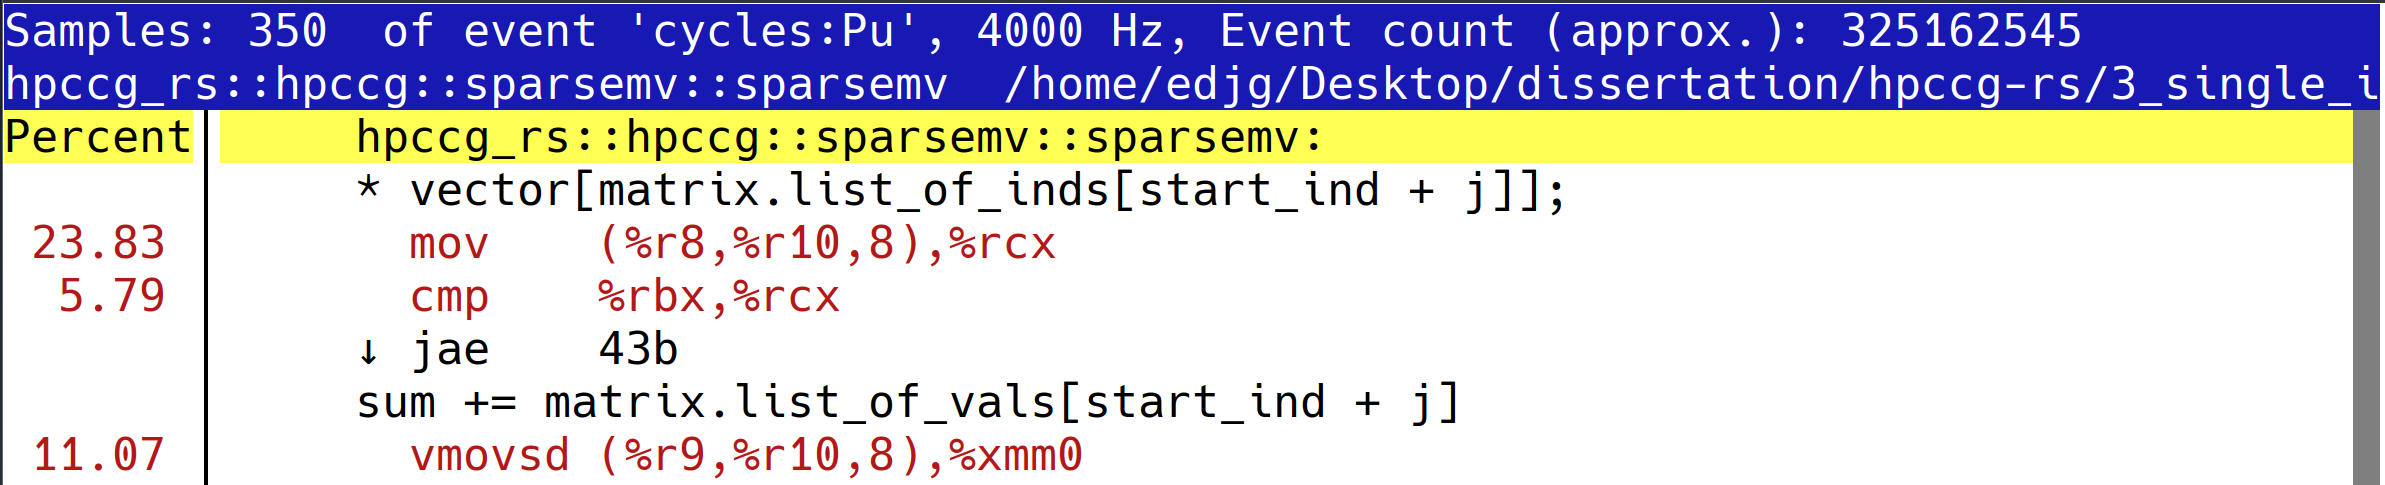
\includegraphics[width=0.95\textwidth]{images/5_performance/perf/perf_checked_op.png}
    \caption{A screenshot of the \text{perf} report of a Rust translation of HPCCG using the default checked indexing.}
    \label{fig:perf-checked}
\end{figure}

\begin{figure}[H]
    \centering
    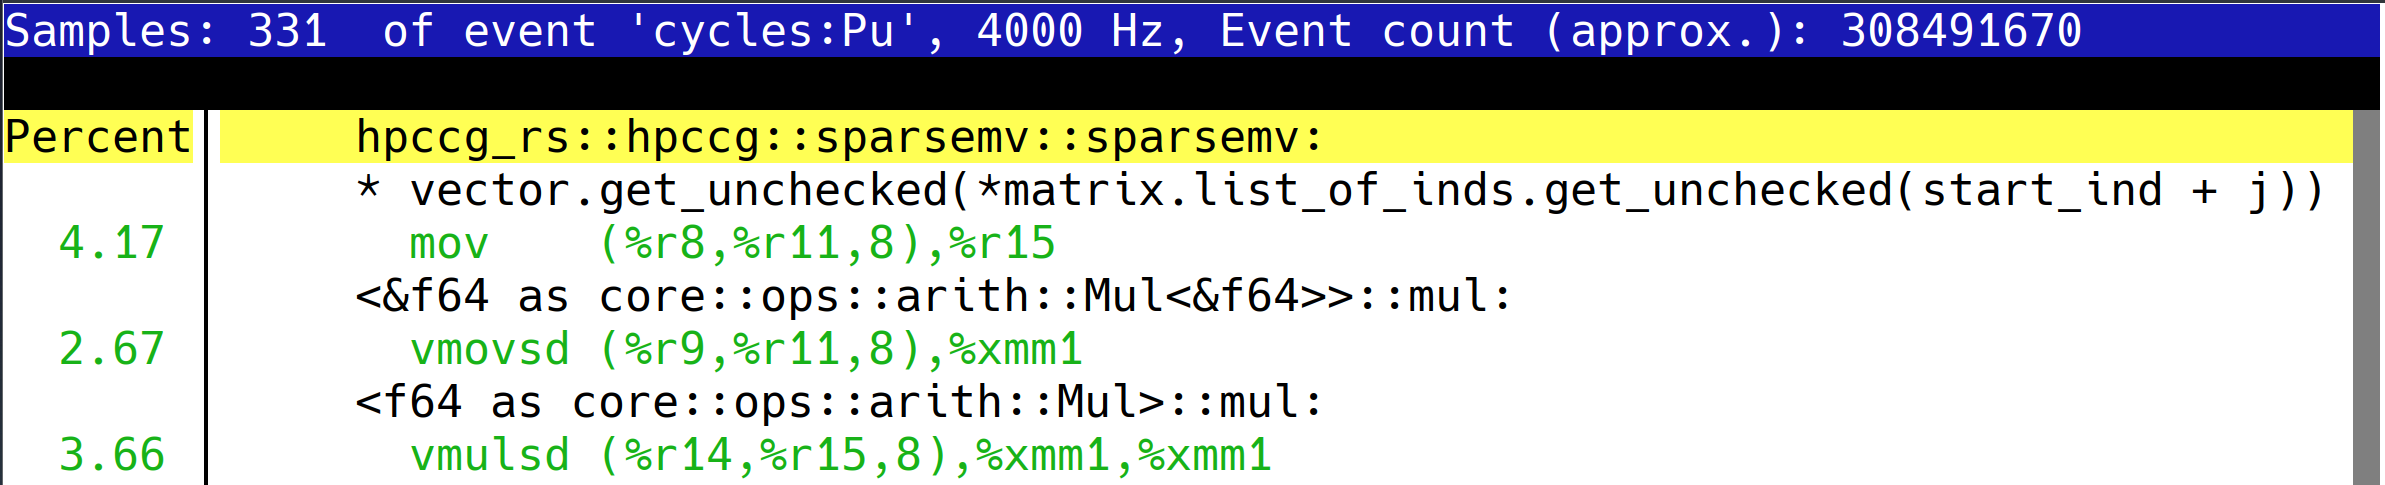
\includegraphics[width=0.95\textwidth]{images/5_performance/perf/perf_unchecked_op.png}
    \caption{A screenshot of the \text{perf} report of a Rust translation of HPCCG using the unchecked indexing.}
    \label{fig:perf-unchecked}
\end{figure}

From these figures, we can see that the bounds checking operation dominate the total runtime of the program, with $23.83 + 5.79 = 29.62$ percent of the runtime being taken up by the \mintinline{rust}{vector[matrix.list_of_inds[start_ind + j]]} operation in the bounds checked version, but only $4.17 + 2.67 + 3.66 = 10.5$ percent in the version without bounds checking. The empirical result of a $2.82\times$ speed-up for array indexing, a very common operation in High-Performance computing workloads, demonstrates the utmost importance of understanding and leveraging the full extent of the Rust language to be able to write performant software.

\subsection{The Intel\textsuperscript{\textregistered}\ oneAPI\texttrademark\ suite}
\label{ssec:intel-advisor-profiler}
% Intel vTune Advisor
% Roofline model

\subsubsection{Roofline models}
\label{sssec:roofline-models}

In their seminal paper ``Roofline: an insightful visual performance model for multicore architectures'', Williams, Waterman and Patterson introduce the roofline model as a technique for simply characterising performance in complex systems \cite{williamsRooflineInsightfulVisual2009}. The model combines three metrics: Computational performance, memory bandwidth, operational intensity.

Computer hardware can be modelled as three components: execution units, data sources, and the interconnection between them. Computational performance measures how fast these execution units can process data in FLOP/s, and memory bandwidth measures the rate at which data can be transmitted across the interconnection in Bytes/s. As computational performance, memory bandwidth quantify hardware performance, operational intensity quantifies software performance. It refers to the average amount of data required per operation in a program, in FLOPS/byte. Rooflines are then drawn, as shown in Figure \ref{fig:ert-roofline}, on a log-log axis, with the ``loft'' being a 45 degree line sloping up, and the ``ceiling'' a horizontal line.
% TODO: Improve this explanation

\begin{figure}[H]
    \centering
    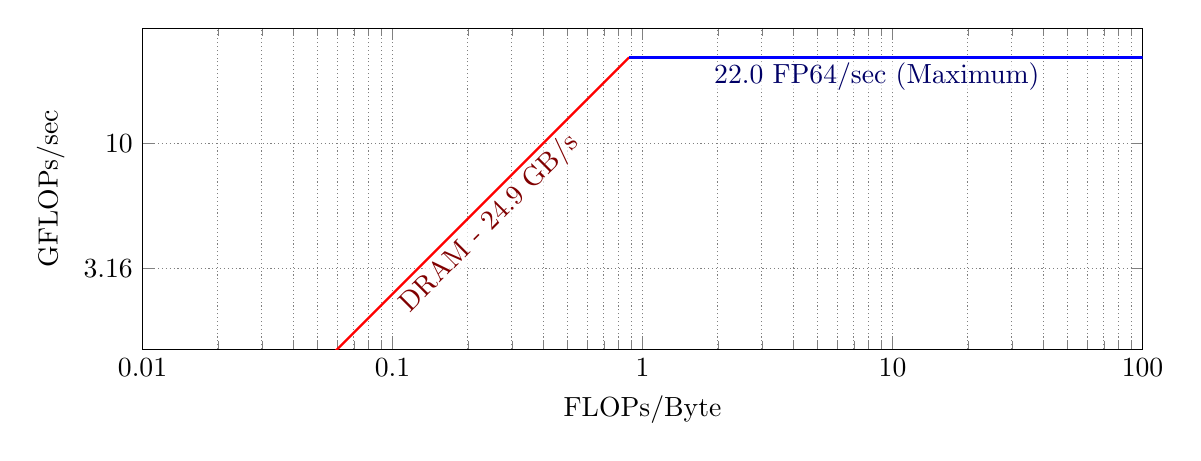
\begin{tikzpicture}
  \pgfplotsset {
    scale only axis,
    axis equal image,
    width=5in,
    /pgf/number format/1000 sep={},
    /tikz/maxline/.style={blue, thick, no marks},
    /tikz/memline/.style={red, thick, no marks},
    /tikz/maxlabel/.style={blue!40!black, right, fill=white, fill opacity=0.7, text opacity=1.0, rounded corners=2pt, inner sep=0.5pt},
    /tikz/memlabel/.style={red!50!black, rotate=45, right, fill=white, fill opacity=0.7, text opacity=1.0, rounded corners=2pt, inner sep=0.5pt}
  }

  \def\Xmin{1.000000e-02}
  \def\Xmax{1.000000e+02}

  \begin{loglogaxis}[
    grid=both,
    grid style={black!50, densely dotted},
    xlabel= FLOPs/Byte,
    ylabel= GFLOPs/sec,
    xmin=\Xmin,
    xmax=\Xmax,
    ymin=1.500000e+00,
    ymax= ,
    log ticks with fixed point
    ]

    \node[maxlabel] at (axis cs: 1.9000000e+00,1.8448000e+01) {22.0 FP64/sec (Maximum)};
    \node[memlabel] at (axis cs: 1.1036459e-01,2.1571047e+00) {DRAM - 24.9 GB/s};
    \addplot[memline, domain=(\Xmin:8.8336673e-01)] {2.4950000e+01*x};
    \addplot[maxline, domain=(8.8336673e-01:\Xmax)] {2.2040000e+01};

  \end{loglogaxis}
\end{tikzpicture}
    \vspace*{-0.5cm}
    \caption{A roofline graph, modified from the output of the Empirical Roofline Tool \cite{EmpiricalRooflineTool}.}
    \label{fig:ert-roofline}
\end{figure}

The paper summarises the roofline model as ``set[ing] an upper bound on performance of a kernel depending on the kernel’s operational intensity. If we think of operational intensity as a column that hits the roof, either it hits the flat part of the roof, meaning performance is compute-bound, or performance is ultimately memory-bound'' \cite{williamsRooflineInsightfulVisual2009}. This allows the easy identification of where optimisations for the kernel might be possible, based on its position with respect to the roofline. Finally, the paper explains how SIMD instructions can be represented as additional ceilings, as the peak attainable computational performance of such vectorised instructions is necessarily higher.

% Later, Ilic, Pratas and Sousa proposed a modification to the roofline model to include information about cache bandwidths in their paper ``Cache-aware Roofline model: Upgrading the loft'' \cite{ilic_cache-aware_2014}. This adds multiple ``lofts'', as the memory bandwidth of caches are higher that of main memory. In addition to this, SIMD instructions can result in additional ceilings, as the peak attainable computational performance of vectorised instructions is necessarily higher.

Roofline models are a powerful technique to simply characterise the bottlenecks in software. As such, tools such as the Intel\textsuperscript{\textregistered}\ Advisor can be used to generate them.

\subsubsection{Generating rooflines with Intel\textsuperscript{\textregistered}\ Advisor}
\label{sssec:roofline-generation-intel-advisor}

The Intel\textsuperscript{\textregistered}\ Advisor tool is part of the Intel\textsuperscript{\textregistered}\ oneAPI\texttrademark\ suite. Intel describes it as ``a design and analysis tool for developing performant code'' \cite{DesignCodeParallelism}, and one of the functionalities it provides is generating roofline plots. This is commonly done using its graphical user interface, but it is possible to also generate plots as minified HTML files from the command line. Listing \ref{listing:roofline-generation} shows the sequence of commands required to generate the roofline plots for an executable. 

\begin{code}
    %TC:ignore
    \begin{minted}{bash}
        advisor -collect roofline -project-dir ./ -- ./test_HPCCG
        advisor --report=roofline --project-dir=./ --report-output=./roofline.html
    \end{minted}
    %TC:endignore
    \caption{The commands required generate roofline models from the command line.}
    \label{listing:roofline-generation}
\end{code}

Using these plots, we can characterise whether the computational kernels are memory or compute bound in each language, which gives an insight into how their performance can be improved.

Roofline plots can be applied to multithreaded and distributed workloads, however assuming a uniform processor architecture, the degree of parallelism does not significantly impact whether the kernels are computer or memory bound. As such, roofline plots for multithreaded and distributed workloads are not included here, as they are not relevant and often less clear. Figure \ref{fig:cpp-roofline} shows the roofline plot for the C++ implementation of HPCCG, and Figure \ref{fig:rust-roofline} for plot for the Rust translation.

\begin{figure}[H]
    \centering
    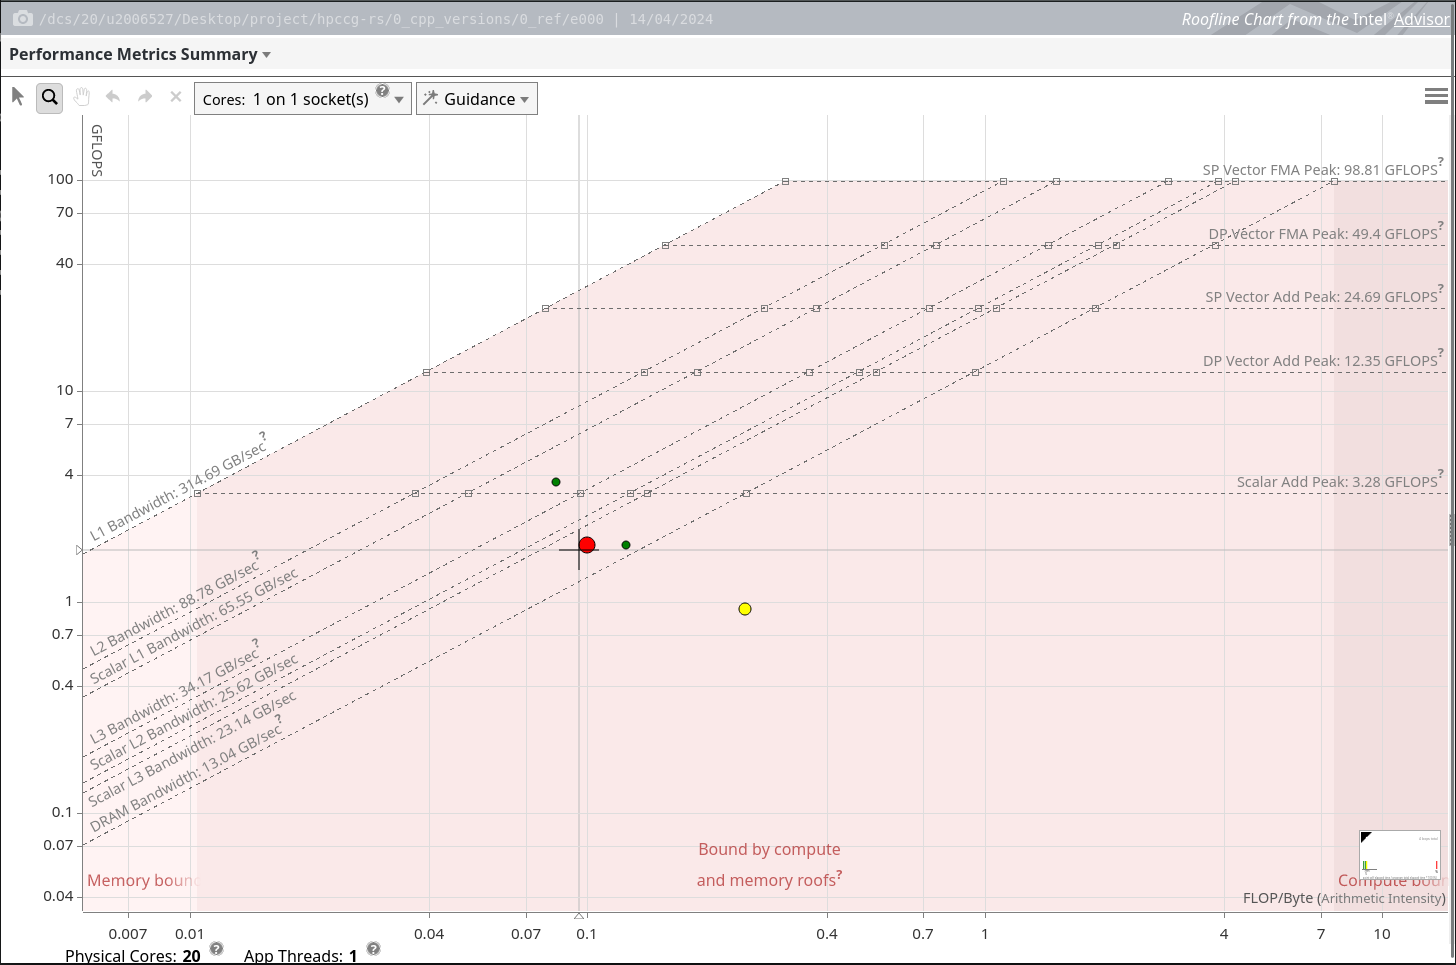
\includegraphics[width=0.85\textwidth]{images/5_performance/rooflines/cpp_roofline.png}
    \caption{A roofline diagram generated by Intel\textsuperscript{\textregistered}\ Advisor\ showing the performance of the C++ implementation of HPCCG.}
    \label{fig:cpp-roofline}
\end{figure}

\begin{figure}[H]
    \centering
    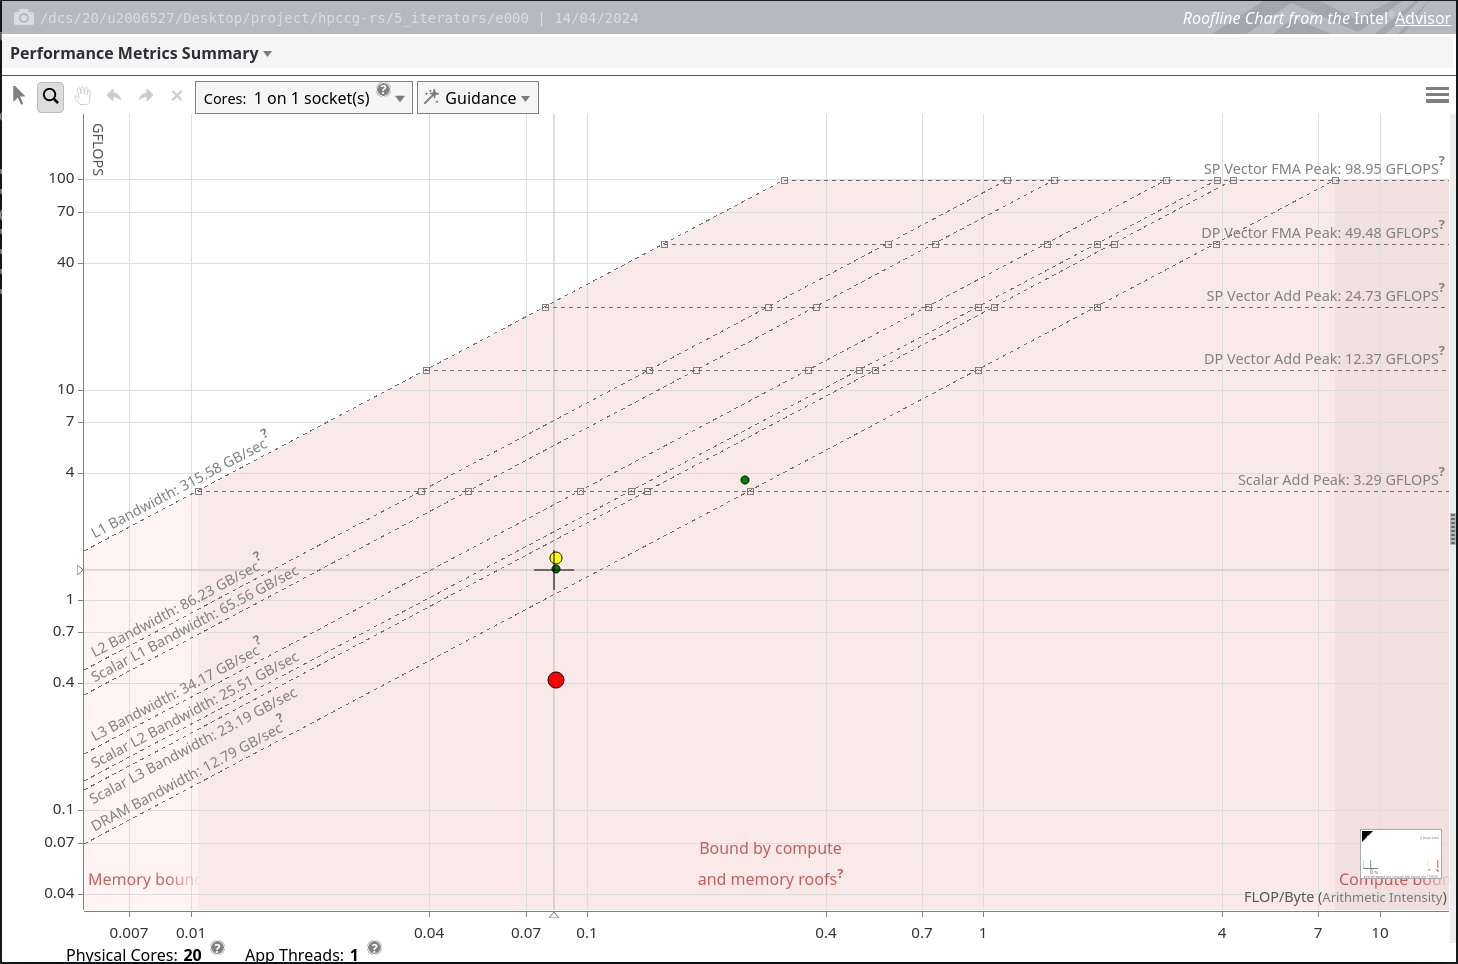
\includegraphics[width=0.85\textwidth]{images/5_performance/rooflines/rust_roofline.png}
    \caption{A roofline diagram generated by Intel\textsuperscript{\textregistered}\ Advisor\ showing the performance of the Rust translation of HPCCG.}
    \label{fig:rust-roofline}
\end{figure}

From these plots, we can see that both the C++ and Rust implementations appear to be mostly memory bound, with the DRAM bandwidth limiting the performance of the functions. Since these rooflines were generated on very small meshes of size $25 \times 25 \times 25$, to avoid overloading Intel\textsuperscript{\textregistered}\ Advisor with data samples, we can see that some of the kernels for both implementations are within the cache section of the plot. This is because the mesh data is small enough to be fully included in cache memory. We can also see that the \texttt{waxpby}, shown by the upper green dot in Figure \ref{fig:cpp-roofline}, in the C++ is amenable to vectorisation, and as such is able to exceed the scalar compute roofline. Finally, the locations of the kernels across the plots differ fairly significantly, indicating the different software loads have different performance characteristics across the two languages.

Overall, C++ has both a higher arithmetic intensity and rate of floating point operations, which indicates it is able to make better use of the compute hardware it runs on. As a result of this, we expect direct measurements of the C++ program to have slightly higher performance.

In addition to using the Intel\textsuperscript{\textregistered}\ Advisor, HPC MultiBench supports plotting rooflines for performance characterisation at a glance as part of larger test plans. It parses JSON data generated by the Empirical Roofline Tool \cite{EmpiricalRooflineTool} to generate the ceilings, and the Likwid toolkit \cite{RRZEHPCLikwid2024} to calculate operational intensity and performance. An example of this capability is shown in Figure \ref{fig:hpc-multibench-roofline}, which is able to render multiple different executables on the same plot for comparison.

\begin{figure}[H]
    \centering
    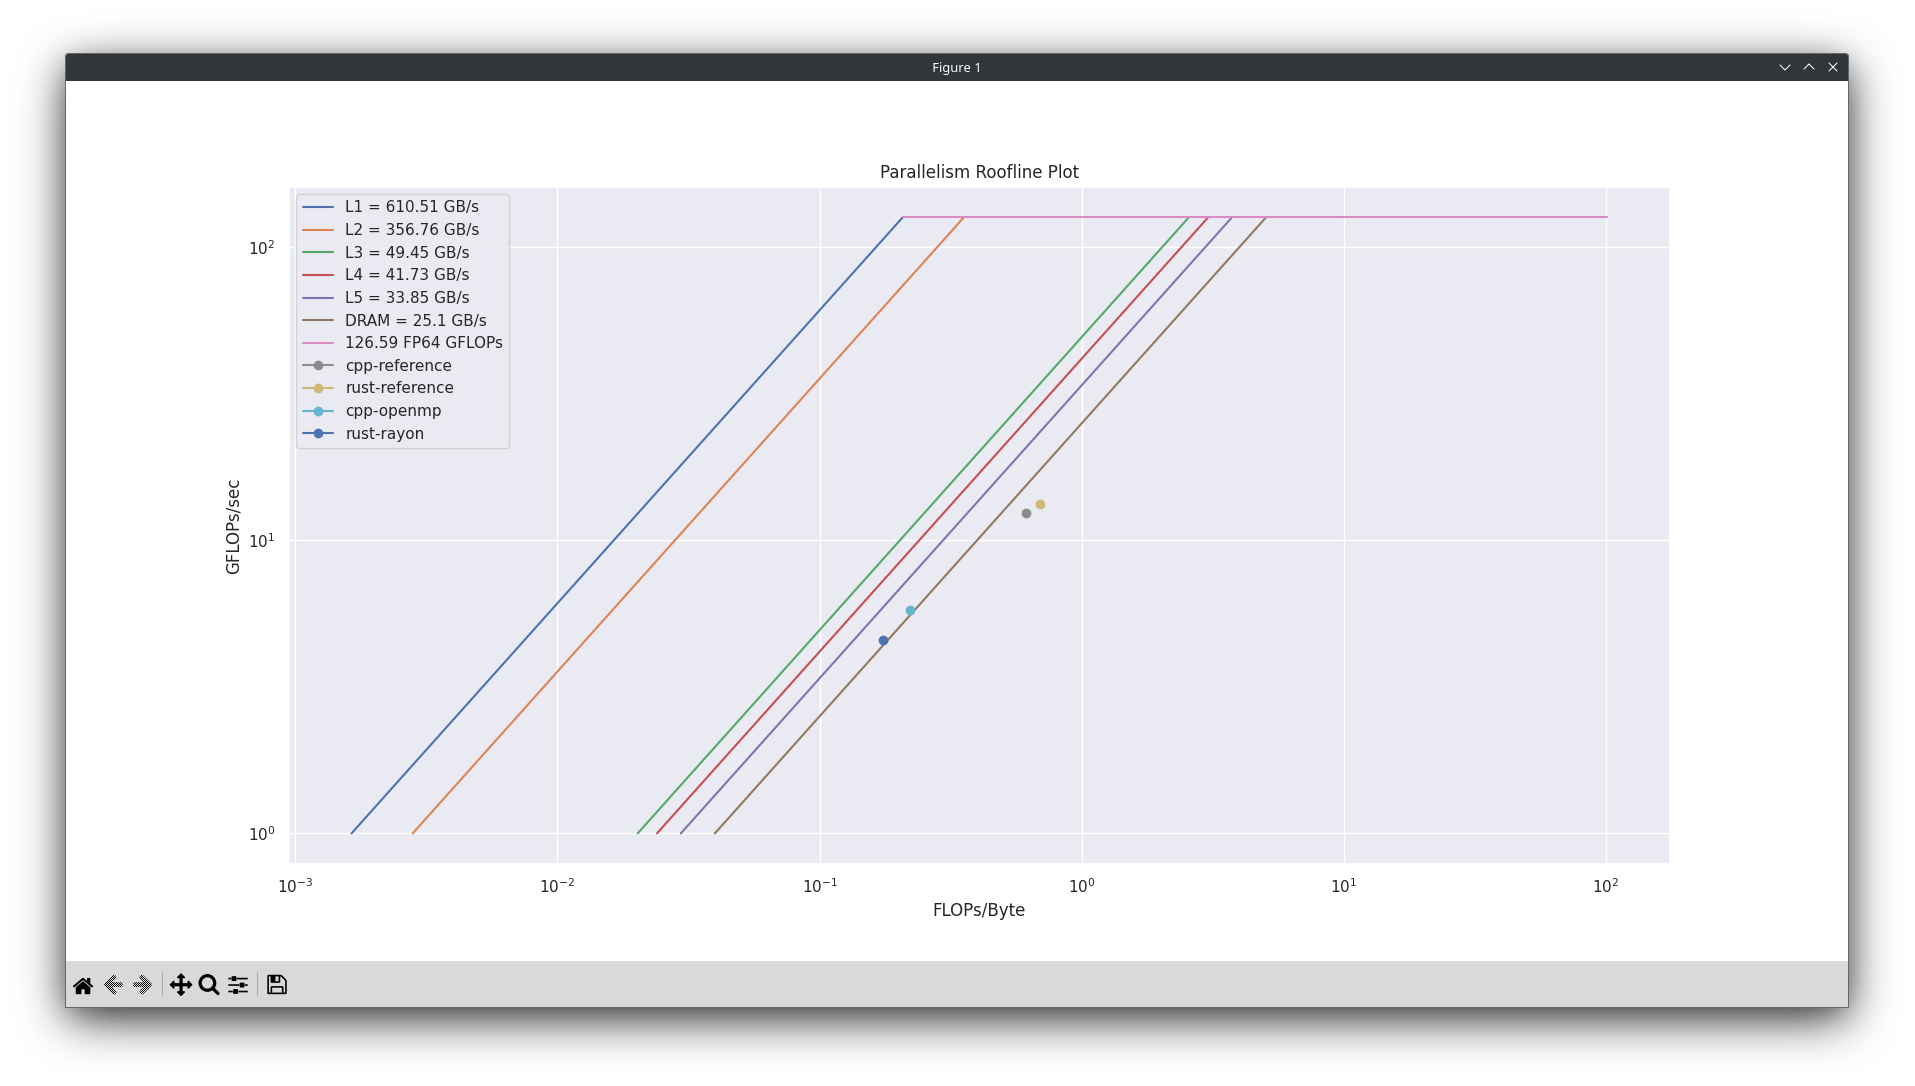
\includegraphics[width=\textwidth]{images/4_tooling/interactive_screenshots/hpc-multibench-roofline-matplotlib.png}
    \caption{A roofline diagram generated by HPC MultiBench comparing the performance characteristics of the C++ and Rust versions of HPCCG.}
    \label{fig:hpc-multibench-roofline}
\end{figure}

This figure confirms the statement that the mini-app is memory bound, and shows that employing multi-threading techniques allows implementations to better leverage the hardware they are run on.

Performance profilers provide a very powerful tool for identifying and optimising away hotspots in running programs. However, profilers are typically best suited for measuring many performance metrics in a fixed configuration, such as with a set number of processor threads or MPI ranks. To assess Rust's suitability for High-Performance Computing, we only needed a few metrics such as runtime and FLOPs, but wanted to measure how these varied across a wide range of metrics, with statistical confidence. As a result of this, we switched to a direct measurement approach driven by the HPC MultiBench tool, which was designed for this purpose.

\section{Direct measurement}
\label{sec:direct-measurement}

For Rust to be a suitable language for High-Performance Computing workloads, it must have a comparable performance across both a range of parallelism approaches, from serial execution to multi-threading and message passing across a compute cluster, and for large data volumes. To assess this, measured the execution time of the original C++ and translated Rust implementations of HPCCG across a variety of problem sizes, and a variety of thread counts and MPI sizes.

\subsection{Experimental methodology}
\label{ssec:experimental-methodology}

% TODO: Add this note
% In the intro to the book Performance Tuning of Scientific Applications, David Bailey suggests nine guidelines for presenting performance results without misleading the reader. Paraphrasing only slightly, these are: 

The experiments are fully defined by the YAML configuration files for the HPC MultiBench tool, providing extremely strong reproducibility characteristics. The salient features this provides include driving the programs across a range of inputs and configurations, along with supporting re-runs to give statistical confidence in the results.

For all experiments in this results section, the programs are run five times. The slowest run is then always discarded as an outlier, due to the possibility of machine noise or network instability for MPI workloads.

The original HPCCG implementation provides a number of different timers which measure the computational kernels. These include clock ticks, resource usage, wall time, and MPI timing intrinsics. By default, resource usage is used for serial and threaded compilations, and MPI timing intrinsics when MPI is used. However, the resource usage timer records the sum of the times for each thread. As a result of this, the \texttt{-DWALL} compiler flag was set to use the wall time. This allows representative comparisons to be made, as otherwise Rust may record faster times for short runs as a result of Rayon's work-stealing threading model. Finally, the UNIX \texttt{time} utility was also used to measure the total runtime including matrix setup, rather than just computational kernel runtimes.

On Kudu, 60GB of RAM was used, and on Avon 40GB was used, the maximum available memory for their respective compute nodes. During development, smaller RAM sizes were used, resulting in significantly degraded performance as a result of the mesh sizes exceeding allocated RAM, resulting in memory thrashing \cite{pattersonHennessyComputerOrganisationArchitecture}. To mitigate this, these very large RAM sizes were used, which guarantees thrashing does not occur since the mesh size does not exceed the amount of memory used, even for the largest mesh sizes of $400 \times 400 \times 400$.


\subsubsection{Reproducibility}
\label{sssec:parallelism-approaches-reproducibility}

% TODO: Check line wrapping here
The raw data files and test plan YAML files for the results are available in the base and \texttt{\_test\_plan} directories of the \mintinline[breaklines,breakafter=-]{text}{hpccg-rs-kudu-results} and \mintinline[breaklines,breakafter=-]{text}{hpccg-rs-avon-results} repositories for the two compute systems respectively. Listing \ref{listing:serial-data-interactive} shows the command to launch the interactive user interface for the Kudu and Avon test plans respectively. When run locally, this allows the aggregation and analysis of the generated results to be viewed. If run on the appropriate batch computer system, the test benches can be re-run with the ``Run Test Plan'' button.

\begin{code}
    %TC:ignore
    \begin{minted}{bash}
poetry run hpc_multibench \
    -y generated_results/hpccg-rs-kudu-results/ _test_plans/parallelism.yaml \
    interactive
    \end{minted}
    %TC:endignore
    \caption{The commands required to interactively view and re-run the performance experiments for the parallelism approaches test benches on the Kudu batch compute system.}
    \label{listing:serial-data-interactive}
\end{code}

This yet again shows the power of the HPC MultiBench tool beyond the example use case shown in section \ref{ssec:hpc-multibench-replication-study}, as the experimental results presented in the previous section can easily be reviewed and even re-run, using a single command.


\subsubsection{System specifications}
\label{sssec:system-specifications}

During the course of experimentation, three different compute resources were used: Athena, the author's personal laptop; Kudu, the DCS batch compute system; and Avon, the Warwick SCRTP High-Performance Computing resource. Athena was used for the translation effort and initial testing, but not for any experimental results. However, since tests during the development process informed design decisions, its system specifications are relevant. Kudu was used for the majority of testing and the project presentation demo, as it is easy to access and has short queue times. Avon was used for later tests to confirm results, and for very large tests which exceeded Kudu's nodal capacity.

To best allow for reproducibility of the reported test data, the hardware specifications for the machines used as follows, with additional information about the machines listed in Appendix \ref{sec:hardware-specifications} for completeness. For Kudu and Avon, Slurm is used to dispatch jobs, so the commands are run from within a Slurm job to be representative of the compute nodes rather than the login nodes of the cluster.

\begin{table}[H]
    \caption{A table showing the model names and numbers of logical cores across the three compute resources.}
    \label{table:compute-resource-cpus}
    \begin{tabular}{|p{0.15\linewidth}||p{0.7\linewidth}|p{0.15\linewidth}|}
    \hline
    \textbf{Resource} & \textbf{CPU}                                            & \textbf{Logical cores} \\ \hline\hline
    \textit{Athena}   & \texttt{Intel(R) Core(TM) i7-8565U CPU @ 1.80GHz}     & 8                      \\ \hline
    \textit{Kudu}     & \texttt{Intel(R) Xeon(R) CPU E5-2660 v3 @ 2.60GHz}    & 40                     \\ \hline
    \textit{Avon}     & \texttt{Intel(R) Xeon(R) Platinum 8268 CPU @ 2.90GHz} & 48                     \\ \hline
    \end{tabular}
\end{table}

The software versions used for benchmarking across the three systems are enumerated in the following table:

\begin{table}[H]
    \caption{A table showing the software versions across the three compute resources.}
    \label{table:compute-resource-software-versions}
    \begin{tabular}{|p{0.24\linewidth}||p{0.2\linewidth}|p{0.2\linewidth}|p{0.2\linewidth}|}
    \hline
    \textbf{Software name} & \textbf{Athena} & \textbf{Kudu} & \textbf{Avon} \\
    \hline\hline
    \textit{Operating system} & EndeavourOS 2023.03.26 & Rocky Linux 8.9                & CentOS Linux 8.4.2105          \\\hline
    \textit{Linux kernel}     & 6.6.24-1-lts                     & 4.18.0-513.18.1. el8\_9.x86\_64 & 4.18.0-305.88.1. el8\_4.x86\_64 \\\hline
    \texttt{rustc}            & 1.73.0                           & 1.75.0                         & 1.75.0                         \\\hline
    \texttt{clang}            & 17.0.6                           & 16.0.6                         & 13.0.1                         \\\hline
    \texttt{g++}              & 13.2.1                           & 9.2.0                          & 11.3.0                         \\\hline
    \textit{OpenMP}           & 4.5                              & 4.5                            & 4.5                            \\\hline
    \texttt{rayon}            & 1.8.0                            & 1.8.0                          & 1.8.0                          \\\hline
    \textit{OpenMPI}          & 5.0.2                            & 4.0.5                          & 4.1.4                          \\\hline
    \texttt{rs-mpi}           & 0.7.0                            & 0.7.0                          & 0.7.0                          \\\hline
    \end{tabular}
\end{table}

% TODO: Add more explanation here
As a result of using the HPC MultiBench tool, all other notable characteristics, such as compiler flags, can be found and are transparently re-used through the pinned version of the submodule to be tested.

% TODO: Could add encompassing scaling section?

\subsection{Strong scaling}
\label{ssec:strong-scaling}

In their seminal book ``Computer Organisation and Architecture: The Hardware/Software Interface'', Patterson and Hennessy define strong scaling as ``measuring the speed-up [due to parallelisation] while keeping the problem size fixed'' \cite{pattersonHennessyComputerOrganisationArchitecture}. This can be measured by recording the wall clock time taken for a fixed problem, whilst varying the degree of parallelisation. It can be used to show how adding more computational resources to a problem affects its performance. An ideal speed-up due to parallelisation would decrease execution time linearly with the number of resources added. However, programs with a serial component cannot achieve this ideal speed-up as a corollary of Amdahl's law \cite{amdahlsLaw}, which can be expressed as:

\begin{equation}
    S = \frac{1}{f + \frac{1-f}{P}}
\end{equation}

Where $f$ denotes the proportion of execution time spent on the serial component, $P$ the degree of parallelisation, and $S$ the total speed-up of the system as a result of parallelisation. For problems well-suited to parallelisation, we expect to see strong speed-up approach the upper bound for performance following Amdahl's law.

In the context of the HPCCG mini-app, strong scaling can be measured for each of the two parallelism approaches, shared memory with multi-threading and distributed memory with MPI. Comparing the scaling properties of these approaches between the C++ implementation and Rust translation can then yield insight into how the application may perform for very large workloads. Figures \ref{fig:strong_scaling_threaded} and \ref{fig:strong_scaling_mpi} compare the strong scaling characteristics of the total runtimes of the C++ and Rust implementations.

% TODO: Could cut raw runtime plots if they aren't interesting?
\begin{figure}[H]
    \centering
    % This file was created with tikzplotlib v0.10.1.
\begin{tikzpicture}

\definecolor{darkorange25512714}{RGB}{255,127,14}
\definecolor{darkslategray38}{RGB}{38,38,38}
\definecolor{lightgray204}{RGB}{204,204,204}
\definecolor{steelblue31119180}{RGB}{31,119,180}

\begin{axis}[
axis line style={lightgray204},
height=0.375\textheight,
legend cell align={left},
legend style={fill opacity=0.8, draw opacity=1, text opacity=1}, %, draw=none},
tick align=outside,
tick pos=left,
title={Multi-threaded Strong Scaling Plot},
width=\textwidth,
x grid style={lightgray204},
xlabel=\textcolor{darkslategray38}{Parallelisation degree},
xmajorgrids,
xmin=-0.55, xmax=33.55,
xtick style={color=darkslategray38},
y grid style={lightgray204},
ylabel=\textcolor{darkslategray38}{Wall time (s)},
ymajorgrids,
ymin=-1.61245177241997, ymax=37.6418579730152,
ytick style={color=darkslategray38}
]
\path [draw=black, semithick]
(axis cs:1,26.1187129070825)
--(axis cs:1,26.3012870929175);

\path [draw=black, semithick]
(axis cs:2,7.09681743392252)
--(axis cs:2,7.48818256607748);

\path [draw=black, semithick]
(axis cs:4,2.2880431416811)
--(axis cs:4,2.48695685831891);

\path [draw=black, semithick]
(axis cs:8,1.13491694260788)
--(axis cs:8,1.16008305739212);

\path [draw=black, semithick]
(axis cs:16,0.529226497308104)
--(axis cs:16,0.540773502691896);

\path [draw=black, semithick]
(axis cs:32,0.171835034190723)
--(axis cs:32,0.188164965809277);

\path [draw=black, semithick]
(axis cs:1,32.4324288335955)
--(axis cs:1,35.8575711664045);

\path [draw=black, semithick]
(axis cs:2,8.48762099922756)
--(axis cs:2,8.95237900077245);

\path [draw=black, semithick]
(axis cs:4,2.69217670016875)
--(axis cs:4,2.82782329983125);

\path [draw=black, semithick]
(axis cs:8,1.02137012440249)
--(axis cs:8,1.10362987559751);

\path [draw=black, semithick]
(axis cs:16,0.507925728922437)
--(axis cs:16,0.527074271077563);

\path [draw=black, semithick]
(axis cs:32,0.3525)
--(axis cs:32,0.3625);

\addplot [semithick, steelblue31119180, mark=x, mark size=3, mark options={solid}]
table {%
1 26.2099990844727
2 7.29250001907349
4 2.38750004768372
8 1.14750003814697
16 0.535000085830688
32 0.180000066757202
};
\addlegendentry{C++ with OpenMP}
\addplot [semithick, darkorange25512714, mark=triangle, mark size=3, mark options={solid}]
table {%
1 34.1450004577637
2 8.72000026702881
4 2.75999999046326
8 1.0625
16 0.517499923706055
32 0.357499957084656
};
\addlegendentry{Rust with Rayon}
\end{axis}

\end{tikzpicture}

    \vspace*{-0.5cm}
    % 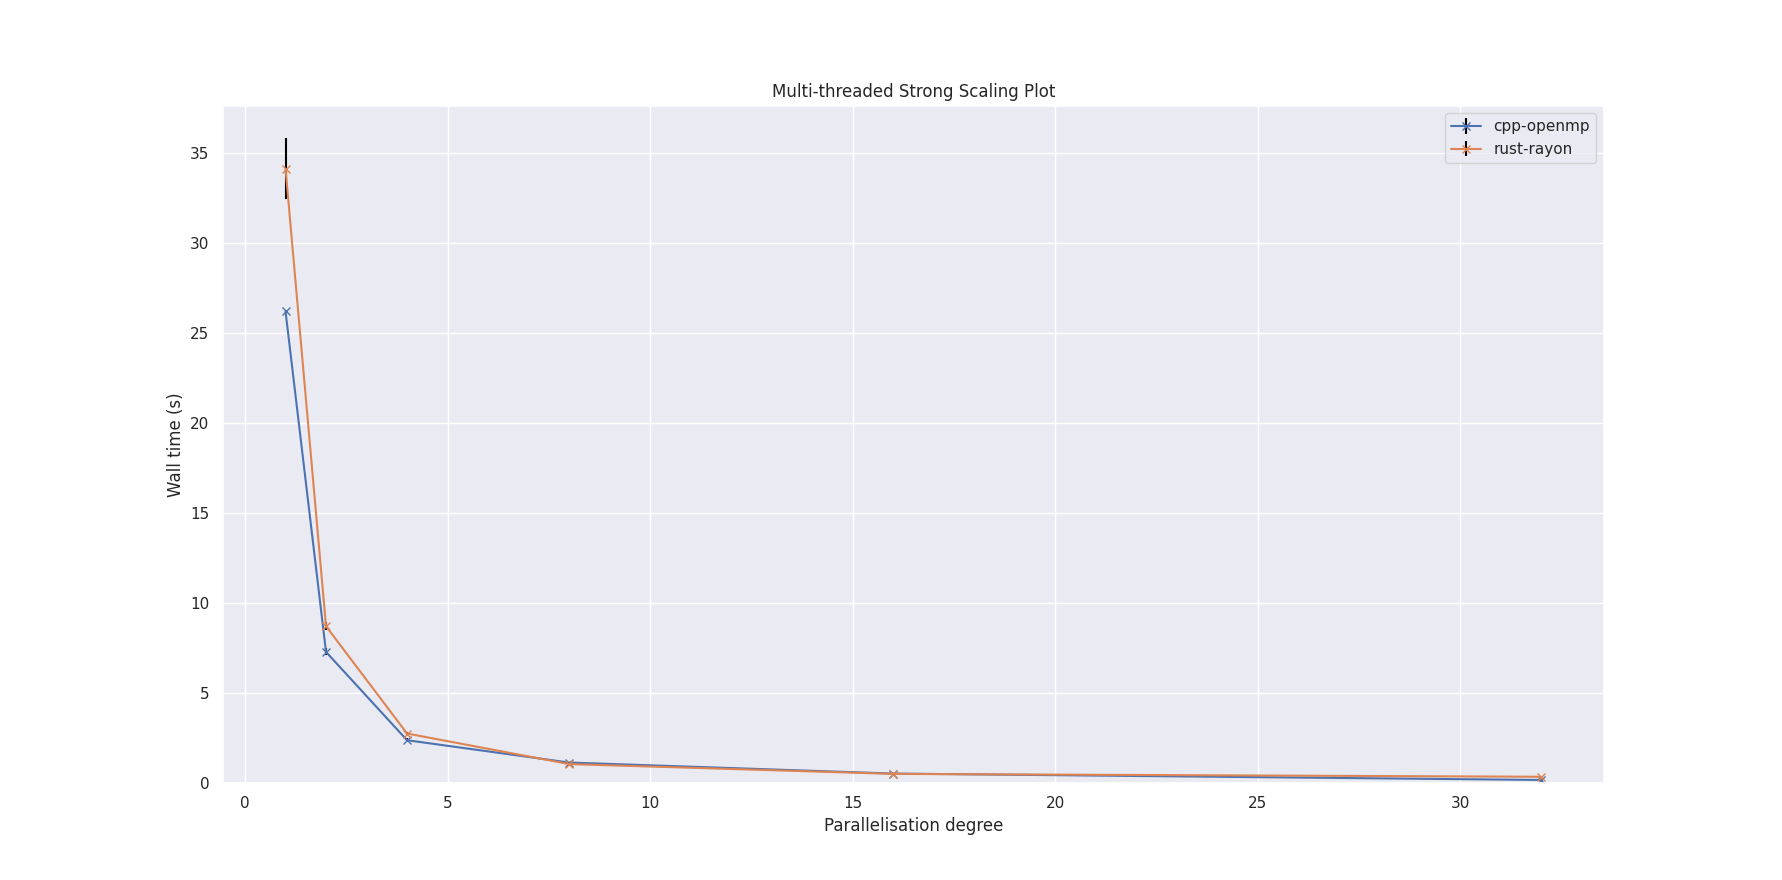
\includegraphics[width=\textwidth]{images/5_performance/scaling/strong_scaling_threaded.png}
    \caption{A line plot comparing the strong scaling runtimes of the C++ and Rust implementations of HPCCG using shared memory parallelism.}
    \label{fig:strong_scaling_threaded}
\end{figure}

\begin{figure}[H]
    \centering
    % This file was created with tikzplotlib v0.10.1.
\begin{tikzpicture}

\definecolor{darkorange25512714}{RGB}{255,127,14}
\definecolor{darkslategray38}{RGB}{38,38,38}
\definecolor{lightgray204}{RGB}{204,204,204}
\definecolor{steelblue31119180}{RGB}{31,119,180}

\begin{axis}[
axis line style={lightgray204},
height=0.45\textheight,
legend cell align={left},
legend style={fill opacity=0.8, draw opacity=1, text opacity=1, draw=none},
tick align=outside,
tick pos=left,
title={Message Passing Strong Scaling Plot},
width=\textwidth,
x grid style={lightgray204},
xlabel=\textcolor{darkslategray38}{Parallelisation degree},
xmajorgrids,
xmin=0.25, xmax=16.75,
xtick style={color=darkslategray38},
y grid style={lightgray204},
ylabel=\textcolor{darkslategray38}{Total time (s)},
ymajorgrids,
ymin=0, ymax=57.5232284677692,
ytick style={color=darkslategray38}
]
\path [draw=black, semithick]
(axis cs:1,45.8918542419206)
--(axis cs:1,46.3073457580794);

\path [draw=black, semithick]
(axis cs:2,23.0752159987937)
--(axis cs:2,23.1462340012063);

\path [draw=black, semithick]
(axis cs:4,11.5939882162363)
--(axis cs:4,11.6896117837637);

\path [draw=black, semithick]
(axis cs:8,5.84880174230194)
--(axis cs:8,5.89830825769806);

\path [draw=black, semithick]
(axis cs:16,2.94380119496893)
--(axis cs:16,2.97776880503107);

\path [draw=black, semithick]
(axis cs:1,54.5217418785546)
--(axis cs:1,54.9242081214454);

\path [draw=black, semithick]
(axis cs:2,25.506833421303)
--(axis cs:2,25.623666578697);

\path [draw=black, semithick]
(axis cs:4,12.3759604791059)
--(axis cs:4,12.4544395208941);

\path [draw=black, semithick]
(axis cs:8,6.16349884788825)
--(axis cs:8,6.86095115211175);

\path [draw=black, semithick]
(axis cs:16,3.20654452666261)
--(axis cs:16,3.21705547333739);

\addplot [semithick, steelblue31119180, mark=x, mark size=3, mark options={solid}]
table {%
1 46.0996017456055
2 23.110725402832
4 11.6417999267578
8 5.87355518341064
16 2.96078491210938
};
\addlegendentry{C++ with MPI}
\addplot [semithick, darkorange25512714, mark=x, mark size=3, mark options={solid}]
table {%
1 54.7229766845703
2 25.5652503967285
4 12.4152002334595
8 6.51222515106201
16 3.21180009841919
};
\addlegendentry{Rust with MPI}
\end{axis}

\end{tikzpicture}

    \vspace*{-0.5cm}
    % 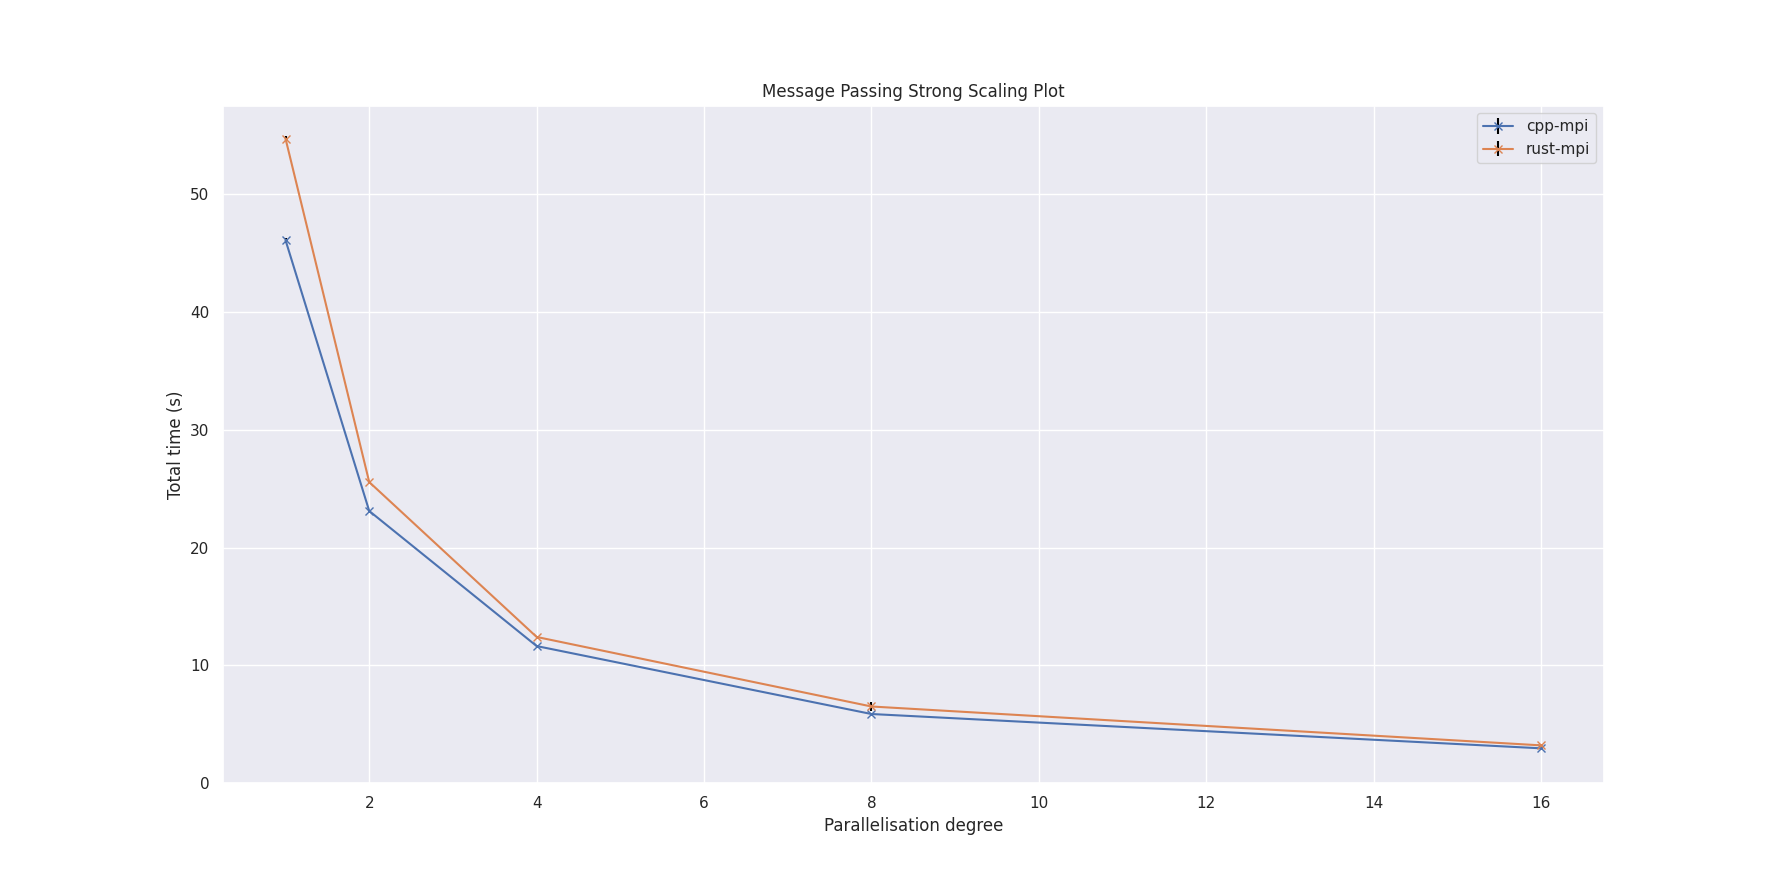
\includegraphics[width=\textwidth]{images/5_performance/scaling/strong_scaling_mpi.png}
    \caption{A line plot comparing the strong scaling speed-ups of the C++ and Rust implementations of HPCCG using distributed memory parallelism.}
    \label{fig:strong_scaling_mpi}
\end{figure}

The mesh sizes for these benchmarks are derived from testing scripts for strong scaling in the original HPCCG repository \url{https://github.com/Mantevo/HPCCG/blob/master/strongScalingRunScript}, ranging from $64 \times 64 \times 1024$ to $64 \times 64 \times 32$ reducing exponentially on the z axis. This is very surprising, as this set of inputs represents weak scaling by the above definition, but appears to exhibit the behaviour expected of strong scaling. One possible reason for this could be internal data pre-processing in preparation for splitting the mesh across MPI ranks. Investigating this peculiarity could form a good basis for future work.
% In addition to this, since these mesh sizes are small, the serial components of the computational kernels have a high impact on total performance. %These mesh sizes are comparatively small, which can be seen in the high impact of serial overhead in these results.

Leveraging the HPC MultiBench framework, we can also easily plot the speed-up of the two approaches, rather than the runtimes. The speed-up plots for the C++ and Rust implementations are shown in Figures \ref{fig:strong_scaling_speedup_threaded} and \ref{fig:strong_scaling_speedup_mpi} respectively.

\begin{figure}[H]
    \centering
    % This file was created with tikzplotlib v0.10.1.
\begin{tikzpicture}

\definecolor{darkorange25512714}{RGB}{255,127,14}
\definecolor{darkslategray38}{RGB}{38,38,38}
\definecolor{lightgray204}{RGB}{204,204,204}
\definecolor{steelblue31119180}{RGB}{31,119,180}

\begin{axis}[
axis line style={lightgray204},
height=0.4\textheight,
legend cell align={left},
legend style={
  fill opacity=0.8,
  draw opacity=1,
  text opacity=1,
  at={(0.03,0.97)},
  anchor=north west,
  % draw=none
},
tick align=outside,
tick pos=left,
title={Multi-threaded Strong Scaling Speedup Plot},
width=\textwidth,
x grid style={lightgray204},
xlabel=\textcolor{darkslategray38}{Parallelisation degree},
xmajorgrids,
xmin=-0.55, xmax=33.55,
xtick style={color=darkslategray38},
y grid style={lightgray204},
ylabel=\textcolor{darkslategray38}{Total speedup},
ymajorgrids,
ymin=0, ymax=188.083143855045,
ytick style={color=darkslategray38}
]
\path [draw=black, semithick]
(axis cs:1,1)
--(axis cs:1,1);

\path [draw=black, semithick]
(axis cs:2,3.55991378033326)
--(axis cs:2,3.7732043218572);

\path [draw=black, semithick]
(axis cs:4,11.0030411759701)
--(axis cs:4,12.0657354658402);

\path [draw=black, semithick]
(axis cs:8,23.9776565503983)
--(axis cs:8,24.4658263520519);

\path [draw=black, semithick]
(axis cs:16,52.8334845771681)
--(axis cs:16,53.5558907392404);

\path [draw=black, semithick]
(axis cs:32,165.976211774971)
--(axis cs:32,179.174422719091);

\path [draw=black, semithick]
(axis cs:1,1)
--(axis cs:1,1);

\path [draw=black, semithick]
(axis cs:2,3.7752673723536)
--(axis cs:2,4.24155251617412);

\path [draw=black, semithick]
(axis cs:4,12.2975775864902)
--(axis cs:4,13.8228237513025);

\path [draw=black, semithick]
(axis cs:8,32.9199585662537)
--(axis cs:8,37.4867683757818);

\path [draw=black, semithick]
(axis cs:16,69.3809345906386)
--(axis cs:16,77.3864702118231);

\path [draw=black, semithick]
(axis cs:32,98.7104550125276)
--(axis cs:32,109.572452036755);

\addplot [semithick, steelblue31119180, mark=x, mark size=3, mark options={solid}]
table {%
1 1
2 3.66655898094177
4 11.5343885421753
8 24.2217407226562
16 53.1946868896484
32 172.575317382812
};
\addlegendentry{C++ with OpenMP}
\addplot [semithick, darkorange25512714, mark=triangle, mark size=3, mark options={solid}]
table {%
1 1
2 4.00840997695923
4 13.0602006912231
8 35.2033653259277
16 73.3837051391602
32 104.141456604004
};
\addlegendentry{Rust with Rayon}
\end{axis}

\end{tikzpicture}

    \vspace*{-0.5cm}
    % 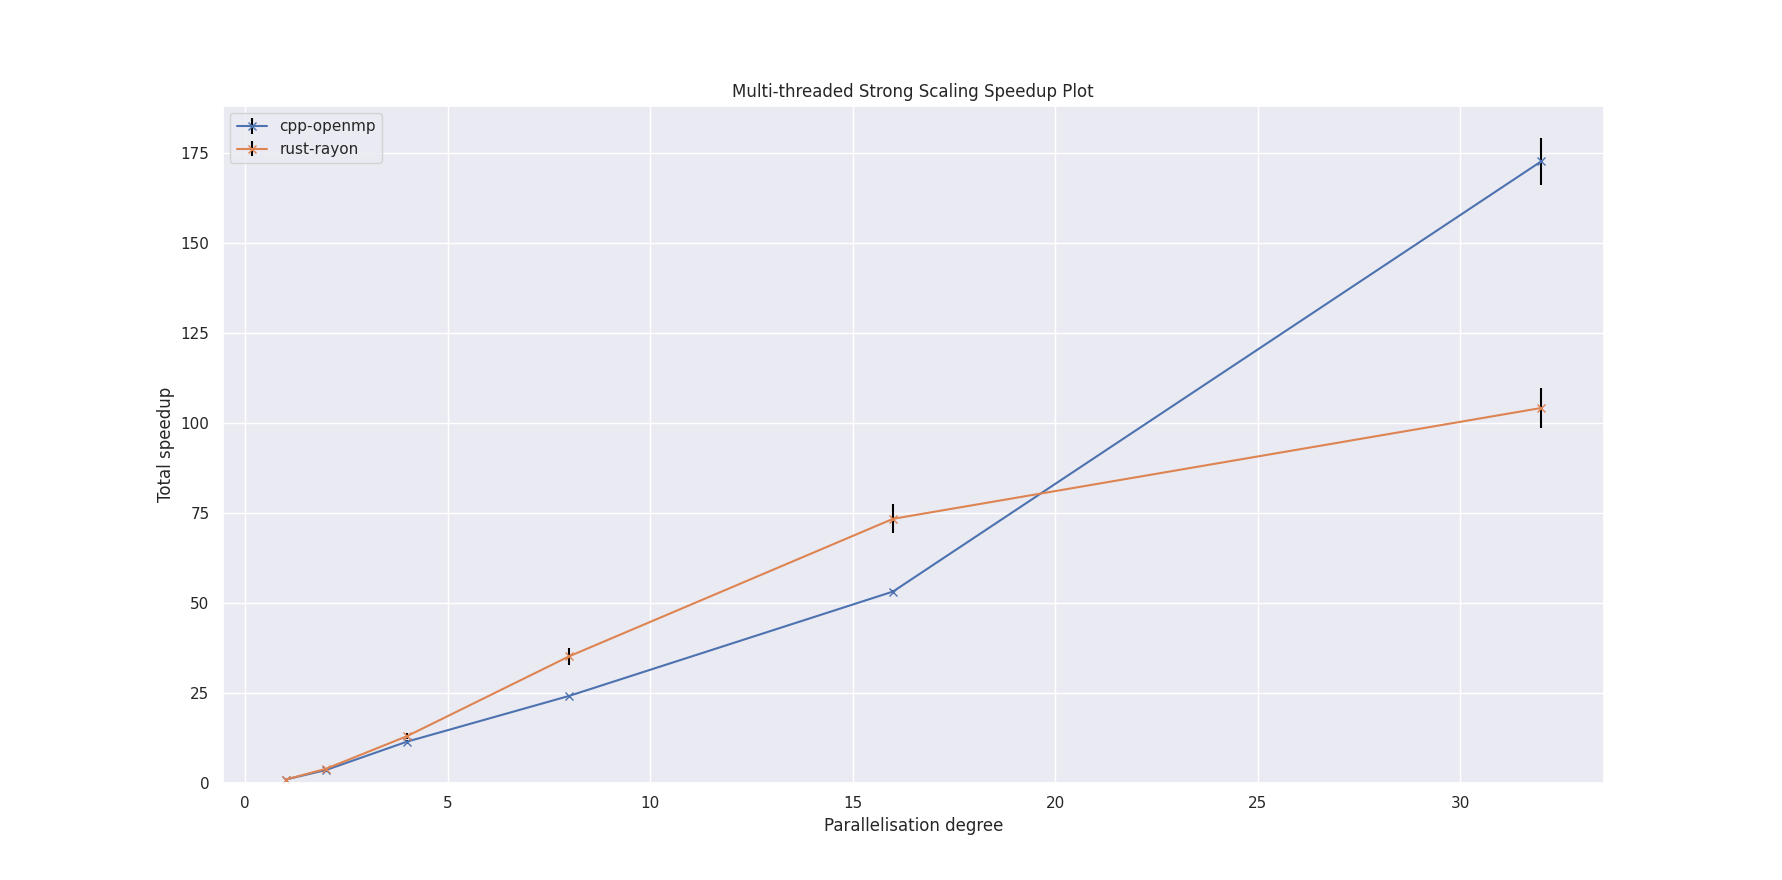
\includegraphics[width=\textwidth]{images/5_performance/scaling/strong_scaling_speedup_threaded.png}
    \caption{A line plot comparing the strong scaling speed-ups of the C++ and Rust implementations of HPCCG using shared memory parallelism.}
    \label{fig:strong_scaling_speedup_threaded}
\end{figure}

\begin{figure}[H]
    \centering
    % This file was created with tikzplotlib v0.10.1.
\begin{tikzpicture}

\definecolor{darkorange25512714}{RGB}{255,127,14}
\definecolor{darkslategray38}{RGB}{38,38,38}
\definecolor{lightgray204}{RGB}{204,204,204}
\definecolor{steelblue31119180}{RGB}{31,119,180}

\begin{axis}[
axis line style={lightgray204},
height=0.4\textheight,
legend cell align={left},
legend style={
  fill opacity=0.8,
  draw opacity=1,
  text opacity=1,
  at={(0.03,0.97)},
  anchor=north west,
  % draw=none
},
tick align=outside,
tick pos=left,
title={Message Passing Strong Scaling Speedup Plot},
width=\textwidth,
x grid style={lightgray204},
xlabel=\textcolor{darkslategray38}{Parallelisation degree},
xmajorgrids,
xmin=0.25, xmax=16.75,
xtick style={color=darkslategray38},
y grid style={lightgray204},
ylabel=\textcolor{darkslategray38}{Total speedup},
ymajorgrids,
ymin=0, ymax=17.9120127975498,
ytick style={color=darkslategray38}
]
\path [draw=black, semithick]
(axis cs:1,1)
--(axis cs:1,1);

\path [draw=black, semithick]
(axis cs:2,1.9852302892385)
--(axis cs:2,2.00422482305243);

\path [draw=black, semithick]
(axis cs:4,3.93569082317226)
--(axis cs:4,3.9839779565697);

\path [draw=black, semithick]
(axis cs:8,7.80024454067345)
--(axis cs:8,7.89709718848377);

\path [draw=black, semithick]
(axis cs:16,15.4564809891002)
--(axis cs:16,15.6836389453091);

\path [draw=black, semithick]
(axis cs:1,1)
--(axis cs:1,1);

\path [draw=black, semithick]
(axis cs:2,2.13125460310141)
--(axis cs:2,2.14978900100964);

\path [draw=black, semithick]
(axis cs:4,4.38636734496599)
--(axis cs:4,4.42911287283155);

\path [draw=black, semithick]
(axis cs:8,7.9520728687921)
--(axis cs:8,8.85415695281265);

\path [draw=black, semithick]
(axis cs:16,16.9695245202452)
--(axis cs:16,17.1066788548093);

\addplot [semithick, steelblue31119180, mark=x, mark size=3, mark options={solid}]
table {%
1 1
2 1.99472761154175
4 3.9598343372345
8 7.84867095947266
16 15.5700597763062
};
\addlegendentry{C++ with MPI}
\addplot [semithick, darkorange25512714, mark=triangle, mark size=3, mark options={solid}]
table {%
1 1
2 2.14052176475525
4 4.40774011611938
8 8.40311527252197
16 17.0381011962891
};
\addlegendentry{Rust with MPI}
\end{axis}

\end{tikzpicture}

    \vspace*{-0.5cm}
    % 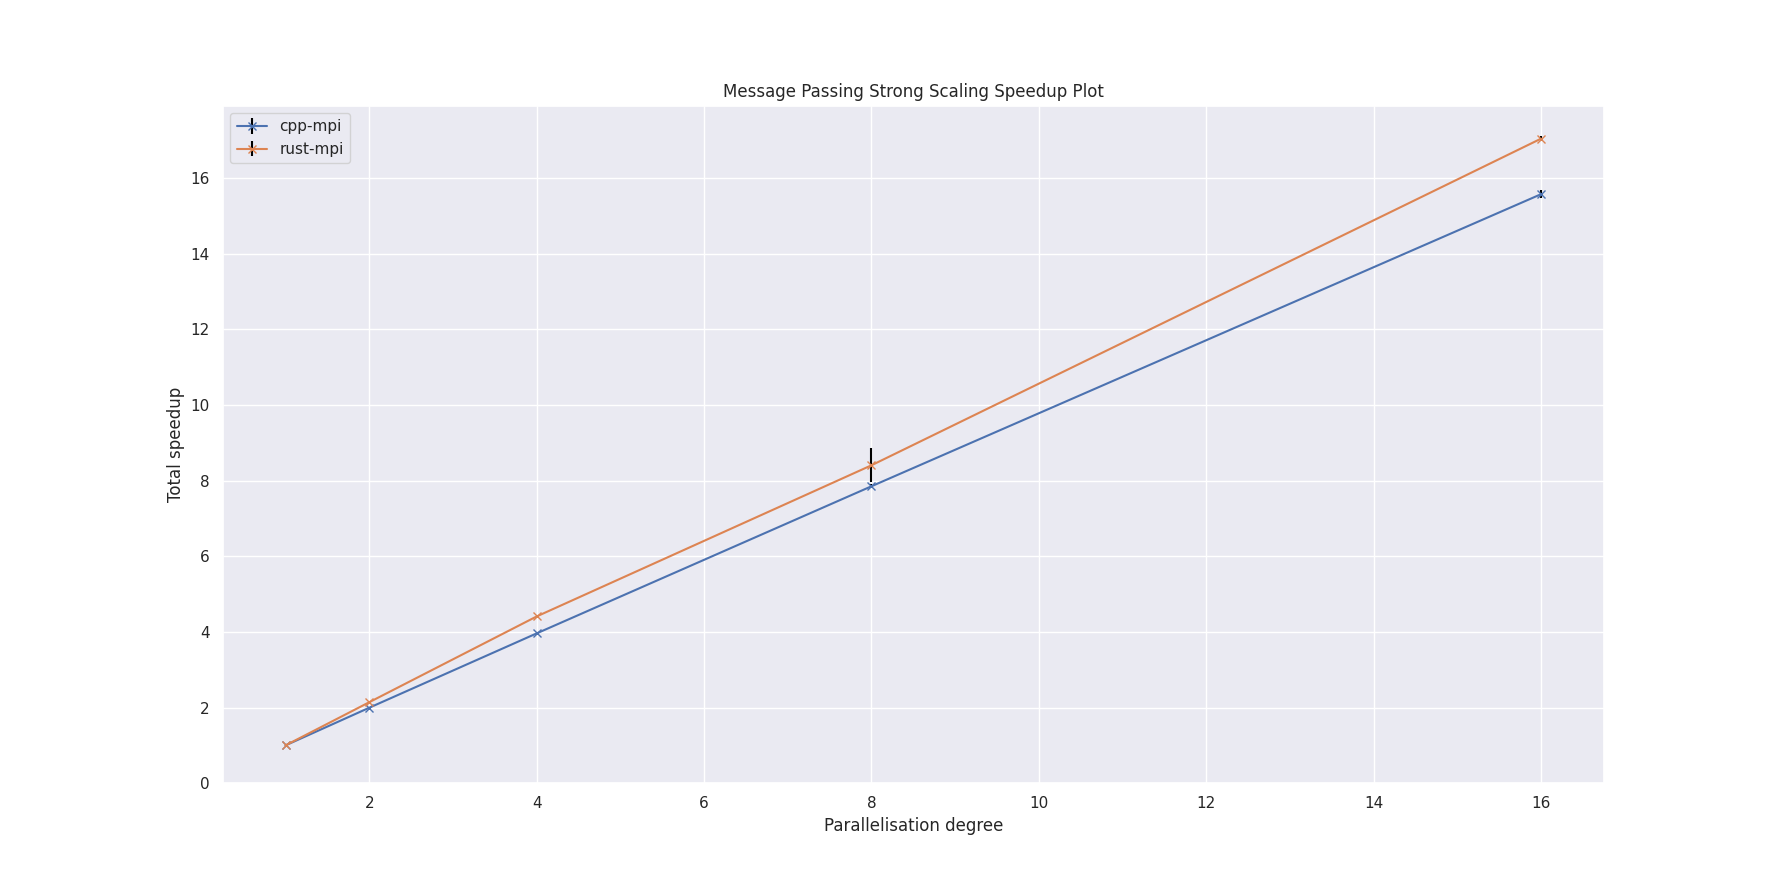
\includegraphics[width=\textwidth]{images/5_performance/scaling/strong_scaling_speedup_mpi.png}
    \caption{A line plot comparing the strong scaling runtimes of the C++ and Rust implementations of HPCCG using distributed memory parallelism.}
    \label{fig:strong_scaling_speedup_mpi}
\end{figure}

Examining the plots showing speed-up rather than runtime allow better understanding of the trends in program performance. From these speed-up plots, we can see that for the small meshes tested, Rust's threading model through Rayon of work stealing appears to scale less well than OpenMP, outside the range of experimental error. However, this is likely due to the significant impact the serial overhead of setting up the thread pool has on the total execution time for such small workloads. For MPI, we can see an almost ideal strong scaling speed-up of two very straight lines. Again, the speed-up of Rust is slightly lower, which is likely due to overhead incurred in invoking the MPI bindings.

In summary, we can see that both the C++ and Rust implementations strongly scale similarly, with both being close to the theoretical limitation of Amdahl's law. This evidence of similar strong scalability provides confidence in the suitability of Rust for High-Performance Computing workloads, which require this property to effectively leverage clustered compute resources.

\subsection{Weak scaling}
\label{ssec:weak-scaling}

Patterson and Hennessy define weak scaling as when ``the problem size grows proportionally to the increase in the number of processors'' \cite{pattersonHennessyComputerOrganisationArchitecture}. This can be characterised by recording the wall clock time taken, whilst varying the problem size at the same rate as the varying the degree of parallelisation. Since the workload grows with the number of resources added, ideal weak scaling is when the execution time remains constant as both factors are increased.

Unlike strong scaling, we cannot apply Amdahl's law to characterise weak scaling, since it assumes a fixed problem size. However, this extended case of variable problem size was characterised in Gustafson's 1988 paper ``Re-evaluating Amdahl's law'' \cite{gustafsonReevaluatingAmdahlLaw1988}. Gustafson's law estimates the speed-up, $S$ as a result of parallelisation in terms of the number of processors $N$, and the fractions of time executing the parallel and serial parts of the program, $p$ and $s$ respectively:

\begin{align}
    S &= s + p \times N \\
      &= N + (1 - N) \times s
\end{align}

From the above equation, we can see that for ideal weak scaling to occur, the serial component of the program must remain constant as the degree of parallelism is increased. In real-world applications, we expect this to not be the case, as higher degrees of parallelism often incur higher serial costs, such as handling increased communication for MPI workloads, or overhead from spawning threads for multithreaded ones.

As with strong scaling, weak scaling can be assessed for both parallelism approaches in the context of the HPCCG mini-app. Figures \ref{fig:weak_scaling_threaded} and \ref{fig:weak_scaling_mpi} compare the weak scaling characteristics of the total runtimes of the C++ and Rust implementations. The mesh sizes for these benchmarks are again derived from testing scripts for weak scaling in the original HPCCG repository, with the problem size fixed as $64 \times 64 \times 64$.

% TODO: Could cut raw runtime plots if they aren't interesting?
\begin{figure}[H]
    \centering
    % This file was created with tikzplotlib v0.10.1.
\begin{tikzpicture}

\definecolor{darkorange25512714}{RGB}{255,127,14}
\definecolor{darkslategray38}{RGB}{38,38,38}
\definecolor{lightgray204}{RGB}{204,204,204}
\definecolor{steelblue31119180}{RGB}{31,119,180}

\begin{axis}[
axis line style={lightgray204},
height=0.45\textheight,
legend cell align={left},
legend style={fill opacity=0.8, draw opacity=1, text opacity=1, draw=none},
tick align=outside,
tick pos=left,
title={Multi-threaded Weak Scaling Plot},
width=\textwidth,
x grid style={lightgray204},
xlabel=\textcolor{darkslategray38}{Parallelisation degree},
xmajorgrids,
xmin=-0.55, xmax=33.55,
xtick style={color=darkslategray38},
y grid style={lightgray204},
ylabel=\textcolor{darkslategray38}{Wall time (s)},
ymajorgrids,
ymin=0, ymax=1.86548483460824,
ytick style={color=darkslategray38}
]
\path [draw=black, semithick]
(axis cs:1,1.63208456608574)
--(axis cs:1,1.77291543391426);

\path [draw=black, semithick]
(axis cs:2,0.929226497308104)
--(axis cs:2,0.940773502691896);

\path [draw=black, semithick]
(axis cs:4,0.681835034190723)
--(axis cs:4,0.698164965809277);

\path [draw=black, semithick]
(axis cs:8,0.5725)
--(axis cs:8,0.5825);

\path [draw=black, semithick]
(axis cs:16,0.53)
--(axis cs:16,0.53);

\path [draw=black, semithick]
(axis cs:32,0.6125)
--(axis cs:32,0.6225);

\path [draw=black, semithick]
(axis cs:1,1.64445087017355)
--(axis cs:1,1.80054912982645);

\path [draw=black, semithick]
(axis cs:2,1.04189724227463)
--(axis cs:2,1.15310275772537);

\path [draw=black, semithick]
(axis cs:4,0.814337719488098)
--(axis cs:4,0.915662280511902);

\path [draw=black, semithick]
(axis cs:8,0.542084267568224)
--(axis cs:8,0.727915732431776);

\path [draw=black, semithick]
(axis cs:16,0.501835034190723)
--(axis cs:16,0.518164965809277);

\path [draw=black, semithick]
(axis cs:32,0.569226497308104)
--(axis cs:32,0.580773502691896);

\addplot [semithick, steelblue31119180, mark=x, mark size=3, mark options={solid}]
table {%
1 1.70249998569489
2 0.934999942779541
4 0.690000057220459
8 0.577499985694885
16 0.529999971389771
32 0.617500066757202
};
\addlegendentry{C++ with OpenMP}
\addplot [semithick, darkorange25512714, mark=x, mark size=3, mark options={solid}]
table {%
1 1.7224999666214
2 1.0974999666214
4 0.865000009536743
8 0.634999990463257
16 0.509999990463257
32 0.575000047683716
};
\addlegendentry{Rust with Rayon}
\end{axis}

\end{tikzpicture}

    \vspace*{-0.5cm}
    % 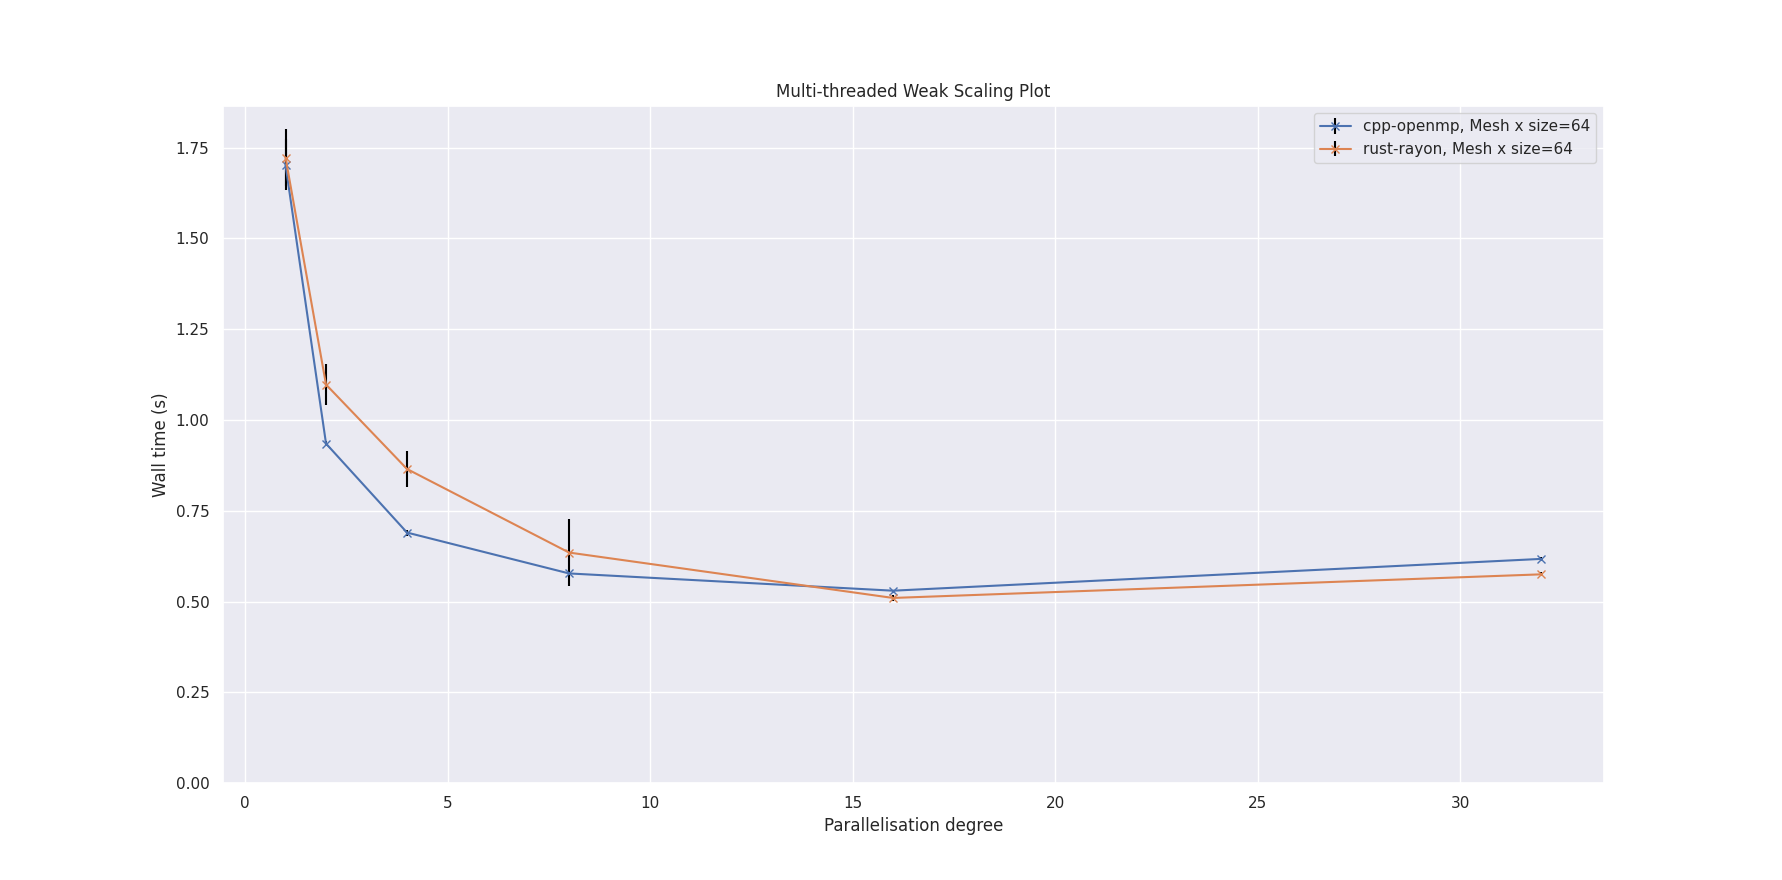
\includegraphics[width=\textwidth]{images/5_performance/scaling/weak_scaling_threaded.png}
    \caption{A line plot comparing the weak scaling runtimes of the C++ and Rust implementations of HPCCG using shared memory parallelism.}
    \label{fig:weak_scaling_threaded}
\end{figure}

\begin{figure}[H]
    \centering
    % This file was created with tikzplotlib v0.10.1.
\begin{tikzpicture}

\definecolor{darkorange25512714}{RGB}{255,127,14}
\definecolor{darkslategray38}{RGB}{38,38,38}
\definecolor{lightgray204}{RGB}{204,204,204}
\definecolor{steelblue31119180}{RGB}{31,119,180}

\begin{axis}[
axis line style={lightgray204},
height=0.45\textheight,
legend cell align={left},
legend style={fill opacity=0.8, draw opacity=1, text opacity=1, draw=none},
tick align=outside,
tick pos=left,
title={Message Passing Weak Scaling Plot},
width=\textwidth,
x grid style={lightgray204},
xlabel=\textcolor{darkslategray38}{Parallelisation degree},
xmajorgrids,
xmin=0.25, xmax=16.75,
xtick style={color=darkslategray38},
y grid style={lightgray204},
ylabel=\textcolor{darkslategray38}{Total time (s)},
ymajorgrids,
ymin=0, ymax=5,
ytick style={color=darkslategray38}
]
\path [draw=black, semithick]
(axis cs:1,2.94000165222455)
--(axis cs:1,2.97673834777545);

\path [draw=black, semithick]
(axis cs:2,2.95137182427439)
--(axis cs:2,2.95688817572561);

\path [draw=black, semithick]
(axis cs:4,2.93446971279441)
--(axis cs:4,2.95980028720559);

\path [draw=black, semithick]
(axis cs:8,2.95429760952029)
--(axis cs:8,2.96441739047971);

\path [draw=black, semithick]
(axis cs:16,2.94183241809302)
--(axis cs:16,2.96462258190697);

\path [draw=black, semithick]
(axis cs:1,3.21015660196518)
--(axis cs:1,3.22299339803482);

\path [draw=black, semithick]
(axis cs:2,3.20870843824999)
--(axis cs:2,3.22724156175001);

\path [draw=black, semithick]
(axis cs:4,3.22015421748723)
--(axis cs:4,3.22049578251277);

\path [draw=black, semithick]
(axis cs:8,3.21797331132462)
--(axis cs:8,3.22352668867538);

\path [draw=black, semithick]
(axis cs:16,3.18956361077749)
--(axis cs:16,3.21708638922251);

\addplot [semithick, steelblue31119180, mark=x, mark size=3, mark options={solid}]
table {%
1 2.95836997032166
2 2.95412993431091
4 2.94713497161865
8 2.95935750007629
16 2.95322751998901
};
\addlegendentry{C++ with MPI}
\addplot [semithick, darkorange25512714, mark=x, mark size=3, mark options={solid}]
table {%
1 3.21657490730286
2 3.21797490119934
4 3.22032499313354
8 3.22075009346008
16 3.20332503318787
};
\addlegendentry{Rust with MPI}
\end{axis}

\end{tikzpicture}

    \vspace*{-0.5cm}
    % 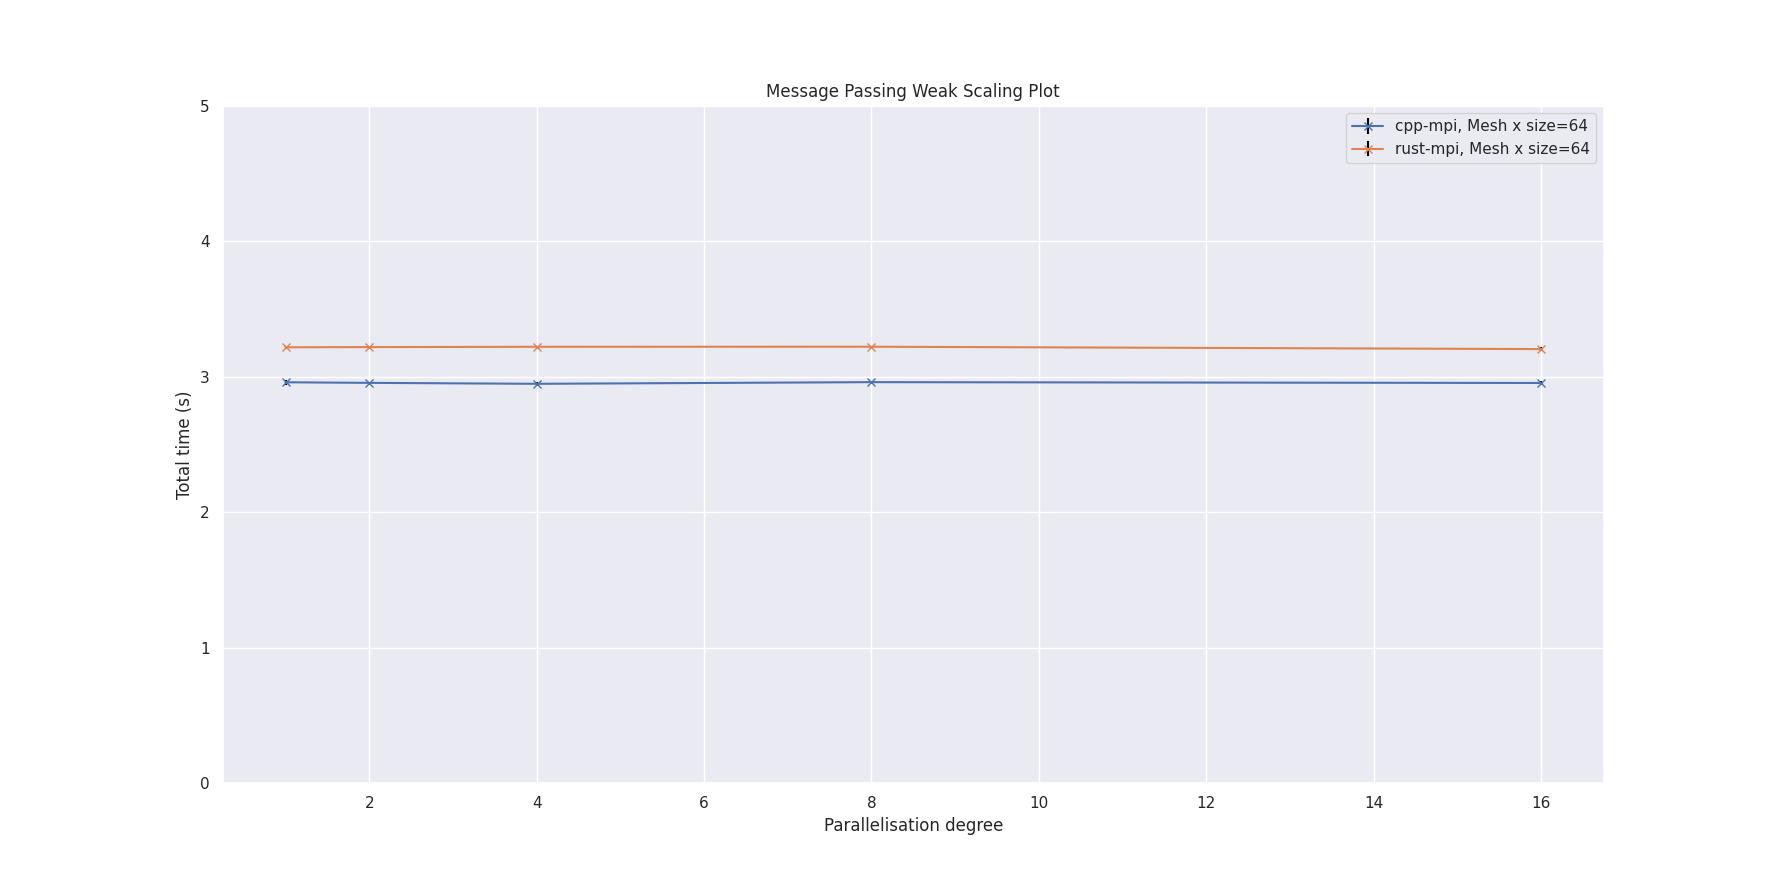
\includegraphics[width=\textwidth]{images/5_performance/scaling/weak_scaling_mpi.png}
    \caption{A line plot comparing the weak scaling speed-ups of the C++ and Rust implementations of HPCCG using distributed memory parallelism.}
    \label{fig:weak_scaling_mpi}
\end{figure}

Again, we can leverage the HPC MultiBench framework to plot the speed-up of the two approaches, rather than the runtimes. The speed-up plots for the C++ and Rust implementations are shown in Figures \ref{fig:weak_scaling_speedup_threaded} and \ref{fig:weak_scaling_speedup_mpi} respectively.

\begin{figure}[H]
    \centering
    % This file was created with tikzplotlib v0.10.1.
\begin{tikzpicture}

\definecolor{darkorange25512714}{RGB}{255,127,14}
\definecolor{darkslategray38}{RGB}{38,38,38}
\definecolor{lightgray204}{RGB}{204,204,204}
\definecolor{steelblue31119180}{RGB}{31,119,180}

\begin{axis}[
axis line style={lightgray204},
height=0.45\textheight,
legend cell align={left},
legend style={
  fill opacity=0.8,
  draw opacity=1,
  text opacity=1,
  at={(0.03,0.03)},
  anchor=south west,
  draw=none
},
tick align=outside,
tick pos=left,
title={Multi-threaded Weak Scaling Speedup Plot},
width=\textwidth,
x grid style={lightgray204},
xlabel=\textcolor{darkslategray38}{Parallelisation degree},
xmajorgrids,
xmin=-0.55, xmax=33.55,
xtick style={color=darkslategray38},
y grid style={lightgray204},
ylabel=\textcolor{darkslategray38}{Total speedup},
ymajorgrids,
ymin=0, ymax=3.95739220158455,
ytick style={color=darkslategray38}
]
\path [draw=black, semithick]
(axis cs:1,1)
--(axis cs:1,1);

\path [draw=black, semithick]
(axis cs:2,1.79175187821461)
--(axis cs:2,1.94976184556382);

\path [draw=black, semithick]
(axis cs:4,2.47404798404419)
--(axis cs:4,2.69465521766648);

\path [draw=black, semithick]
(axis cs:8,2.99442959552332)
--(axis cs:8,3.25909725024797);

\path [draw=black, semithick]
(axis cs:16,3.28021521050717)
--(axis cs:16,3.56946769090078);

\path [draw=black, semithick]
(axis cs:32,2.80345922910994)
--(axis cs:32,3.05425726227466);

\path [draw=black, semithick]
(axis cs:1,1)
--(axis cs:1,1);

\path [draw=black, semithick]
(axis cs:2,1.47929800414883)
--(axis cs:2,1.70150513942027);

\path [draw=black, semithick]
(axis cs:4,1.8850407871372)
--(axis cs:4,2.24493681365922);

\path [draw=black, semithick]
(axis cs:8,2.3783530404398)
--(axis cs:8,3.30144843990076);

\path [draw=black, semithick]
(axis cs:16,3.45125599192132)
--(axis cs:16,3.8165640015091);

\path [draw=black, semithick]
(axis cs:32,3.03354699492063)
--(axis cs:32,3.3344675875133);

\addplot [semithick, steelblue31119180, mark=x, mark size=3, mark options={solid}]
table {%
1 1
2 1.87075686454773
4 2.58435153961182
8 3.12676334381104
16 3.42484140396118
32 2.92885828018188
};
\addlegendentry{C++ with OpenMP}
\addplot [semithick, darkorange25512714, mark=x, mark size=3, mark options={solid}]
table {%
1 1
2 1.59040153026581
4 2.06498885154724
8 2.83990073204041
16 3.6339099407196
32 3.18400740623474
};
\addlegendentry{Rust with Rayon}
\end{axis}

\end{tikzpicture}

    \vspace*{-0.5cm}
    % 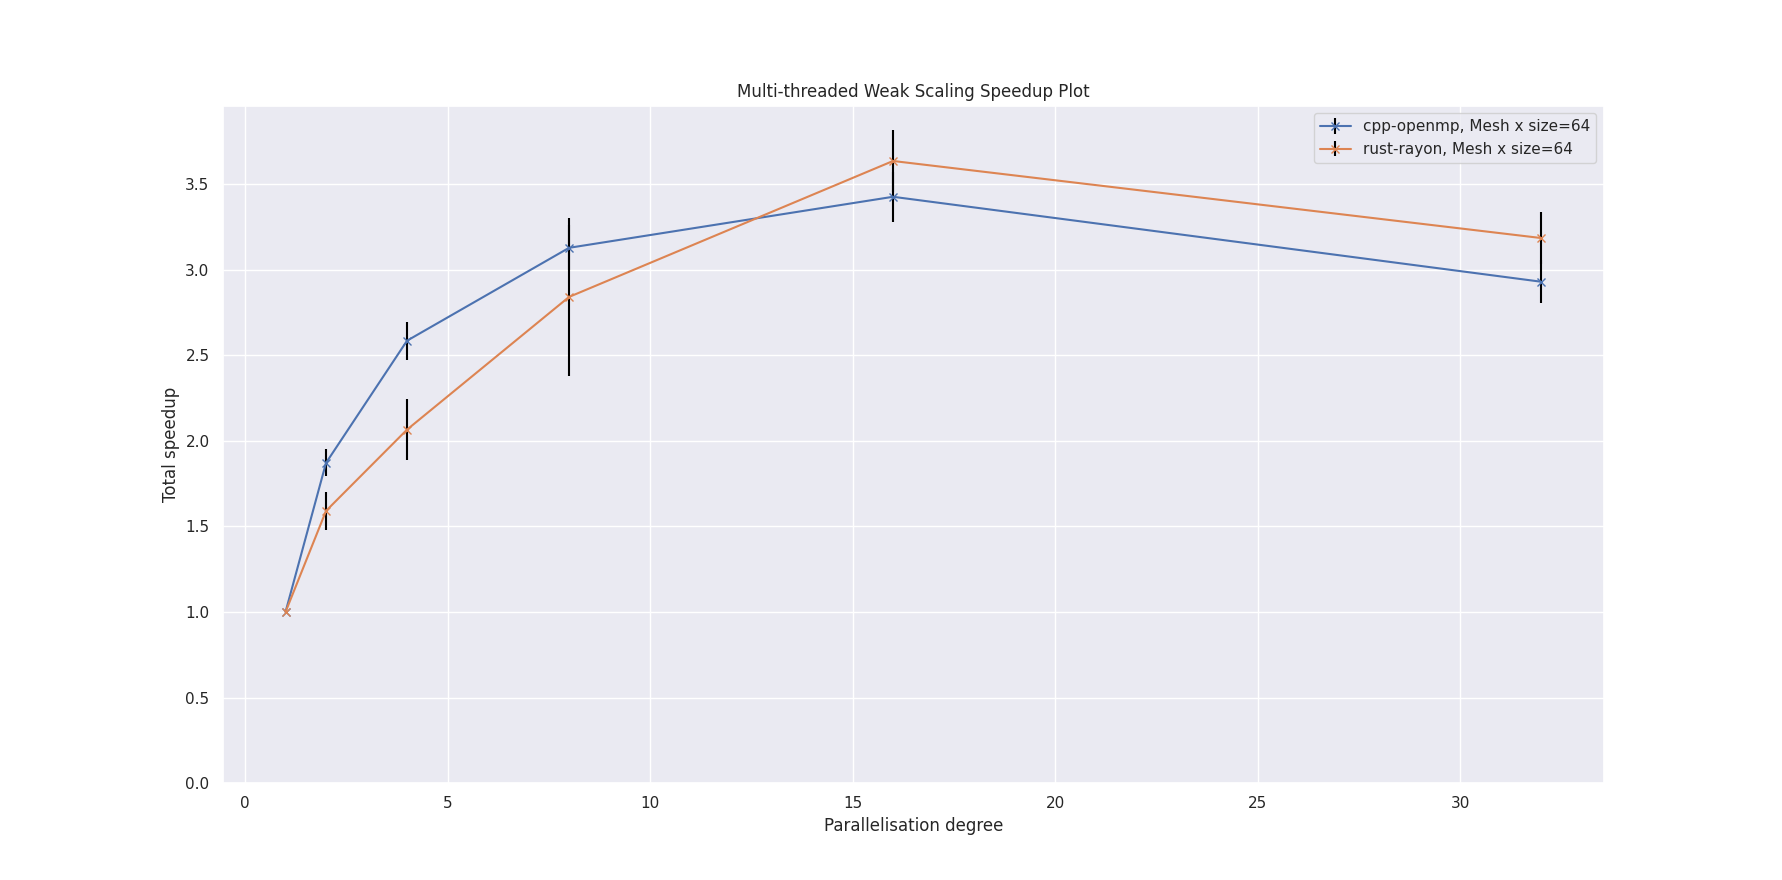
\includegraphics[width=\textwidth]{images/5_performance/scaling/weak_scaling_speedup_threaded.png}
    \caption{A line plot comparing the weak scaling speed-ups of the C++ and Rust implementations of HPCCG using shared memory parallelism.}
    \label{fig:weak_scaling_speedup_threaded}
\end{figure}

\begin{figure}[H]
    \centering
    % This file was created with tikzplotlib v0.10.1.
\begin{tikzpicture}

\definecolor{darkorange25512714}{RGB}{255,127,14}
\definecolor{darkslategray38}{RGB}{38,38,38}
\definecolor{lightgray204}{RGB}{204,204,204}
\definecolor{steelblue31119180}{RGB}{31,119,180}

\begin{axis}[
axis line style={lightgray204},
height=0.45\textheight,
legend cell align={left},
legend style={fill opacity=0.8, draw opacity=1, text opacity=1, draw=none},
tick align=outside,
tick pos=left,
title={Message Passing Weak Scaling Speedup Plot},
width=\textwidth,
x grid style={lightgray204},
xlabel=\textcolor{darkslategray38}{Parallelisation degree},
xmajorgrids,
xmin=0.25, xmax=16.75,
xtick style={color=darkslategray38},
y grid style={lightgray204},
ylabel=\textcolor{darkslategray38}{Total speedup},
ymajorgrids,
ymin=0.9, ymax=1.1,
ytick style={color=darkslategray38}
]
\path [draw=black, semithick]
(axis cs:1,1)
--(axis cs:1,1);

\path [draw=black, semithick]
(axis cs:2,0.995147517413405)
--(axis cs:2,1.00772304007729);

\path [draw=black, semithick]
(axis cs:4,0.996232272058601)
--(axis cs:4,1.01139208176299);

\path [draw=black, semithick]
(axis cs:8,0.993228403052343)
--(axis cs:8,1.00610422235706);

\path [draw=black, semithick]
(axis cs:16,0.994418379065732)
--(axis cs:16,1.00906425137842);

\path [draw=black, semithick]
(axis cs:1,1)
--(axis cs:1,1);

\path [draw=black, semithick]
(axis cs:2,0.996063052909887)
--(axis cs:2,1.0030668346747);

\path [draw=black, semithick]
(axis cs:4,0.996841727322463)
--(axis cs:4,1.00082931519654);

\path [draw=black, semithick]
(axis cs:8,0.996532844145171)
--(axis cs:8,1.000874592011);

\path [draw=black, semithick]
(axis cs:16,0.999379959252298)
--(axis cs:16,1.00889269494295);

\addplot [semithick, steelblue31119180, mark=x, mark size=3, mark options={solid}]
table {%
1 1
2 1.00143527984619
4 1.00381219387054
8 0.999666333198547
16 1.00174129009247
};
\addlegendentry{C++ with MPI}
\addplot [semithick, darkorange25512714, mark=x, mark size=3, mark options={solid}]
table {%
1 1
2 0.99956488609314
4 0.998835563659668
8 0.998703718185425
16 1.00413632392883
};
\addlegendentry{Rust with MPI}
\end{axis}

\end{tikzpicture}

    \vspace*{-0.5cm}
    % 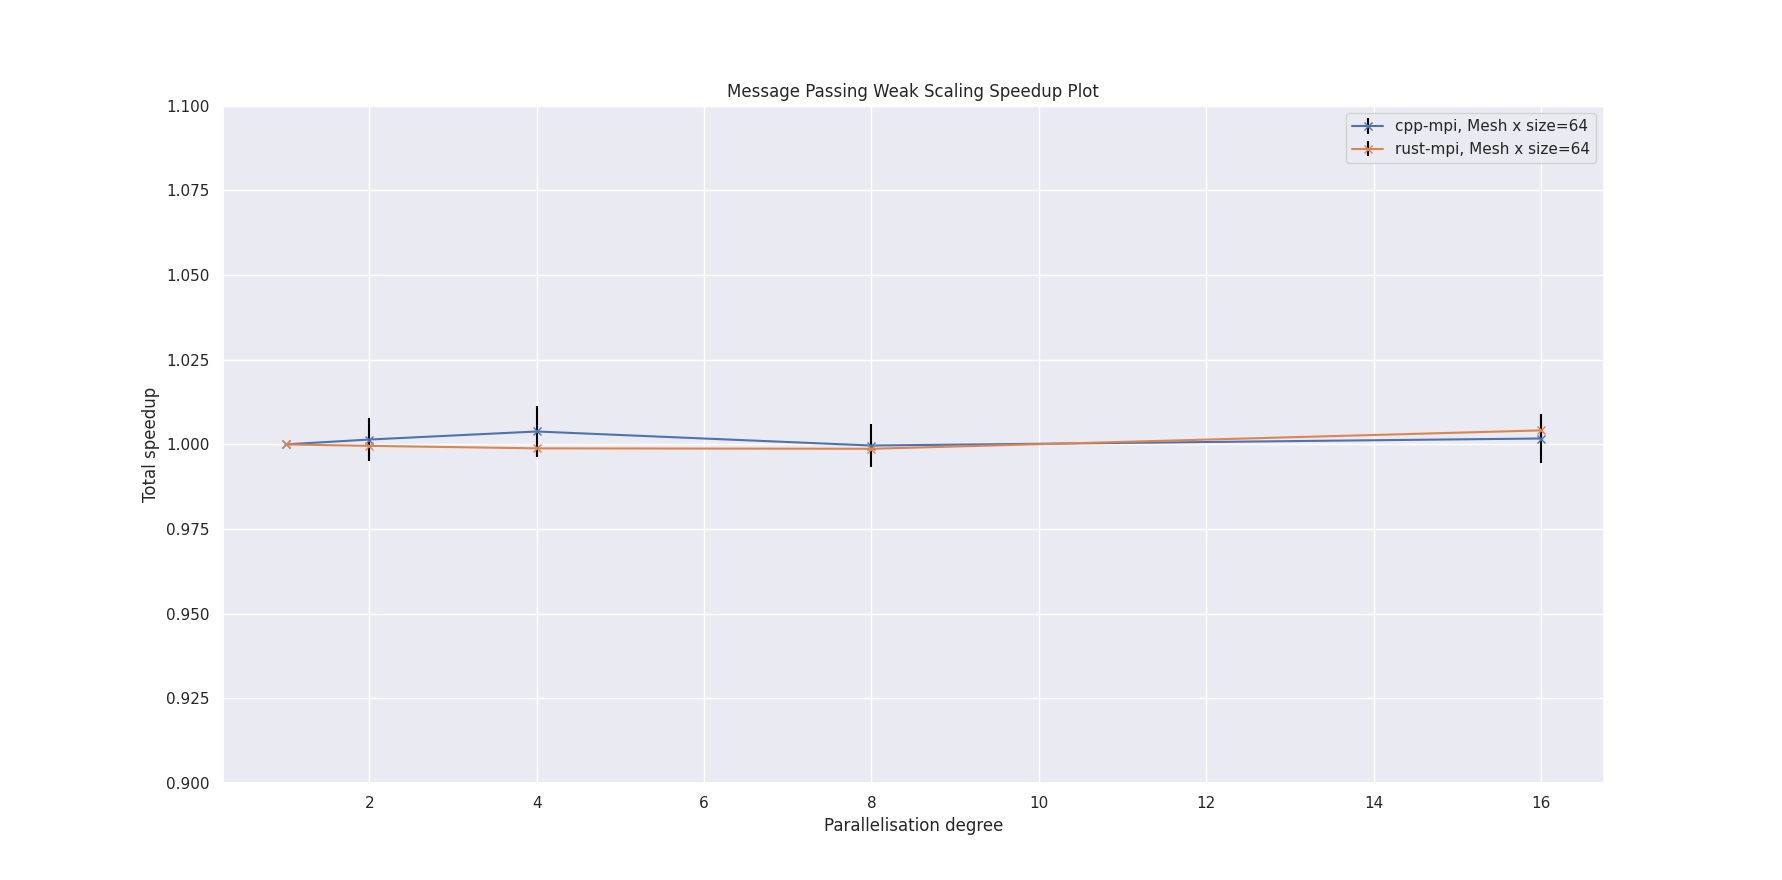
\includegraphics[width=\textwidth]{images/5_performance/scaling/weak_scaling_speedup_mpi.png}
    \caption{A line plot comparing the weak scaling runtimes of the C++ and Rust implementations of HPCCG using distributed memory parallelism.}
    \label{fig:weak_scaling_speedup_mpi}
\end{figure}

As with strong scaling, the speed-up plots most effectively show the trends in program performance. The weak scaling trends of the multithreaded approach are surprising, as the ideal result is a flat line, as seen in the message passing approach. The initial upwards trend in speed-up for the multithreaded approach is likely because the serial overhead of setting up threading for very small thread counts dominates the runtime for small meshes, as a corollary of Amdahl's law. The speed-up then trends back down for high thread counts, which could be due to the mesh being insufficiently large to effectively divide work between the threads.

The weak scaling speed-up of the message passing approach is very consistent across the two languages, with the Rust and C++ implementations being within experimental uncertainty of each other. This is likely because Rust is invoking the same MPI implementation that C++ uses, albeit through foreign-function interface bindings.

In summary, we can see that both the C++ and Rust implementations weakly scale similarly, with both parallelism approaches following the same trends across the languages. This evidence of similar weak scalability again provides confidence in the suitability of Rust for High-Performance Computing workloads, which require this property to effectively leverage clustered compute resources.




\subsection{Parallelism approaches}
\label{ssec:parallelism-approaches}

% TODO: cite (same as background)
In modern High-Performance Computing systems, the majority of performance is achieved through parallelism, as predicted by the Mantevo Suite paper \cite{heroux2013mantevo}. As a result of this, for Rust to be suitable for use in High-Performance Computing workloads, it must be able to achieve parallel compute performance similar to that of currently used languages such as C++. This section provides an empirical analysis of the performance of Rust as compared with C++ for increasingly parallel workloads, from serial as a reference to shared memory parallelism through multi-threading and distributed memory parallelism through message passing.

\subsection{Serial execution}
\label{ssec:serial-execution}

For many workloads, overall performance is bottlenecked by their serial components. This is because almost any program leveraging parallelism will have serial sections, and even if these are very short they can take up a significant proportion of a program's runtime for highly parallel programs, as a corollary of Amdahl's law \cite{amdahlsLaw}. As such, measuring serial performance is a critical component of the overall assessment of Rust's performance in High-Performance Computing applications.

To assess serial performance, we ran the C++ and Rust executables over a range of mesh sizes, from $100 \times 100 \times 100$ to $300 \times 300 \times 300$, incrementing each axis size by $50$ each time. We expect the performance to scale with the total size of the mesh, which is the produce of the edge sizes. In addition to the experimental methodology discussed in section \ref{ssec:experimental-methodology}, all serial runs were conducted on a single node in the compute cluster, with a single task per node, and exclusive use of that node to reduce machine noise from other processes.

\begin{figure}[H]
    \centering
    % This file was created with tikzplotlib v0.10.1.
\begin{tikzpicture}

\definecolor{darkorange25512714}{RGB}{255,127,14}
\definecolor{darkslategray38}{RGB}{38,38,38}
\definecolor{lightgray204}{RGB}{204,204,204}
\definecolor{steelblue31119180}{RGB}{31,119,180}

\begin{axis}[
axis line style={lightgray204},
height=0.375\textheight,
legend cell align={left},
legend style={
  fill opacity=0.8,
  draw opacity=1,
  text opacity=1,
  at={(0.03,0.97)},
  anchor=north west,
  % draw=none
},
tick align=outside,
tick pos=left,
title={Serial Implementation Comparison},
width=\textwidth,
x grid style={lightgray204},
xlabel=\textcolor{darkslategray38}{Mesh size},
xmajorgrids,
xmin=-300000, xmax=28300000,
xtick style={color=darkslategray38},
xtick={-5000000,0,5000000,10000000,15000000,20000000,25000000,30000000},
xticklabels={\ensuremath{-}0.5,0.0,0.5,1.0,1.5,2.0,2.5,3.0},
y grid style={lightgray204},
ylabel=\textcolor{darkslategray38}{Total time (s)},
ymajorgrids,
ymin=-4.37112772742832, ymax=207.278019459855,
ytick style={color=darkslategray38}
]
\path [draw=black, semithick]
(axis cs:1000000,5.24928805381182)
--(axis cs:1000000,5.38093194618818);

\path [draw=black, semithick]
(axis cs:3375000,18.2362775143149)
--(axis cs:3375000,18.5918224856851);

\path [draw=black, semithick]
(axis cs:8000000,43.0112248050381)
--(axis cs:8000000,44.2646751949619);

\path [draw=black, semithick]
(axis cs:15625000,83.8727643552916)
--(axis cs:15625000,86.8532856447084);

\path [draw=black, semithick]
(axis cs:27000000,145.22678151586)
--(axis cs:27000000,150.04971848414);

\path [draw=black, semithick]
(axis cs:1000000,6.06501455484037)
--(axis cs:1000000,6.20378544515963);

\path [draw=black, semithick]
(axis cs:3375000,21.7123181805685)
--(axis cs:3375000,21.9782318194315);

\path [draw=black, semithick]
(axis cs:8000000,57.4762629988667)
--(axis cs:8000000,58.6801370011333);

\path [draw=black, semithick]
(axis cs:15625000,112.94917508323)
--(axis cs:15625000,114.99922491677);

\path [draw=black, semithick]
(axis cs:27000000,192.565046321386)
--(axis cs:27000000,197.657603678614);

\addplot [semithick, steelblue31119180, mark=x, mark size=3, mark options={solid}]
table {%
1000000 5.315110206604
3375000 18.4140491485596
8000000 43.6379508972168
15625000 85.3630218505859
27000000 147.638244628906
};
\addlegendentry{Serial C++}
\addplot [semithick, darkorange25512714, mark=triangle, mark size=3, mark options={solid}]
table {%
1000000 6.13439989089966
3375000 21.8452758789062
8000000 58.0782012939453
15625000 113.974197387695
27000000 195.111328125
};
\addlegendentry{Serial Rust}
\end{axis}

\end{tikzpicture}

    \vspace*{-0.5cm}
    % 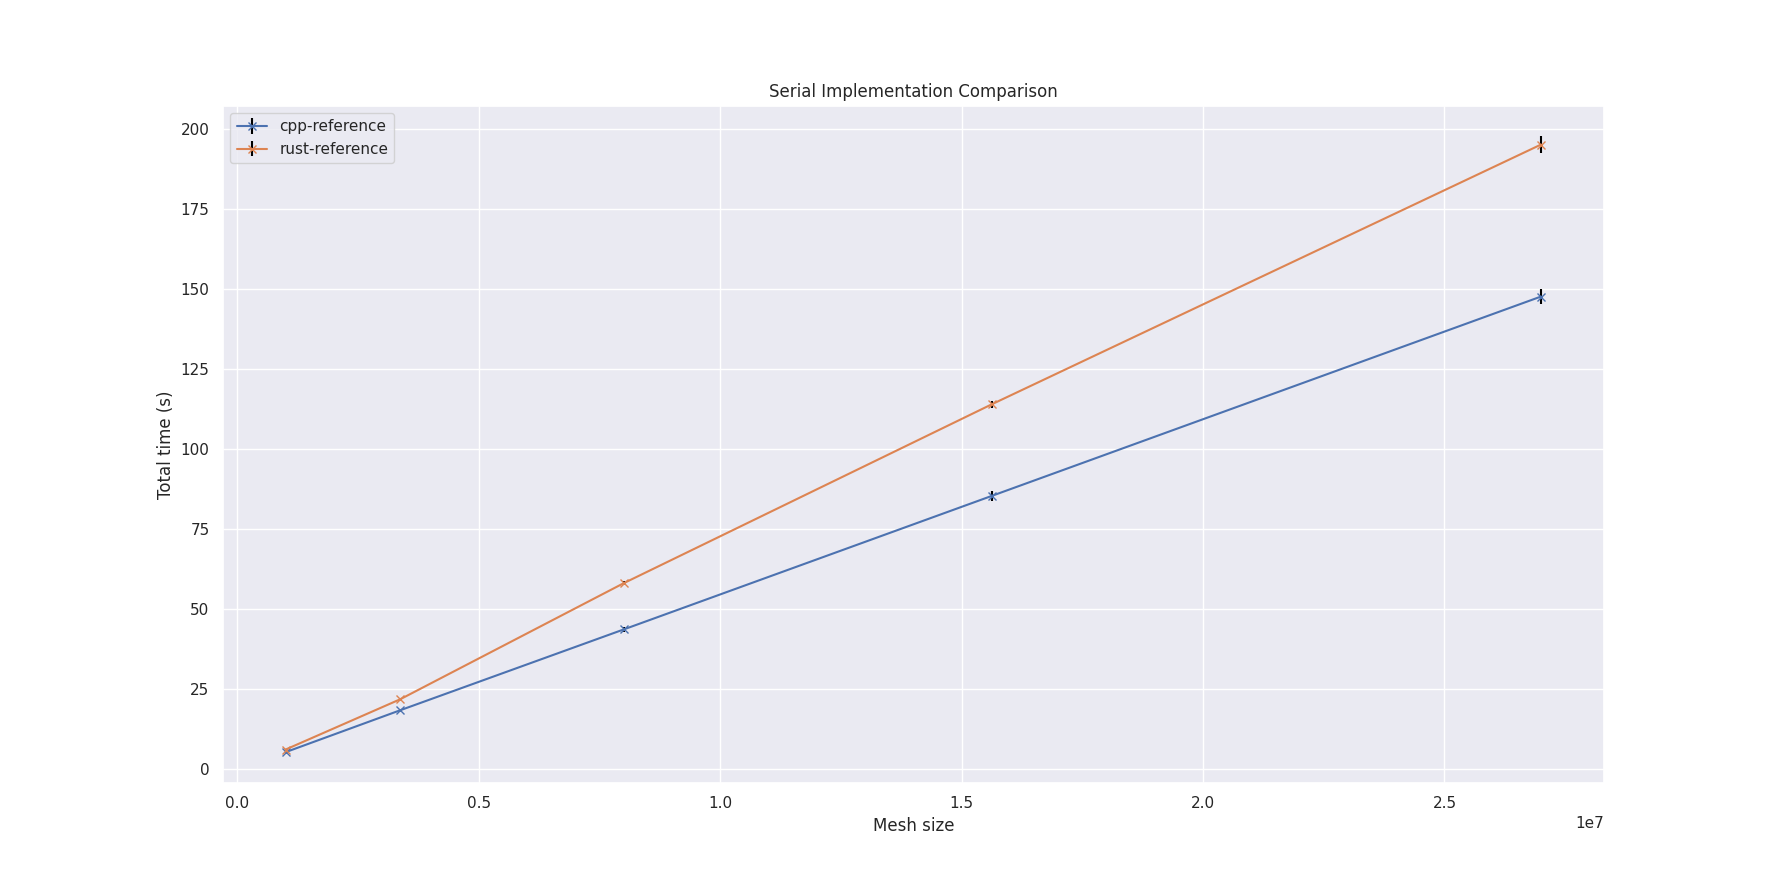
\includegraphics[width=\textwidth]{images/5_performance/parallelism/1_serial_line.png}
    \caption{A line plot comparing the total wall times for serial Rust and C++ implementations of HPCCG, on the Kudu batch compute system.}
    \label{fig:1_serial_line}
\end{figure}

\begin{figure}[H]
    \centering
    % This file was created with tikzplotlib v0.10.1.
\begin{tikzpicture}

\definecolor{darkorange25512714}{RGB}{255,127,14}
\definecolor{darkslategray38}{RGB}{38,38,38}
\definecolor{lightgray204}{RGB}{204,204,204}
\definecolor{steelblue31119180}{RGB}{31,119,180}

\begin{axis}[
axis line style={lightgray204},
height=0.45\textheight,
legend cell align={left},
legend style={fill opacity=0.8, draw opacity=1, text opacity=1, at={(0.91,0.5)}, anchor=east, draw=none},
tick align=outside,
tick pos=left,
title={Serial Implementation Relative Execution Times},
width=\textwidth,
x grid style={lightgray204},
xlabel=\textcolor{darkslategray38}{Mesh size},
xmajorgrids,
xmin=-300000, xmax=28300000,
xtick style={color=darkslategray38},
xtick={-5000000,0,5000000,10000000,15000000,20000000,25000000,30000000},
xticklabels={\ensuremath{-}0.5,0.0,0.5,1.0,1.5,2.0,2.5,3.0},
y grid style={lightgray204},
ylabel=\textcolor{darkslategray38}{Execution time relative to C++},
ymajorgrids,
ymin=0.981930448825138, ymax=1.3794605746721,
ytick style={color=darkslategray38}
]
\path [draw=black, semithick]
(axis cs:1000000,1)
--(axis cs:1000000,1);

\path [draw=black, semithick]
(axis cs:3375000,1)
--(axis cs:3375000,1);

\path [draw=black, semithick]
(axis cs:8000000,1)
--(axis cs:8000000,1);

\path [draw=black, semithick]
(axis cs:15625000,1)
--(axis cs:15625000,1);

\path [draw=black, semithick]
(axis cs:27000000,1)
--(axis cs:27000000,1);

\path [draw=black, semithick]
(axis cs:1000000,1.1347863488433)
--(axis cs:1000000,1.17350077973917);

\path [draw=black, semithick]
(axis cs:3375000,1.17279820962307)
--(axis cs:3375000,1.19987645999062);

\path [draw=black, semithick]
(axis cs:8000000,1.30733849198599)
--(axis cs:8000000,1.35448223973949);

\path [draw=black, semithick]
(axis cs:15625000,1.30895014587908)
--(axis cs:15625000,1.36139102349724);

\path [draw=black, semithick]
(axis cs:27000000,1.29392040608502)
--(axis cs:27000000,1.34917953583383);

\addplot [semithick, steelblue31119180, mark=x, mark size=3, mark options={solid}]
table {%
1000000 1
3375000 1
8000000 1
15625000 1
27000000 1
};
\addlegendentry{Baseline serial C++}
\addplot [semithick, darkorange25512714, mark=x, mark size=3, mark options={solid}]
table {%
1000000 1.15414357185364
3375000 1.18633735179901
8000000 1.33091032505035
15625000 1.33517062664032
27000000 1.32155001163483
};
\addlegendentry{Relative serial Rust}
\end{axis}

\end{tikzpicture}

    \vspace*{-0.5cm}
    % 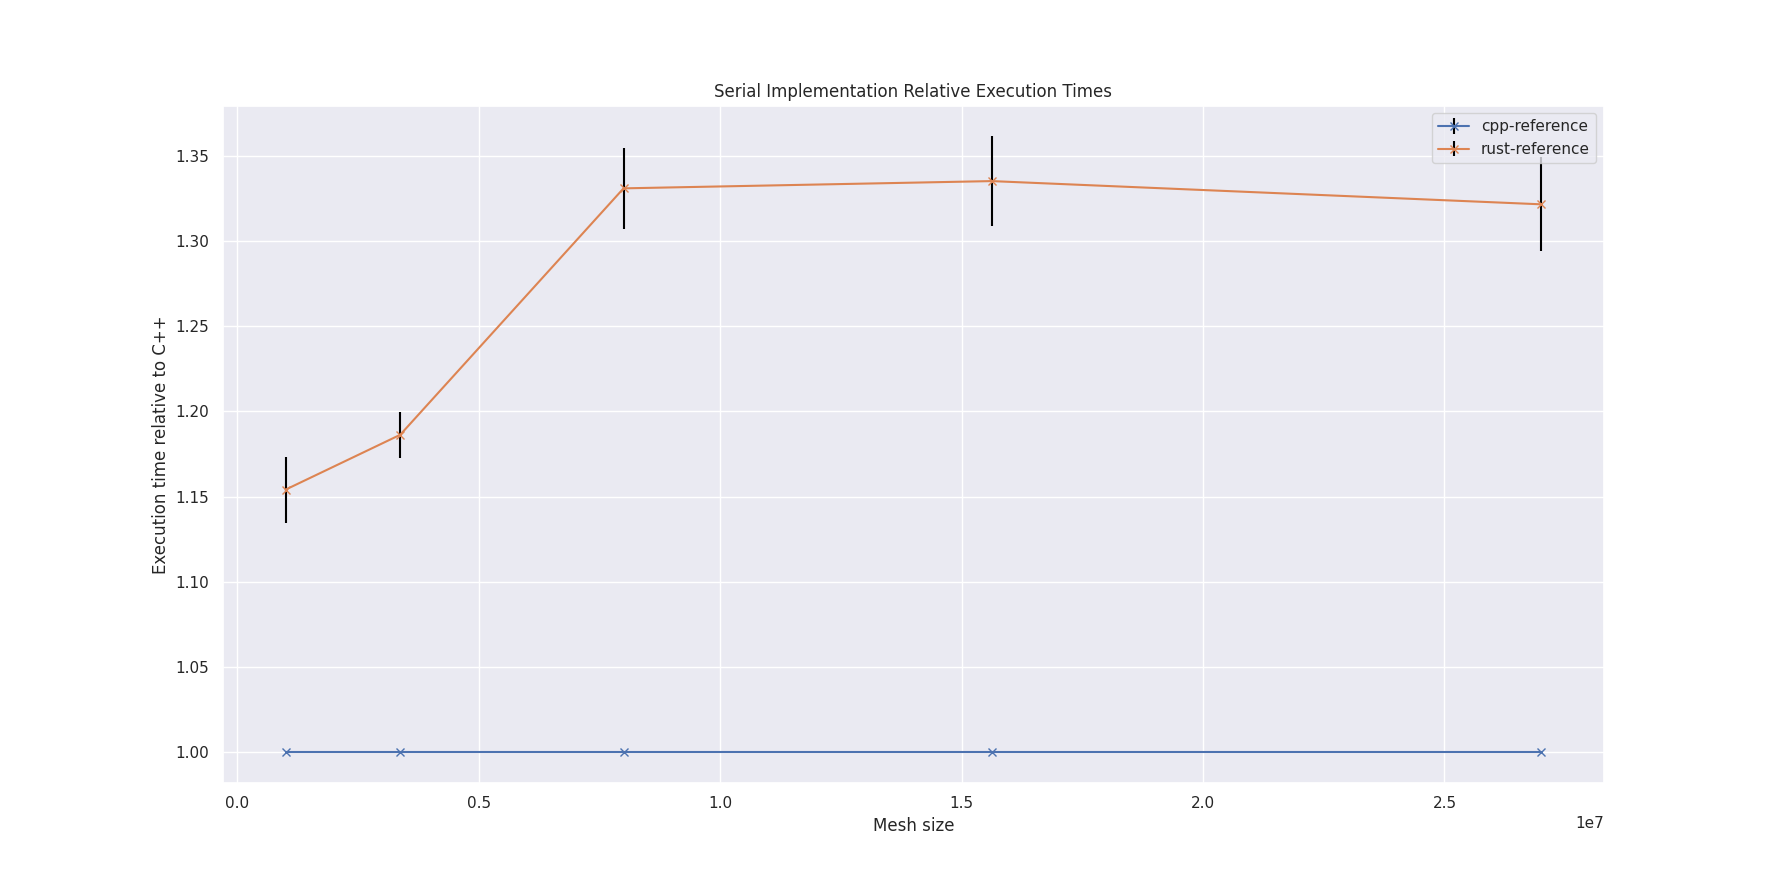
\includegraphics[width=\textwidth]{images/5_performance/parallelism/2_serial_line_relative.png}
    \caption{A line plot comparing the total wall times relative to the serial C++ implementation of HPCCG, on the Kudu batch compute system.}
    \label{fig:2_serial_line_relative}
\end{figure}

\begin{figure}[H]
    \centering
    % This file was created with tikzplotlib v0.10.1.
\begin{tikzpicture}

\definecolor{darkorange25512714}{RGB}{255,127,14}
\definecolor{darkslategray38}{RGB}{38,38,38}
\definecolor{lightgray204}{RGB}{204,204,204}
\definecolor{steelblue31119180}{RGB}{31,119,180}

\begin{axis}[
axis line style={lightgray204},
height=0.375\textheight,
legend cell align={left},
legend style={
  fill opacity=0.8,
  draw opacity=1,
  text opacity=1,
  at={(0.03,0.97)},
  anchor=north west,
  % draw=none
},
tick align=outside,
tick pos=left,
title={Serial Implementation Comparison},
width=\textwidth,
x grid style={lightgray204},
xlabel=\textcolor{darkslategray38}{Mesh size},
xmajorgrids,
xmin=-300000, xmax=28300000,
xtick style={color=darkslategray38},
xtick={-5000000,0,5000000,10000000,15000000,20000000,25000000,30000000},
xticklabels={\ensuremath{-}0.5,0.0,0.5,1.0,1.5,2.0,2.5,3.0},
y grid style={lightgray204},
ylabel=\textcolor{darkslategray38}{Total time (s)},
ymajorgrids,
ymin=-4.88467607640496, ymax=216.204185900316,
ytick style={color=darkslategray38}
]
\path [draw=black, semithick]
(axis cs:1000000,5.16481764980962)
--(axis cs:1000000,5.63830735019038);

\path [draw=black, semithick]
(axis cs:3375000,19.113269268153)
--(axis cs:3375000,19.198180731847);

\path [draw=black, semithick]
(axis cs:8000000,45.0572061385652)
--(axis cs:8000000,46.2580438614348);

\path [draw=black, semithick]
(axis cs:15625000,84.9558151201549)
--(axis cs:15625000,88.3661348798451);

\path [draw=black, semithick]
(axis cs:27000000,144.202737917063)
--(axis cs:27000000,154.023762082937);

\path [draw=black, semithick]
(axis cs:1000000,6.85489901375067)
--(axis cs:1000000,7.18950098624933);

\path [draw=black, semithick]
(axis cs:3375000,22.1573131184878)
--(axis cs:3375000,23.3257368815122);

\path [draw=black, semithick]
(axis cs:8000000,60.0949440654008)
--(axis cs:8000000,61.7840559345992);

\path [draw=black, semithick]
(axis cs:15625000,118.342476046812)
--(axis cs:15625000,120.701023953188);

\path [draw=black, semithick]
(axis cs:27000000,196.585857825899)
--(axis cs:27000000,206.154692174101);

\addplot [semithick, steelblue31119180, mark=x, mark size=3, mark options={solid}]
table {%
1000000 5.40156269073486
3375000 19.155725479126
8000000 45.6576232910156
15625000 86.6609725952148
27000000 149.113250732422
};
\addlegendentry{Serial C++}
\addplot [semithick, darkorange25512714, mark=triangle, mark size=3, mark options={solid}]
table {%
1000000 7.02220010757446
3375000 22.7415256500244
8000000 60.9394989013672
15625000 119.521751403809
27000000 201.370269775391
};
\addlegendentry{Serial Rust}
\end{axis}

\end{tikzpicture}

    \vspace*{-0.5cm}
    % 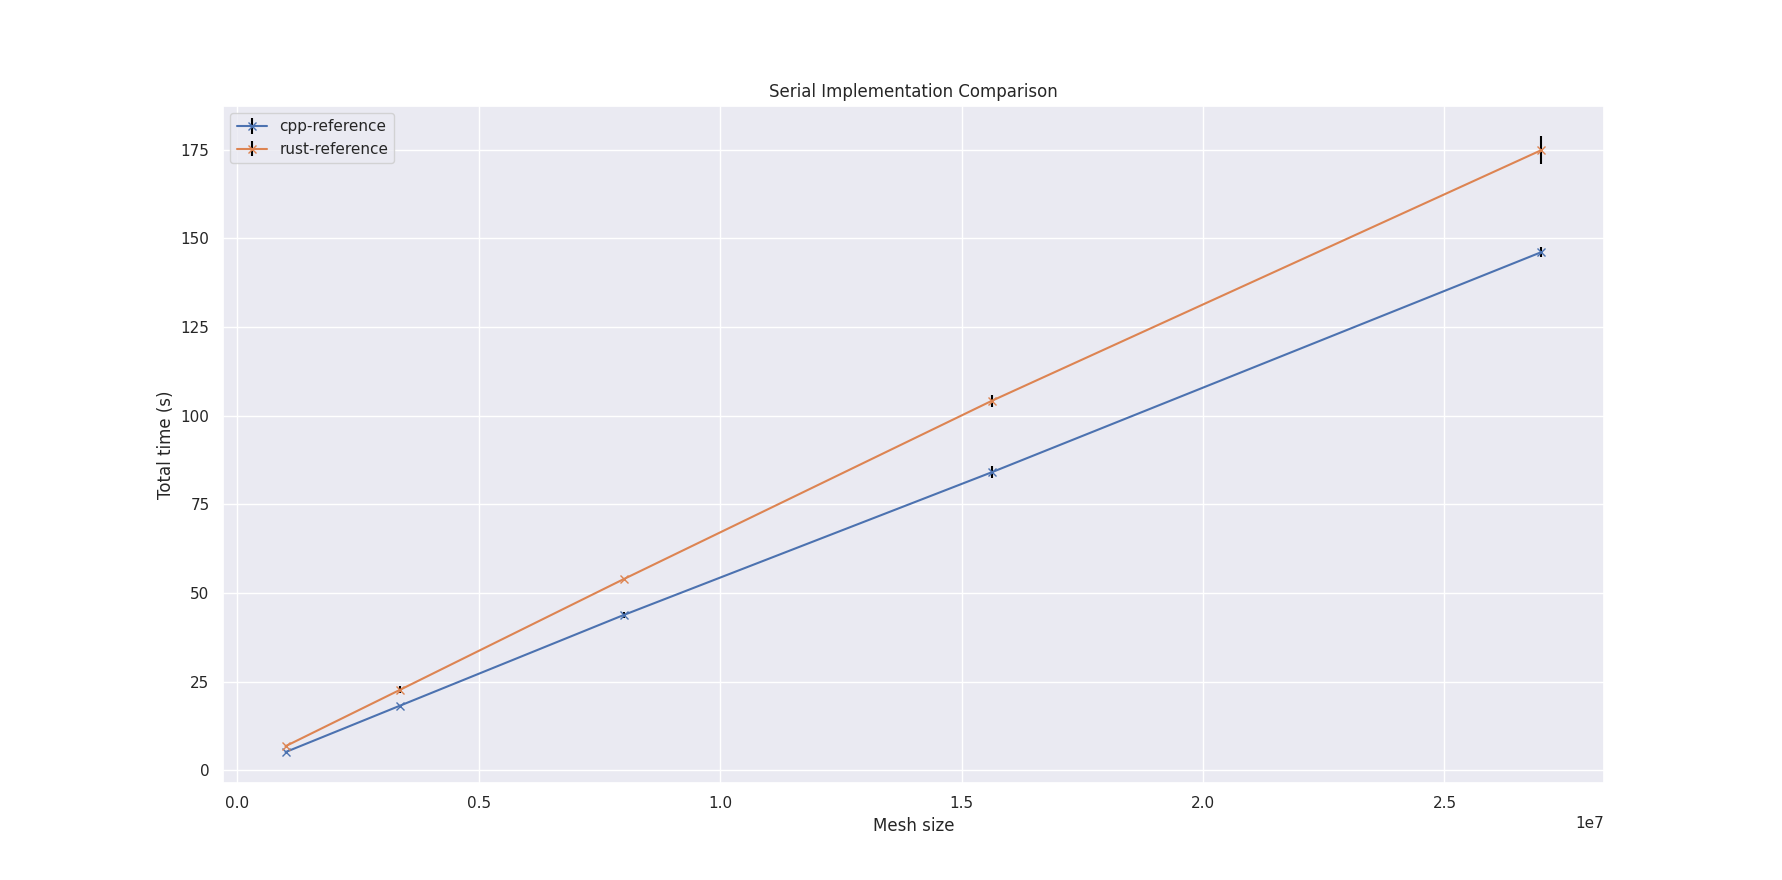
\includegraphics[width=\textwidth]{images/5_performance/parallelism/1_serial_line_avon.png}
    \caption{A line plot comparing the total wall times across all computational kernels for serial Rust and C++ implementations of HPCCG, on the Avon batch compute system.}
    \label{fig:1_serial_line_avon}
\end{figure}

\begin{figure}[H]
    \centering
    % This file was created with tikzplotlib v0.10.1.
\begin{tikzpicture}

\definecolor{darkorange25512714}{RGB}{255,127,14}
\definecolor{darkslategray38}{RGB}{38,38,38}
\definecolor{lightgray204}{RGB}{204,204,204}
\definecolor{steelblue31119180}{RGB}{31,119,180}

\begin{axis}[
axis line style={lightgray204},
height=0.45\textheight,
legend cell align={left},
legend style={
  fill opacity=0.8,
  draw opacity=1,
  text opacity=1,
  at={(0.03,0.97)},
  anchor=north west,
  draw=none
},
tick align=outside,
tick pos=left,
title={Serial Implementation Relative Execution Times},
width=\textwidth,
x grid style={lightgray204},
xlabel=\textcolor{darkslategray38}{Mesh size},
xmajorgrids,
xmin=-300000, xmax=28300000,
xtick style={color=darkslategray38},
xtick={-5000000,0,5000000,10000000,15000000,20000000,25000000,30000000},
xticklabels={\ensuremath{-}0.5,0.0,0.5,1.0,1.5,2.0,2.5,3.0},
y grid style={lightgray204},
ylabel=\textcolor{darkslategray38}{Execution time relative to C++},
ymajorgrids,
ymin=0.979522720404777, ymax=1.43002287149969,
ytick style={color=darkslategray38}
]
\path [draw=black, semithick]
(axis cs:1000000,1)
--(axis cs:1000000,1);

\path [draw=black, semithick]
(axis cs:3375000,1)
--(axis cs:3375000,1);

\path [draw=black, semithick]
(axis cs:8000000,1)
--(axis cs:8000000,1);

\path [draw=black, semithick]
(axis cs:15625000,1)
--(axis cs:15625000,1);

\path [draw=black, semithick]
(axis cs:27000000,1)
--(axis cs:27000000,1);

\path [draw=black, semithick]
(axis cs:1000000,1.23517820533607)
--(axis cs:1000000,1.36488427658467);

\path [draw=black, semithick]
(axis cs:3375000,1.15658075460817)
--(axis cs:3375000,1.21780340469668);

\path [draw=black, semithick]
(axis cs:8000000,1.30920619293907)
--(axis cs:8000000,1.36020554277868);

\path [draw=black, semithick]
(axis cs:15625000,1.34882978986339)
--(axis cs:15625000,1.40954559190447);

\path [draw=black, semithick]
(axis cs:27000000,1.29561320828562)
--(axis cs:27000000,1.40529063493421);

\addplot [semithick, steelblue31119180, mark=x, mark size=3, mark options={solid}]
table {%
1000000 1
3375000 1
8000000 1
15625000 1
27000000 1
};
\addlegendentry{Baseline serial C++}
\addplot [semithick, darkorange25512714, mark=x, mark size=3, mark options={solid}]
table {%
1000000 1.30003118515015
3375000 1.18719208240509
8000000 1.33470582962036
15625000 1.37918770313263
27000000 1.35045194625854
};
\addlegendentry{Relative serial Rust}
\end{axis}

\end{tikzpicture}

    \vspace*{-0.5cm}
    % 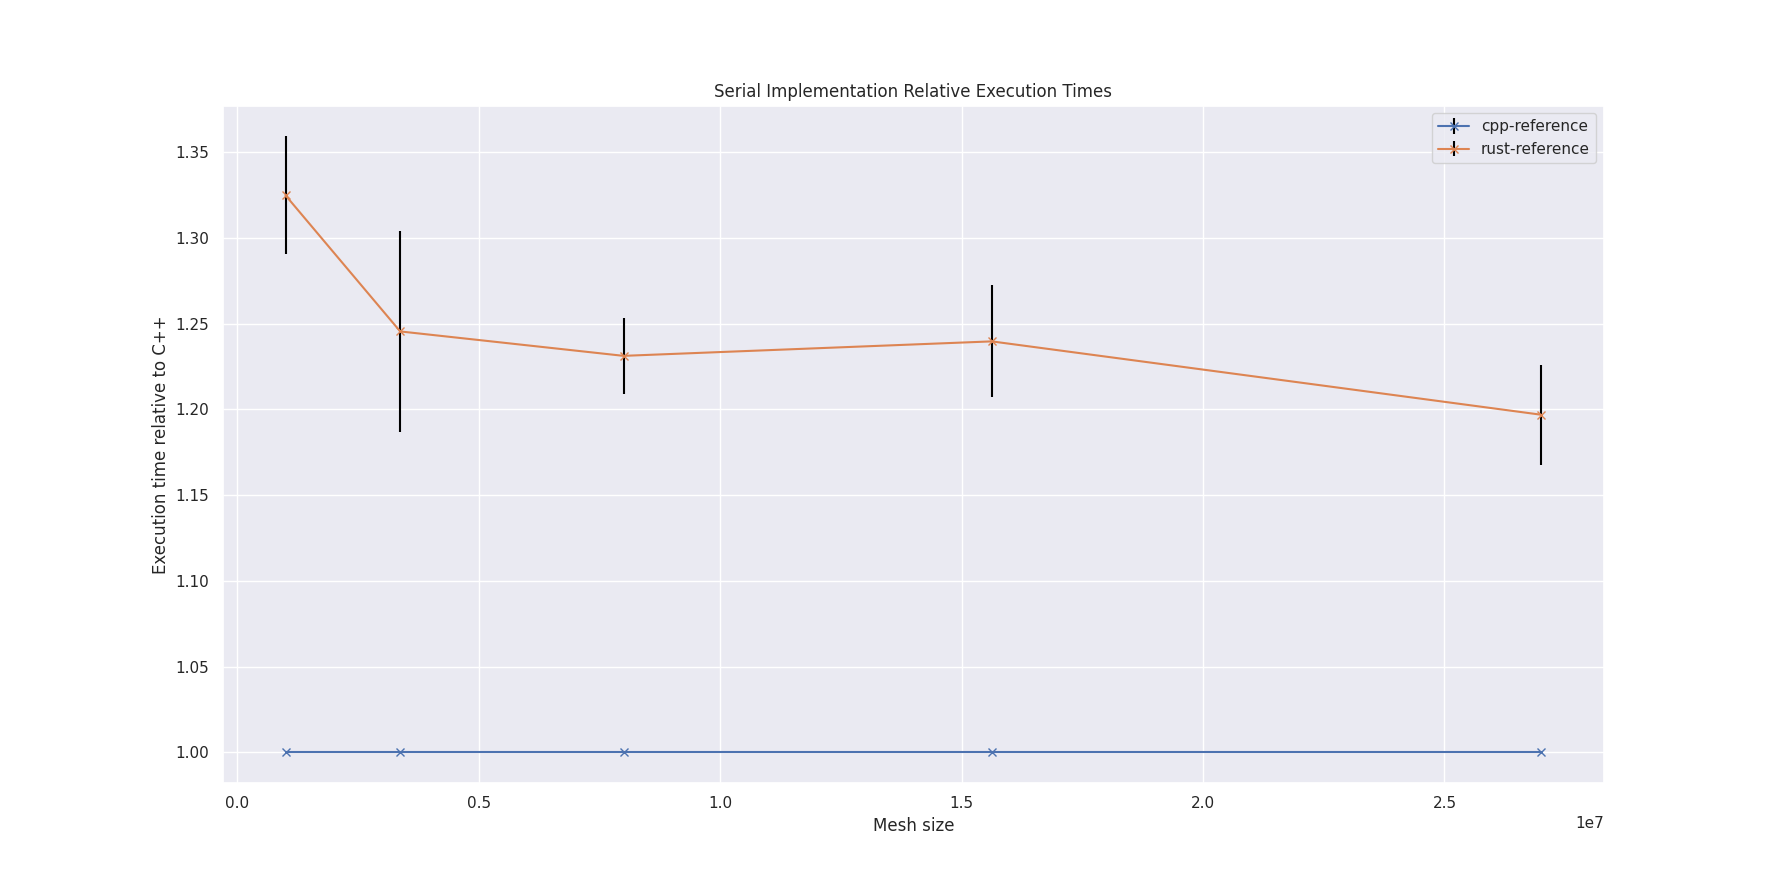
\includegraphics[width=\textwidth]{images/5_performance/parallelism/2_serial_line_relative_avon.png}
    \caption{A line plot comparing the total wall times relative to the serial C++ implementation of HPCCG, on the Avon batch compute system.}
    \label{fig:2_serial_line_relative_avon}
\end{figure}


In summary, Rust is competitively performant for serial workloads, but trails C++ in performance, converging to around a $1.33 \pm 0.02 \times$ slow-down on Kudu and $1.21 \pm 0.03 \times$ slow down on Avon for large mesh sizes.

Finally, we can see that tests run on Avon and Kudu have very similar performance characteristics. This is encouraging, since it suggests that Rust is portable across compute cluster topologies, albeit having only tested on Intel CPUs. As a result of this, future plots will shown only the results of runs on Kudu for brevity, unless otherwise stated. The plots for runs on Avon can be generated using the HPC MultiBench tool from the data provided in the \texttt{hpccg-rs-avon-results} repository, as discussed in section \ref{sssec:parallelism-approaches-reproducibility}.

\subsection{Multi-threading}
\label{ssec:multi-threaded}

Having evaluated serial execution, the next parallelisation strategy to consider is shared memory parallelism through multi-threading. This is typically used for parallelism within a single machine, but it can also be used in combination with MPI for nodes in a cluster.
% As it is such a ubiquitous mechanism of parallelisation, along with frameworks such as OpenMP and Rayon which provide convenient abstractions over it, multi-threading is a critical aspect of writing performant code in High-Performance Computing.

To assess multithreaded performance, we ran the C++ and Rust executables over both a range of mesh sizes, from $100 \times 100 \times 100$ to $400 \times 400 \times 400$, incrementing each axis size by $100$ each time, and a range of thread counts: $1$, $8$, and $32$. In addition to the experimental methodology discussed in section \ref{ssec:experimental-methodology}, all parallel runs were conducted on a single node in the compute cluster, with a single task per node, and 32 threads allocated per task, along with exclusive use of that node to reduce machine noise from other processes.
% As discussed in the previous section, only runs from the Kudu batch compute system will be shown for brevity, unless the results on Avon notably differ.
The results of these experiments are shown in Figures \ref{fig:5_parallel_line_all} and \ref{fig:7_parallel_line_relative}.

\begin{figure}[H]
    \centering
    % This file was created with tikzplotlib v0.10.1.
\begin{tikzpicture}

\definecolor{crimson2143940}{RGB}{214,39,40}
\definecolor{darkorange25512714}{RGB}{255,127,14}
\definecolor{darkslategray38}{RGB}{38,38,38}
\definecolor{forestgreen4416044}{RGB}{44,160,44}
\definecolor{lightgray204}{RGB}{204,204,204}
\definecolor{mediumpurple148103189}{RGB}{148,103,189}
\definecolor{sienna1408675}{RGB}{140,86,75}
\definecolor{steelblue31119180}{RGB}{31,119,180}

\begin{axis}[
axis line style={lightgray204},
height=0.45\textheight,
legend cell align={left},
legend style={
  fill opacity=0.8,
  draw opacity=1,
  text opacity=1,
  at={(0.03,0.97)},
  anchor=north west,
  % draw=none
},
tick align=outside,
tick pos=left,
title={Multi-Threaded Implementation Comparison},
width=\textwidth,
x grid style={lightgray204},
xlabel=\textcolor{darkslategray38}{Mesh size},
xmajorgrids,
xmin=-2150000, xmax=67150000,
xtick style={color=darkslategray38},
xtick={-10000000,0,10000000,20000000,30000000,40000000,50000000,60000000,70000000},
xticklabels={\ensuremath{-}1,0,1,2,3,4,5,6,7},
y grid style={lightgray204},
ylabel=\textcolor{darkslategray38}{Total time (s)},
ymajorgrids,
ymin=-25.7913154590251, ymax=575.329051768724,
ytick style={color=darkslategray38}
]
\path [draw=black, semithick]
(axis cs:1000000,5.34438827454193)
--(axis cs:1000000,5.42485172545807);

\path [draw=black, semithick]
(axis cs:8000000,43.7885345691461)
--(axis cs:8000000,44.5500654308539);

\path [draw=black, semithick]
(axis cs:27000000,148.452354955297)
--(axis cs:27000000,150.368145044703);

\path [draw=black, semithick]
(axis cs:64000000,348.323499523336)
--(axis cs:64000000,360.386500476664);

\path [draw=black, semithick]
(axis cs:1000000,1.61017148732022)
--(axis cs:1000000,1.74248851267978);

\path [draw=black, semithick]
(axis cs:8000000,10.0397988826484)
--(axis cs:8000000,11.9477361173516);

\path [draw=black, semithick]
(axis cs:27000000,27.8186839726246)
--(axis cs:27000000,30.4796160273754);

\path [draw=black, semithick]
(axis cs:64000000,63.0155340032716)
--(axis cs:64000000,65.5569159967284);

\path [draw=black, semithick]
(axis cs:1000000,2.21986248923652)
--(axis cs:1000000,2.41283751076348);

\path [draw=black, semithick]
(axis cs:8000000,9.33409289646281)
--(axis cs:8000000,10.1720021035372);

\path [draw=black, semithick]
(axis cs:27000000,22.7588093641245)
--(axis cs:27000000,24.2544906358755);

\path [draw=black, semithick]
(axis cs:64000000,52.406768330518)
--(axis cs:64000000,52.568581669482);

\path [draw=black, semithick]
(axis cs:1000000,6.25873918999268)
--(axis cs:1000000,6.82466081000732);

\path [draw=black, semithick]
(axis cs:8000000,63.8942873740022)
--(axis cs:8000000,65.7118626259978);

\path [draw=black, semithick]
(axis cs:27000000,204.746427561689)
--(axis cs:27000000,230.781572438311);

\path [draw=black, semithick]
(axis cs:64000000,499.593601287083)
--(axis cs:64000000,548.005398712917);

\path [draw=black, semithick]
(axis cs:1000000,1.65376688002974)
--(axis cs:1000000,1.85328311997026);

\path [draw=black, semithick]
(axis cs:8000000,14.3098625303521)
--(axis cs:8000000,14.8229374696479);

\path [draw=black, semithick]
(axis cs:27000000,46.0131259435759)
--(axis cs:27000000,46.5430240564241);

\path [draw=black, semithick]
(axis cs:64000000,99.2363635122588)
--(axis cs:64000000,103.493086487741);

\path [draw=black, semithick]
(axis cs:1000000,1.53233759678168)
--(axis cs:1000000,1.54256240321832);

\path [draw=black, semithick]
(axis cs:8000000,11.7334601576525)
--(axis cs:8000000,11.8162898423475);

\path [draw=black, semithick]
(axis cs:27000000,36.4014166698829)
--(axis cs:27000000,36.4877833301171);

\path [draw=black, semithick]
(axis cs:64000000,84.8465319256481)
--(axis cs:64000000,85.3538180743519);

\addplot [semithick, steelblue31119180, mark=x, mark size=3, mark options={solid}]
table {%
1000000 5.38462018966675
8000000 44.1693000793457
27000000 149.410247802734
64000000 354.355010986328
};
\addlegendentry{C++ with 1 OpenMP thread}
\addplot [semithick, darkorange25512714, mark=triangle, mark size=3, mark options={solid}]
table {%
1000000 1.6763299703598
8000000 10.9937677383423
27000000 29.1491508483887
64000000 64.2862243652344
};
\addlegendentry{C++ with 8 OpenMP threads}
\addplot [semithick, forestgreen4416044, mark=star, mark size=3, mark options={solid}]
table {%
1000000 2.31634998321533
8000000 9.75304794311523
27000000 23.5066509246826
64000000 52.4876747131348
};
\addlegendentry{C++ with 32 OpenMP threads}
\addplot [semithick, crimson2143940, mark=diamond, mark size=3, mark options={solid}]
table {%
1000000 6.54169988632202
8000000 64.8030776977539
27000000 217.764007568359
64000000 523.799499511719
};
\addlegendentry{Rust with 1 Rayon thread}
\addplot [semithick, mediumpurple148103189, mark=square, mark size=3, mark options={solid}]
table {%
1000000 1.75352501869202
8000000 14.5663995742798
27000000 46.278076171875
64000000 101.364723205566
};
\addlegendentry{Rust with 8 Rayon threads}
\addplot [semithick, sienna1408675, mark=o, mark size=3, mark options={solid}]
table {%
1000000 1.53744995594025
8000000 11.7748746871948
27000000 36.4445991516113
64000000 85.1001739501953
};
\addlegendentry{Rust with 32 Rayon threads}
\end{axis}

\end{tikzpicture}

    \vspace*{-0.5cm}
    % 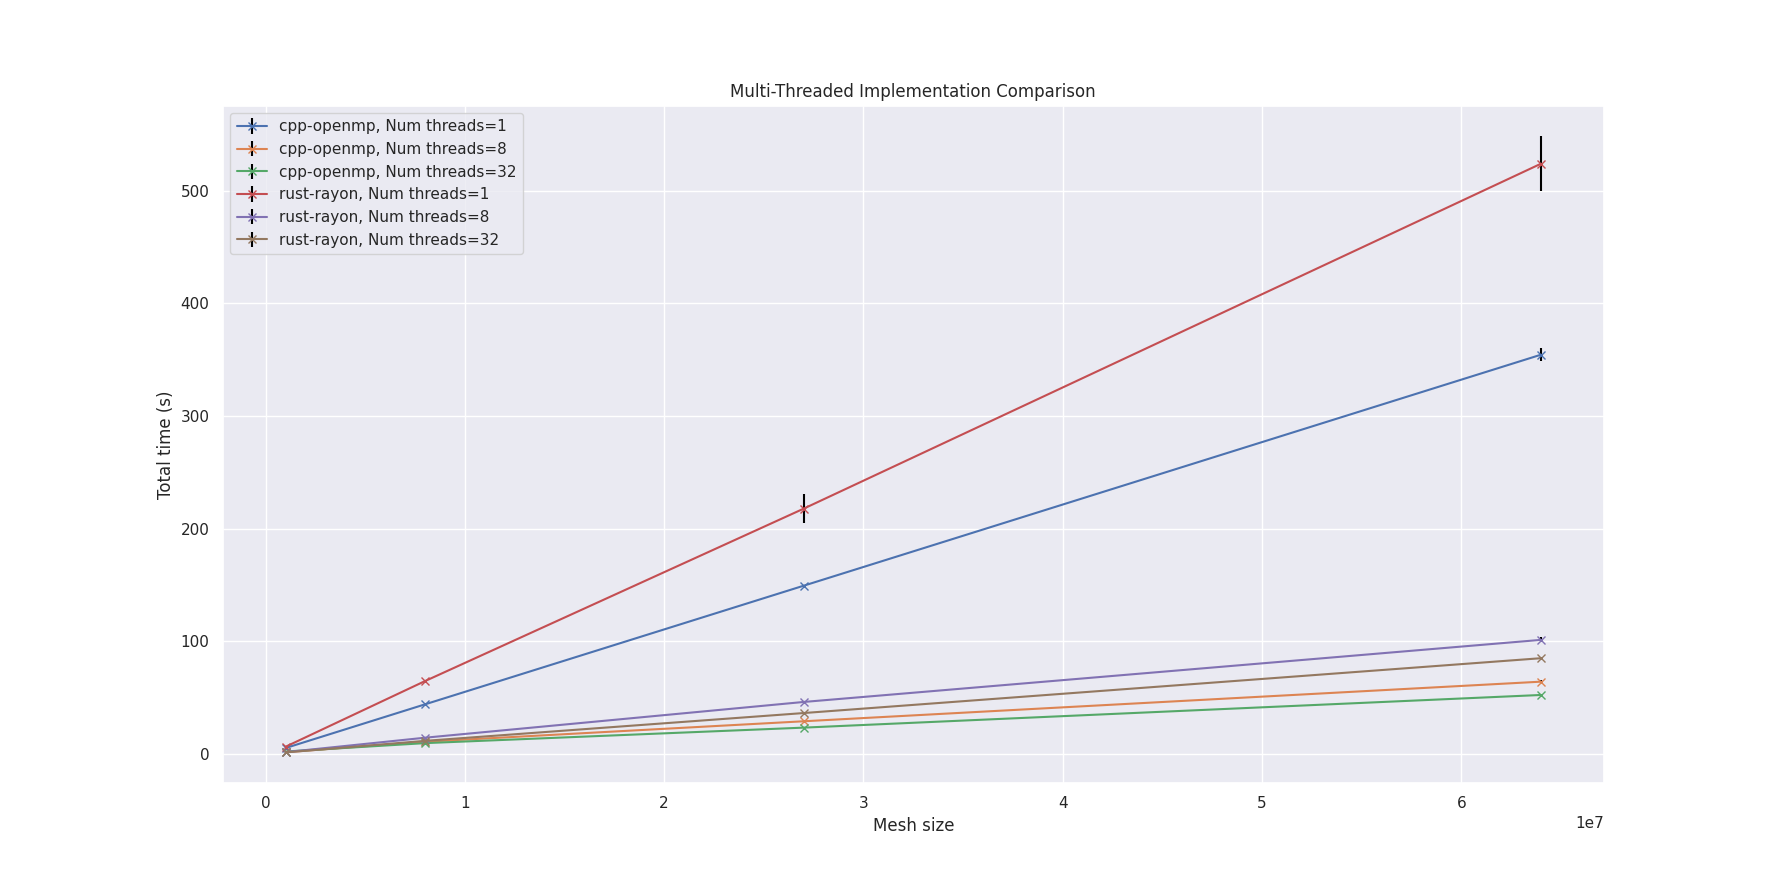
\includegraphics[width=\textwidth]{images/5_performance/parallelism/5_parallel_line_all.png}
    \caption{A line plot comparing the total wall times across all computational kernels for multithreaded Rust and C++ implementations of HPCCG.}
    \label{fig:5_parallel_line_all}
\end{figure}

% TODO: Error bars are unreadable here
\begin{figure}[H]
    \centering
    % This file was created with tikzplotlib v0.10.1.
\begin{tikzpicture}

\definecolor{crimson2143940}{RGB}{214,39,40}
\definecolor{darkorange25512714}{RGB}{255,127,14}
\definecolor{darkslategray38}{RGB}{38,38,38}
\definecolor{forestgreen4416044}{RGB}{44,160,44}
\definecolor{lightgray204}{RGB}{204,204,204}
\definecolor{mediumpurple148103189}{RGB}{148,103,189}
\definecolor{sienna1408675}{RGB}{140,86,75}
\definecolor{steelblue31119180}{RGB}{31,119,180}

\begin{axis}[
axis line style={lightgray204},
height=0.45\textheight,
legend cell align={left},
legend style={fill opacity=0.8, draw opacity=1, text opacity=1, anchor=south east, draw=none},
tick align=outside,
tick pos=left,
title={Multi-Threaded Implementation Relative Execution Times},
width=\textwidth,
x grid style={lightgray204},
xlabel=\textcolor{darkslategray38}{Mesh size},
xmajorgrids,
xmin=-2150000, xmax=67150000,
xtick style={color=darkslategray38},
xtick={-10000000,0,10000000,20000000,30000000,40000000,50000000,60000000,70000000},
xticklabels={\ensuremath{-}1,0,1,2,3,4,5,6,7},
y grid style={lightgray204},
ylabel=\textcolor{darkslategray38}{Execution time relative to C++},
ymajorgrids,
ymin=0.584769215693879, ymax=1.71189604011066,
ytick style={color=darkslategray38}
]
\path [draw=black, semithick]
(axis cs:1000000,1)
--(axis cs:1000000,1);

\path [draw=black, semithick]
(axis cs:8000000,1)
--(axis cs:8000000,1);

\path [draw=black, semithick]
(axis cs:27000000,1)
--(axis cs:27000000,1);

\path [draw=black, semithick]
(axis cs:64000000,1)
--(axis cs:64000000,1);

\path [draw=black, semithick]
(axis cs:1000000,1.16155807824418)
--(axis cs:1000000,1.26821412480822);

\path [draw=black, semithick]
(axis cs:8000000,1.44300036800877)
--(axis cs:8000000,1.49130354896523);

\path [draw=black, semithick]
(axis cs:27000000,1.36986435112552)
--(axis cs:27000000,1.54511638145474);

\path [draw=black, semithick]
(axis cs:64000000,1.40538127443367)
--(axis cs:64000000,1.55097322881872);

\path [draw=black, semithick]
(axis cs:1000000,0.973622351332752)
--(axis cs:1000000,1.11847765284304);

\path [draw=black, semithick]
(axis cs:8000000,1.20765247313455)
--(axis cs:8000000,1.44228532116572);

\path [draw=black, semithick]
(axis cs:27000000,1.5145976824943)
--(axis cs:27000000,1.66066300263717);

\path [draw=black, semithick]
(axis cs:64000000,1.53130258066264)
--(axis cs:64000000,1.62224158840313);

\path [draw=black, semithick]
(axis cs:1000000,0.636002253167369)
--(axis cs:1000000,0.691474164472452);

\path [draw=black, semithick]
(axis cs:8000000,1.15526737082365)
--(axis cs:8000000,1.25933688492308);

\path [draw=black, semithick]
(axis cs:27000000,1.50103683366645)
--(axis cs:27000000,1.59975379366666);

\path [draw=black, semithick]
(axis cs:64000000,1.61589590433844)
--(axis cs:64000000,1.62677678024894);

\addplot [semithick, steelblue31119180, mark=x, mark size=3, mark options={solid}]
table {%
1000000 1
8000000 1
27000000 1
64000000 1
};
\addlegendentry{C++ with 1 OpenMP thread}
\addplot [semithick, darkorange25512714, mark=x, mark size=3, mark options={solid}]
table {%
1000000 1
8000000 1
27000000 1
64000000 1
};
\addlegendentry{C++ with 8 OpenMP threads}
\addplot [semithick, forestgreen4416044, mark=x, mark size=3, mark options={solid}]
table {%
1000000 1
8000000 1
27000000 1
64000000 1
};
\addlegendentry{C++ with 32 OpenMP threads}
\addplot [semithick, crimson2143940, mark=x, mark size=3, mark options={solid}]
table {%
1000000 1.21488606929779
8000000 1.46715199947357
27000000 1.45749032497406
64000000 1.47817730903625
};
\addlegendentry{Rust with 1 Rayon thread}
\addplot [semithick, mediumpurple148103189, mark=x, mark size=3, mark options={solid}]
table {%
1000000 1.04604995250702
8000000 1.32496893405914
27000000 1.58763039112091
64000000 1.57677209377289
};
\addlegendentry{Rust with 8 Rayon threads}
\addplot [semithick, sienna1408675, mark=x, mark size=3, mark options={solid}]
table {%
1000000 0.663738250732422
8000000 1.20730209350586
27000000 1.55039536952972
64000000 1.62133634090424
};
\addlegendentry{Rust with 32 Rayon threads}
\end{axis}

\end{tikzpicture}

    \vspace*{-0.5cm}
    % 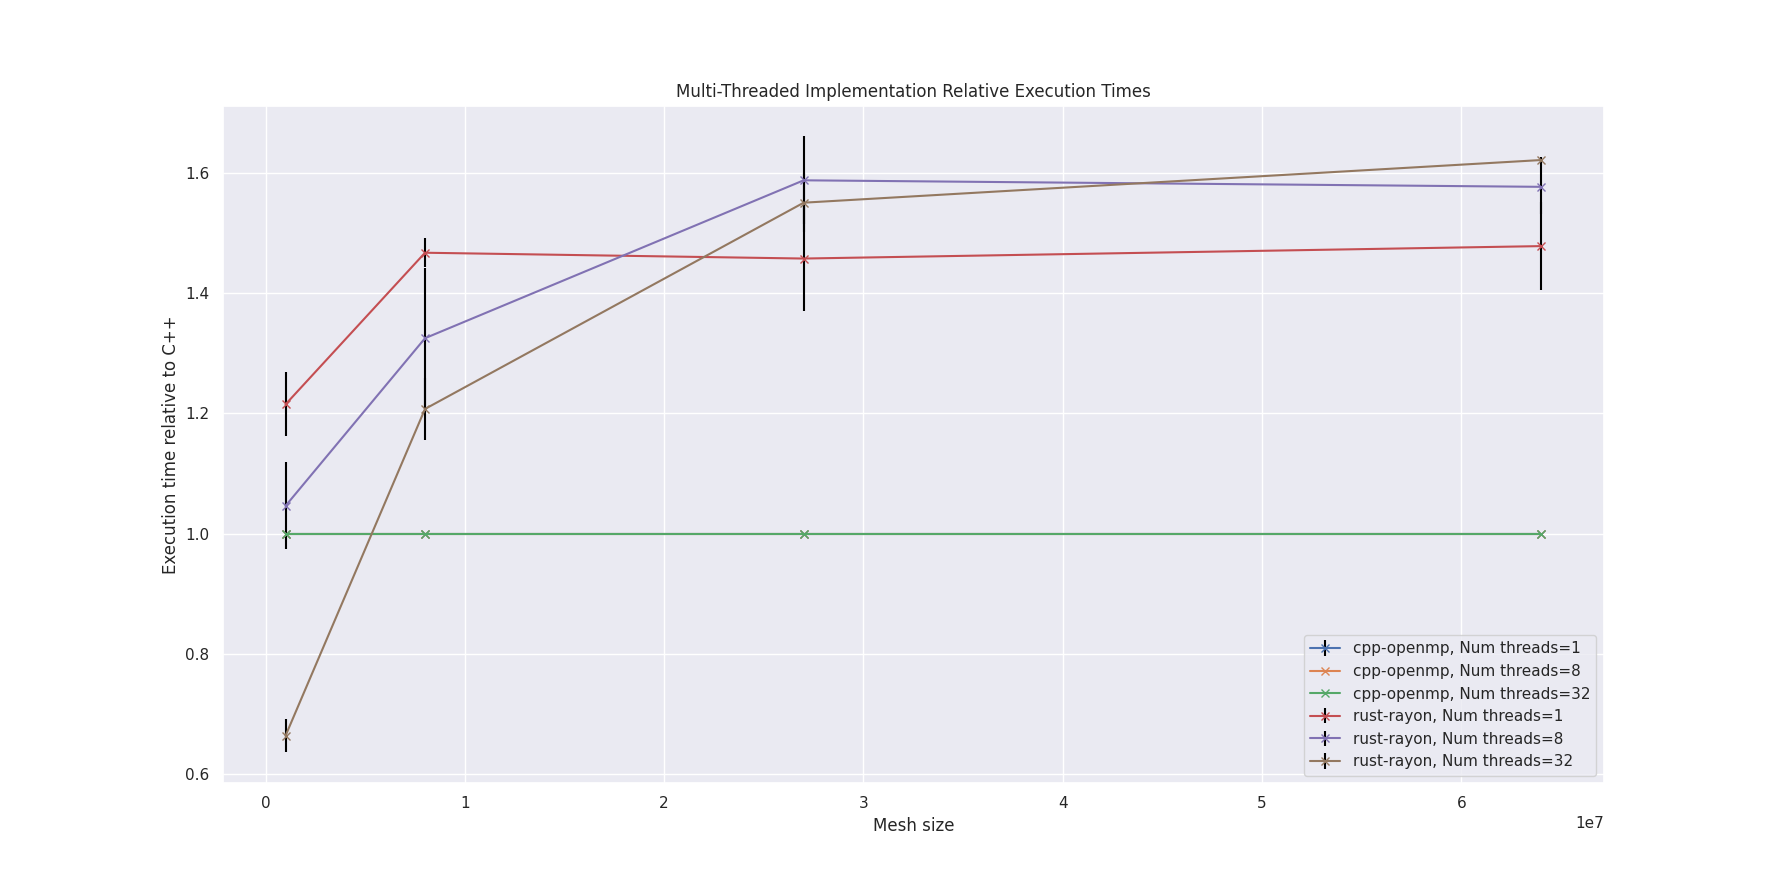
\includegraphics[width=\textwidth]{images/5_performance/parallelism/7_parallel_line_relative.png}
    \caption{A line plot comparing the total wall times relative to the multithreaded C++ implementation of HPCCG.}
    \label{fig:7_parallel_line_relative}
\end{figure}

% TODO: Add note about high error bars due to machine noise, amplified by inverse operation

From Figure \ref{fig:7_parallel_line_relative} which shows execution time relative to C++, we can see that for small meshes Rust with Rayon outperforms C++ with OpenMP increasingly with higher thread counts. For $100 \times 100 \times 100$ meshes with 32 threads, Rust takes $0.66 \pm 0.08 \times$ less runtime. This is likely because Rayon uses a work-stealing thread scheduling methodology, which means it avoids the overhead of allocating many threads for tasks too small to fully leverage them.

However, for the largest workload of $400 \times 400 \times 400$ rusts begins to significantly trail C++, with 32 threads being $1.621 \pm 0.005 \times$ slower. This slower runtime appears to converge for very large mesh sizes, for example with 8 threads, meshes with edge lengths of $300$ and $400$ overlap uncertainty intervals at $1.49 \pm 0.12$ and $1.51 \pm 0.11$ respectively. This convergence appears to occur later for higher thread counts, but further experimentation on a more capable machine would be required to confirm this.

In summary, Rust remains performant in multi-threading workloads, but trails C++ in performance with around a $1.5 \pm 0.1\times$ slow-down for large, highly parallel workloads. The results from runs on Avon match those from those shown above on Kudu, with the slowdown across threads similarly converging at around $1.5 \pm 0.25$.

\subsection{MPI}
\label{ssec:mpi}

Shared memory parallelism is a very powerful technique for enhancing program performance. However, its efficacy is upper bounded as its use is constrained to single machines with shared memory architectures. In order to scale beyond this, distributed memory parallelism must be leveraged. This is required for many High-Performance Computing applications, as the largest supercomputers are all composed of clusters of many machines \cite{HomeTOP500}.
% As discussed in the translation section \ref{}, Rust provides MPI bindings which facilitate this.

For the original MPI implementation, the largest mesh size that can be computed without error is constrained by the constant value \mintinline{c++}{const int max_external = 100000;}, which places an upper bound on the number of cells which can be transmitted between MPI ranks. As a result of this, the largest mesh size computable with two MPI ranks is limited to around $250 \times 250 \times 250$. In order to exercise the MPI implementation across more ranks and larger mesh sizes, the original HPCCG codebase was modified to set \mintinline{c++}{max_external} to the largest value encodable by a four byte integer, $2147483647$. This allowed very large experiments on meshes up to $800 \times 800 \times 800$ across 5 MPI ranks.

To assess Rust's performance using MPI for message passing, we ran the C++ and Rust executables over both a range of mesh sizes, from $25 \times 25 \times 25$ to $250 \times 250 \times 250$, incrementing each axis size first by $25$, then by $50$ each time. Two nodes and two MPI tasks per node were used in addition to the experimental methodology discussed in section \ref{ssec:experimental-methodology}. The results of these experiments are shown in Figures \ref{fig:9_mpi_line} and \ref{fig:10_mpi_line_relative}.


\begin{figure}[H]
    \centering
    % This file was created with tikzplotlib v0.10.1.
\begin{tikzpicture}

\definecolor{darkorange25512714}{RGB}{255,127,14}
\definecolor{darkslategray38}{RGB}{38,38,38}
\definecolor{lightgray204}{RGB}{204,204,204}
\definecolor{steelblue31119180}{RGB}{31,119,180}

\begin{axis}[
axis line style={lightgray204},
height=0.375\textheight,
legend cell align={left},
legend style={
  fill opacity=0.8,
  draw opacity=1,
  text opacity=1,
  at={(0.03,0.97)},
  anchor=north west,
  % draw=none
},
tick align=outside,
tick pos=left,
title={MPI Implementation Comparison},
width=\textwidth,
x grid style={lightgray204},
xlabel=\textcolor{darkslategray38}{Mesh size},
xmajorgrids,
xmin=-3183593.75, xmax=67199218.75,
xtick style={color=darkslategray38},
xtick={-10000000,0,10000000,20000000,30000000,40000000,50000000,60000000,70000000},
xticklabels={\ensuremath{-}1,0,1,2,3,4,5,6,7},
y grid style={lightgray204},
ylabel=\textcolor{darkslategray38}{Total time (s)},
ymajorgrids,
ymin=-40.409806123131, ymax=850.886014673428,
ytick style={color=darkslategray38}
]
\path [draw=black, semithick]
(axis cs:125000,0.782733903936412)
--(axis cs:125000,0.798745096063588);

\path [draw=black, semithick]
(axis cs:1000000,5.99011065751907)
--(axis cs:1000000,6.06280434248093);

\path [draw=black, semithick]
(axis cs:8000000,48.6253788393842)
--(axis cs:8000000,48.7297211606158);

\path [draw=black, semithick]
(axis cs:27000000,163.173078052971)
--(axis cs:27000000,163.341421947029);

\path [draw=black, semithick]
(axis cs:64000000,562.575453279304)
--(axis cs:64000000,572.344546720696);

\path [draw=black, semithick]
(axis cs:125000,0.809771334640732)
--(axis cs:125000,0.826428665359268);

\path [draw=black, semithick]
(axis cs:1000000,6.39989140769195)
--(axis cs:1000000,6.45110859230805);

\path [draw=black, semithick]
(axis cs:8000000,58.2285846627379)
--(axis cs:8000000,58.3320653372621);

\path [draw=black, semithick]
(axis cs:27000000,195.270870009026)
--(axis cs:27000000,196.127629990974);

\path [draw=black, semithick]
(axis cs:64000000,797.234231726416)
--(axis cs:64000000,810.372568273584);

\addplot [semithick, steelblue31119180, mark=x, mark size=3, mark options={solid}]
table {%
125000 0.7907395362854
1000000 6.0264573097229
8000000 48.6775512695312
27000000 163.257247924805
64000000 567.460021972656
};
\addlegendentry{C++ with MPI}
\addplot [semithick, darkorange25512714, mark=triangle, mark size=3, mark options={solid}]
table {%
125000 0.818099975585938
1000000 6.42549991607666
8000000 58.2803268432617
27000000 195.699249267578
64000000 803.803405761719
};
\addlegendentry{Rust with MPI}
\end{axis}

\end{tikzpicture}

    \vspace*{-0.5cm}
    % 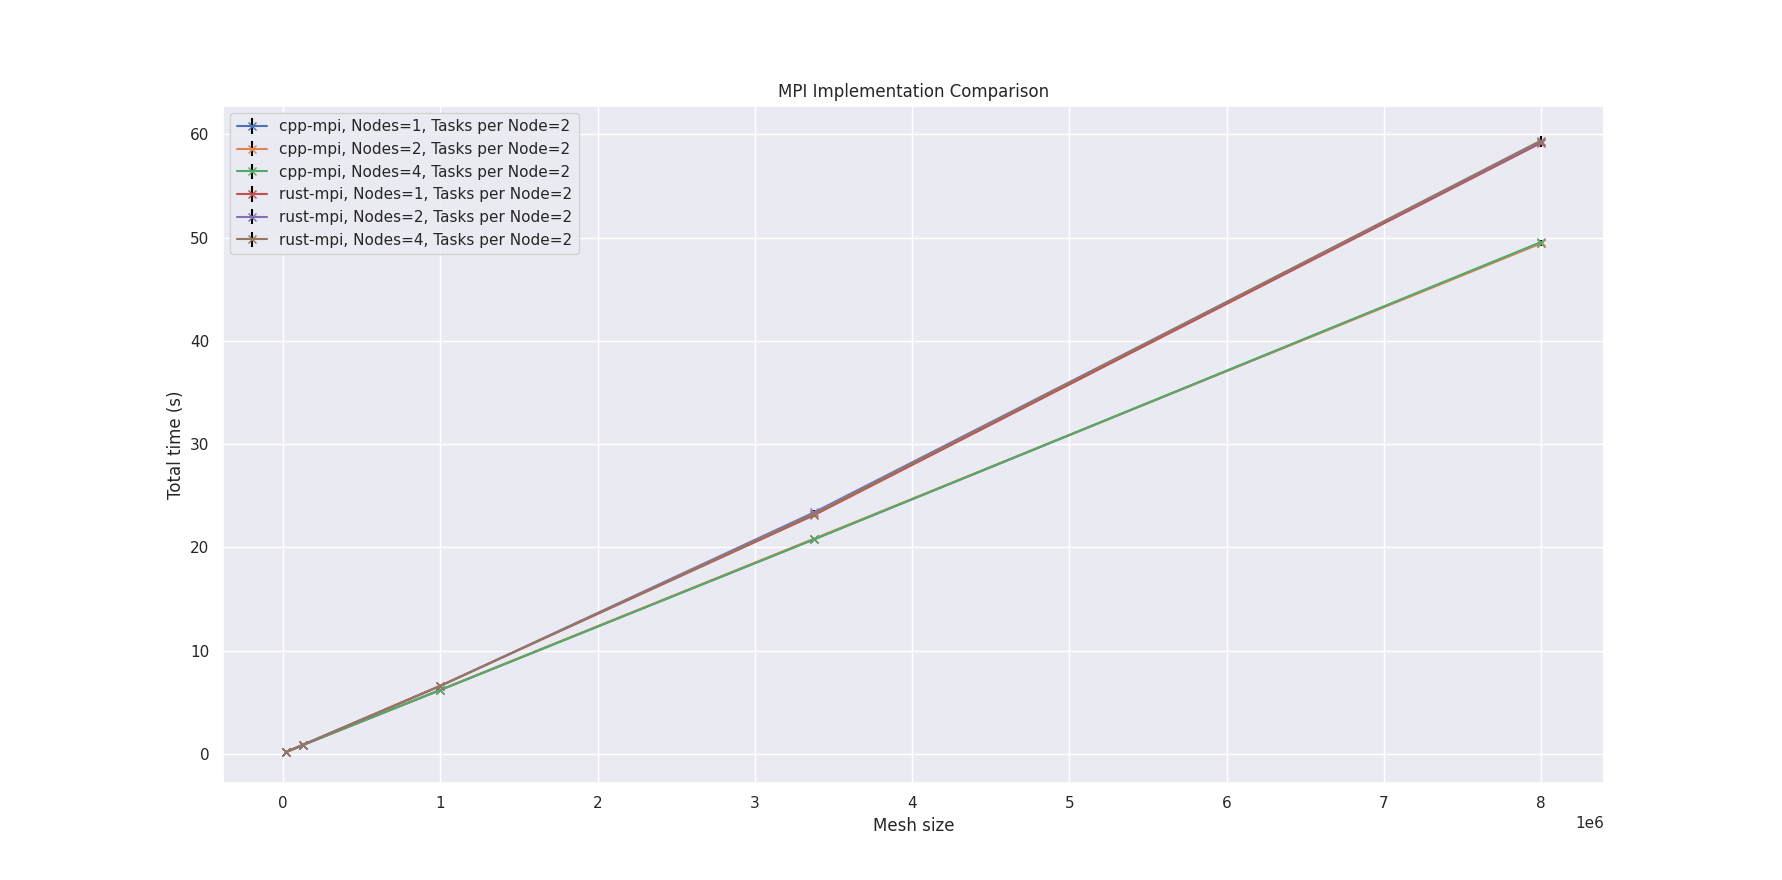
\includegraphics[width=\textwidth]{images/5_performance/parallelism/9_mpi_line.png}
    \caption{A line plot comparing the total wall times across all computational kernels for MPI Rust and C++ implementations of HPCCG.}
    \label{fig:9_mpi_line}
\end{figure}

\begin{figure}[H]
    \centering
    % This file was created with tikzplotlib v0.10.1.
\begin{tikzpicture}

\definecolor{darkorange25512714}{RGB}{255,127,14}
\definecolor{darkslategray38}{RGB}{38,38,38}
\definecolor{lightgray204}{RGB}{204,204,204}
\definecolor{steelblue31119180}{RGB}{31,119,180}

\begin{axis}[
axis line style={lightgray204},
height=0.45\textheight,
legend cell align={left},
legend style={
  fill opacity=0.8,
  draw opacity=1,
  text opacity=1,
  at={(0.03,0.97)},
  anchor=north west,
  draw=none
},
tick align=outside,
tick pos=left,
title={MPI Implementation Relative Execution Times},
width=\textwidth,
x grid style={lightgray204},
xlabel=\textcolor{darkslategray38}{Mesh size},
xmajorgrids,
xmin=-3183593.75, xmax=67199218.75,
xtick style={color=darkslategray38},
xtick={-10000000,0,10000000,20000000,30000000,40000000,50000000,60000000,70000000},
xticklabels={\ensuremath{-}1,0,1,2,3,4,5,6,7},
y grid style={lightgray204},
ylabel=\textcolor{darkslategray38}{Execution time relative to C++},
ymajorgrids,
ymin=0.978334672851017, ymax=1.45497187012864,
ytick style={color=darkslategray38}
]
\path [draw=black, semithick]
(axis cs:15625,1)
--(axis cs:15625,1);

\path [draw=black, semithick]
(axis cs:125000,1)
--(axis cs:125000,1);

\path [draw=black, semithick]
(axis cs:1000000,1)
--(axis cs:1000000,1);

\path [draw=black, semithick]
(axis cs:8000000,1)
--(axis cs:8000000,1);

\path [draw=black, semithick]
(axis cs:27000000,1)
--(axis cs:27000000,1);

\path [draw=black, semithick]
(axis cs:64000000,1)
--(axis cs:64000000,1);

\path [draw=black, semithick]
(axis cs:15625,1.07609152784119)
--(axis cs:15625,1.14961299360423);

\path [draw=black, semithick]
(axis cs:125000,1.01974672721846)
--(axis cs:125000,1.04945558277112);

\path [draw=black, semithick]
(axis cs:1000000,1.05850736021781)
--(axis cs:1000000,1.07392284442563);

\path [draw=black, semithick]
(axis cs:8000000,1.19560692314718)
--(axis cs:8000000,1.19893943343814);

\path [draw=black, semithick]
(axis cs:27000000,1.19602129682002)
--(axis cs:27000000,1.20141281406939);

\path [draw=black, semithick]
(axis cs:64000000,1.39968045169838)
--(axis cs:64000000,1.43330654297966);

\addplot [semithick, steelblue31119180, mark=x, mark size=3, mark options={solid}]
table {%
15625 1
125000 1
1000000 1
8000000 1
27000000 1
64000000 1
};
\addlegendentry{Baseline C++ with MPI}
\addplot [semithick, darkorange25512714, mark=x, mark size=3, mark options={solid}]
table {%
15625 1.11285221576691
125000 1.03460121154785
1000000 1.06621515750885
8000000 1.19727313518524
27000000 1.19871699810028
64000000 1.41649353504181
};
\addlegendentry{Relative Rust with MPI}
\end{axis}

\end{tikzpicture}

    \vspace*{-0.5cm}
    % 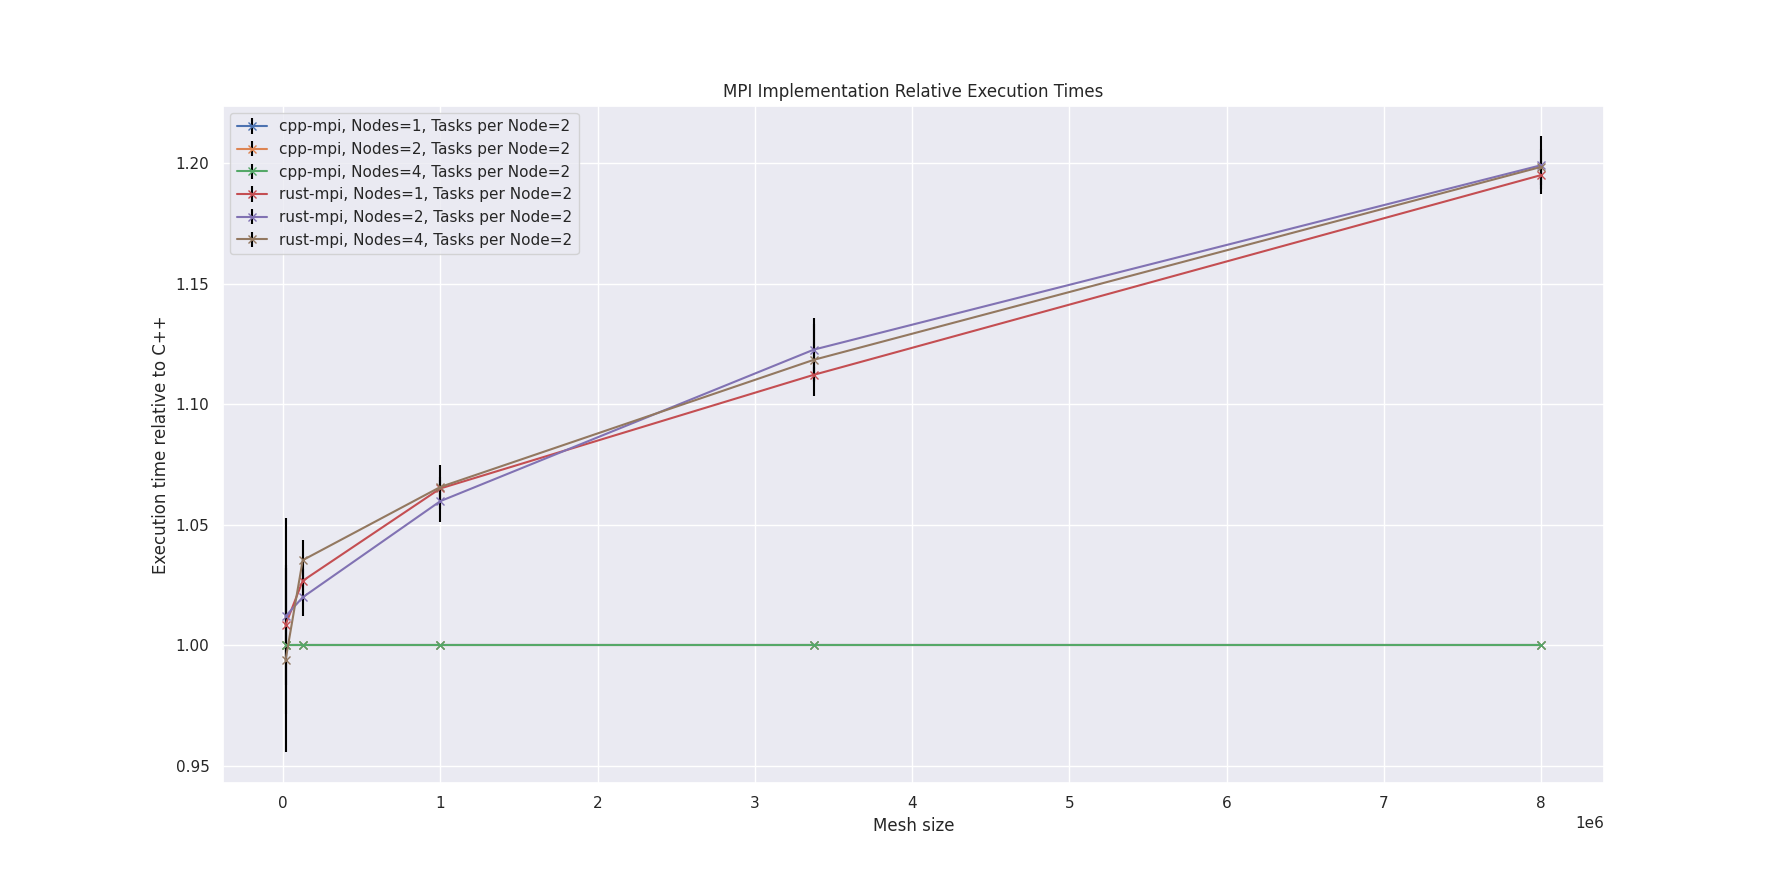
\includegraphics[width=\textwidth]{images/5_performance/parallelism/10_mpi_line_relative.png}
    \caption{A line plot comparing the total wall times relative to the MPI C++ implementation of HPCCG.}
    \label{fig:10_mpi_line_relative}
\end{figure}

From Figure \ref{fig:10_mpi_line_relative} which shows execution time relative to C++, we can see that for small meshes the Rust implementation is very similar in performance to the C++ implementation, with the $50 \times 50 \times 50$ mesh being only $1.035 \pm 0.015 \times$ slower. However, as the mesh size grows, the relative execution time also increases in steps. This may be as a result of batching or caching properties in the MPI network communication, resulting in plateaus as they saturate, followed by sudden jumps. 
% TODO: large run with this turned up, then reference it here. (this is hybrid I think...)

In summary, Rust remains performant in message passing workloads, but again trails C++ in performance for large, highly parallel workloads. The final recorded slow-down of Rust for the $400 \times 400 \times 400$ mesh was $1.416 \pm 0.017$, however it is not clear if this has converged, so large meshes may slow down further.
% The results from runs on Avon match those from those shown above on Kudu, with the slowdown across threads similarly converging at around $$.

% \subsection{MPI with Multi-threading}
% \label{ssec:mpi-multithreading}

% Shared and distributed memory parallelism can be used in tandem, with multi-threading within machines, which then communicate with each other through message passing. This allows programmers to leverage desirable properties from both approaches, such as the low-overhead performance of multi-threading in combination with the scalability of message passing.

% This assessment shows a compares a best-case scenario for MPI with Multi-threading, which best characterises a likely use case in High-Performance Computing. Four nodes are used, with one task per node, and 32 threads per task. As such, four MPI ranks are used in combination with 32 threads for a total parallelism degree of 128 concurrent execution paths. This configuration was then driven over the same test range as MPI, from $25 \times 25 \times 25$ to $250 \times 250 \times 250$, incrementing each axis size first by $25$, then by $50$ each time. This is again constrained by the \texttt{max\_external} constant in the reference implementation. The results of these experiments are shown in Figures \ref{fig:12_hybrid_line} and \ref{fig:13_hybrid_line_relative}.

% \begin{figure}[H]
%     \centering
%     % This file was created with tikzplotlib v0.10.1.
\begin{tikzpicture}

\definecolor{darkorange25512714}{RGB}{255,127,14}
\definecolor{darkslategray38}{RGB}{38,38,38}
\definecolor{lightgray204}{RGB}{204,204,204}
\definecolor{steelblue31119180}{RGB}{31,119,180}

\begin{axis}[
axis line style={lightgray204},
height=0.45\textheight,
legend cell align={left},
legend style={
  fill opacity=0.8,
  draw opacity=1,
  text opacity=1,
  at={(0.03,0.97)},
  anchor=north west,
  draw=none
},
tick align=outside,
tick pos=left,
title={MPI \& Multi-Threading Implementation Comparison},
width=\textwidth,
x grid style={lightgray204},
xlabel=\textcolor{darkslategray38}{Mesh size},
xmajorgrids,
xmin=-3183593.75, xmax=67199218.75,
xtick style={color=darkslategray38},
xtick={-10000000,0,10000000,20000000,30000000,40000000,50000000,60000000,70000000},
xticklabels={\ensuremath{-}1,0,1,2,3,4,5,6,7},
y grid style={lightgray204},
ylabel=\textcolor{darkslategray38}{Total time (s)},
ymajorgrids,
ymin=-17.5953972495309, ymax=374.400921378151,
ytick style={color=darkslategray38}
]
\path [draw=black, semithick]
(axis cs:15625,0.222617233545583)
--(axis cs:15625,0.226623266454417);

\path [draw=black, semithick]
(axis cs:125000,0.721052532281246)
--(axis cs:125000,0.725300967718754);

\path [draw=black, semithick]
(axis cs:1000000,4.61112797315782)
--(axis cs:1000000,4.62086702684218);

\path [draw=black, semithick]
(axis cs:8000000,35.7003613834714)
--(axis cs:8000000,36.0353386165286);

\path [draw=black, semithick]
(axis cs:27000000,120.412601321536)
--(axis cs:27000000,120.672398678464);

\path [draw=black, semithick]
(axis cs:64000000,286.567815433076)
--(axis cs:64000000,287.158684566924);

\path [draw=black, semithick]
(axis cs:15625,10.8911762003203)
--(axis cs:15625,11.2027237996798);

\path [draw=black, semithick]
(axis cs:125000,13.5414845686542)
--(axis cs:125000,14.0319654313458);

\path [draw=black, semithick]
(axis cs:1000000,25.0645393107993)
--(axis cs:1000000,25.4677606892007);

\path [draw=black, semithick]
(axis cs:8000000,68.0706090195893)
--(axis cs:8000000,68.4422909804107);

\path [draw=black, semithick]
(axis cs:27000000,168.193035189961)
--(axis cs:27000000,168.777014810039);

\path [draw=black, semithick]
(axis cs:64000000,355.403193104926)
--(axis cs:64000000,356.582906895074);

\addplot [semithick, steelblue31119180, mark=x, mark size=3, mark options={solid}]
table {%
15625 0.224620223045349
125000 0.723176717758179
1000000 4.61599731445312
8000000 35.8678512573242
27000000 120.542503356934
64000000 286.863250732422
};
\addlegendentry{C++ with MPI and OpenMP}
\addplot [semithick, darkorange25512714, mark=x, mark size=3, mark options={solid}]
table {%
15625 11.046950340271
125000 13.7867250442505
1000000 25.266149520874
8000000 68.2564468383789
27000000 168.48503112793
64000000 355.993041992188
};
\addlegendentry{Rust with MPI and OpenMP}
\end{axis}

\end{tikzpicture}

%     \vspace*{-0.5cm}
%     % 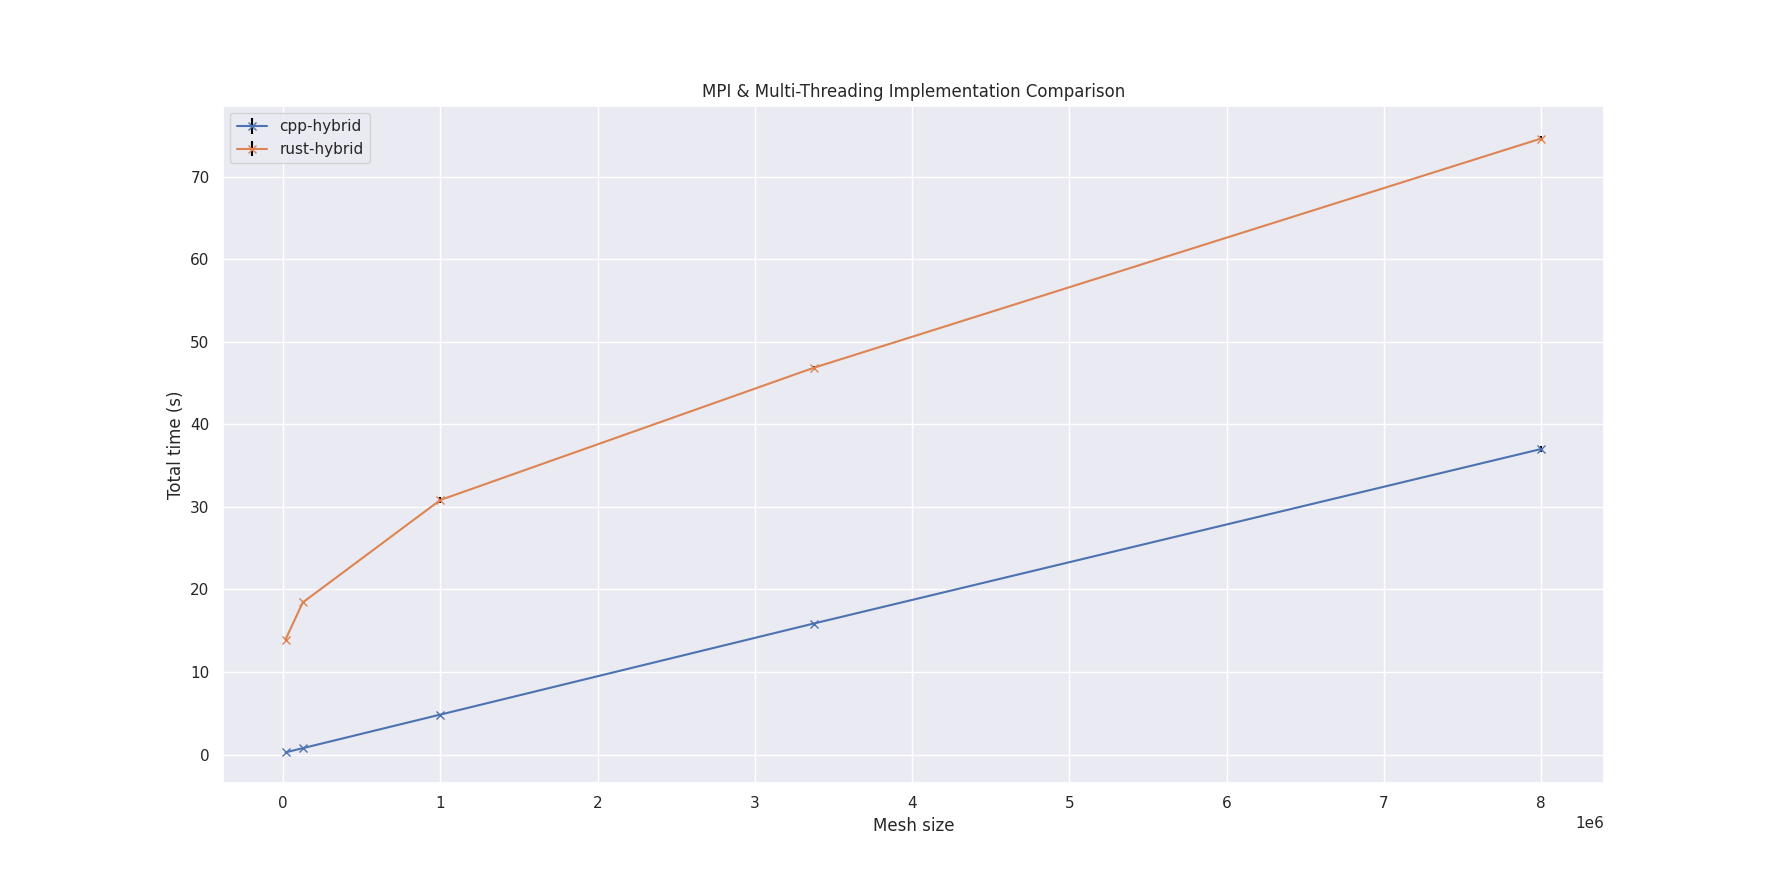
\includegraphics[width=\textwidth]{images/5_performance/parallelism/12_hybrid_line.png}
%     \caption{.}
%     \label{fig:12_hybrid_line}
% \end{figure}

% \begin{figure}[H]
%     \centering
%     % This file was created with tikzplotlib v0.10.1.
\begin{tikzpicture}

\definecolor{darkorange25512714}{RGB}{255,127,14}
\definecolor{darkslategray38}{RGB}{38,38,38}
\definecolor{lightgray204}{RGB}{204,204,204}
\definecolor{steelblue31119180}{RGB}{31,119,180}

\begin{axis}[
axis line style={lightgray204},
height=0.45\textheight,
legend cell align={left},
legend style={fill opacity=0.8, draw opacity=1, text opacity=1, draw=none},
tick align=outside,
tick pos=left,
title={MPI \& Multi-Threading Implementation Relative Execution Times},
width=\textwidth,
x grid style={lightgray204},
xlabel=\textcolor{darkslategray38}{Mesh size},
xmajorgrids,
xmin=-3183593.75, xmax=67199218.75,
xtick style={color=darkslategray38},
xtick={-10000000,0,10000000,20000000,30000000,40000000,50000000,60000000,70000000},
xticklabels={\ensuremath{-}1,0,1,2,3,4,5,6,7},
y grid style={lightgray204},
ylabel=\textcolor{darkslategray38}{Execution time relative to C++},
ymajorgrids,
ymin=-1.45005474091907, ymax=52.4511495593005,
ytick style={color=darkslategray38}
]
\path [draw=black, semithick]
(axis cs:15625,1)
--(axis cs:15625,1);

\path [draw=black, semithick]
(axis cs:125000,1)
--(axis cs:125000,1);

\path [draw=black, semithick]
(axis cs:1000000,1)
--(axis cs:1000000,1);

\path [draw=black, semithick]
(axis cs:8000000,1)
--(axis cs:8000000,1);

\path [draw=black, semithick]
(axis cs:27000000,1)
--(axis cs:27000000,1);

\path [draw=black, semithick]
(axis cs:64000000,1)
--(axis cs:64000000,1);

\path [draw=black, semithick]
(axis cs:15625,48.3600280100368)
--(axis cs:15625,50.0010948183814);

\path [draw=black, semithick]
(axis cs:125000,18.7204075551941)
--(axis cs:125000,19.4078231989058);

\path [draw=black, semithick]
(axis cs:1000000,5.42954909748842)
--(axis cs:1000000,5.51766220407749);

\path [draw=black, semithick]
(axis cs:8000000,1.89271164598645)
--(axis cs:8000000,1.91328453164895);

\path [draw=black, semithick]
(axis cs:27000000,1.39487060053773)
--(axis cs:27000000,1.4005754039835);

\path [draw=black, semithick]
(axis cs:64000000,1.2385641477104)
--(axis cs:64000000,1.24340626850708);

\addplot [semithick, steelblue31119180, mark=x, mark size=3, mark options={solid}]
table {%
15625 1
125000 1
1000000 1
8000000 1
27000000 1
64000000 1
};
\addlegendentry{C++ with MPI and OpenMP}
\addplot [semithick, darkorange25512714, mark=x, mark size=3, mark options={solid}]
table {%
15625 49.1805610656738
125000 19.064115524292
1000000 5.47360563278198
8000000 1.90299808979034
27000000 1.39772295951843
64000000 1.24098515510559
};
\addlegendentry{Rust with MPI and OpenMP}
\end{axis}

\end{tikzpicture}

%     \vspace*{-0.5cm}
%     % 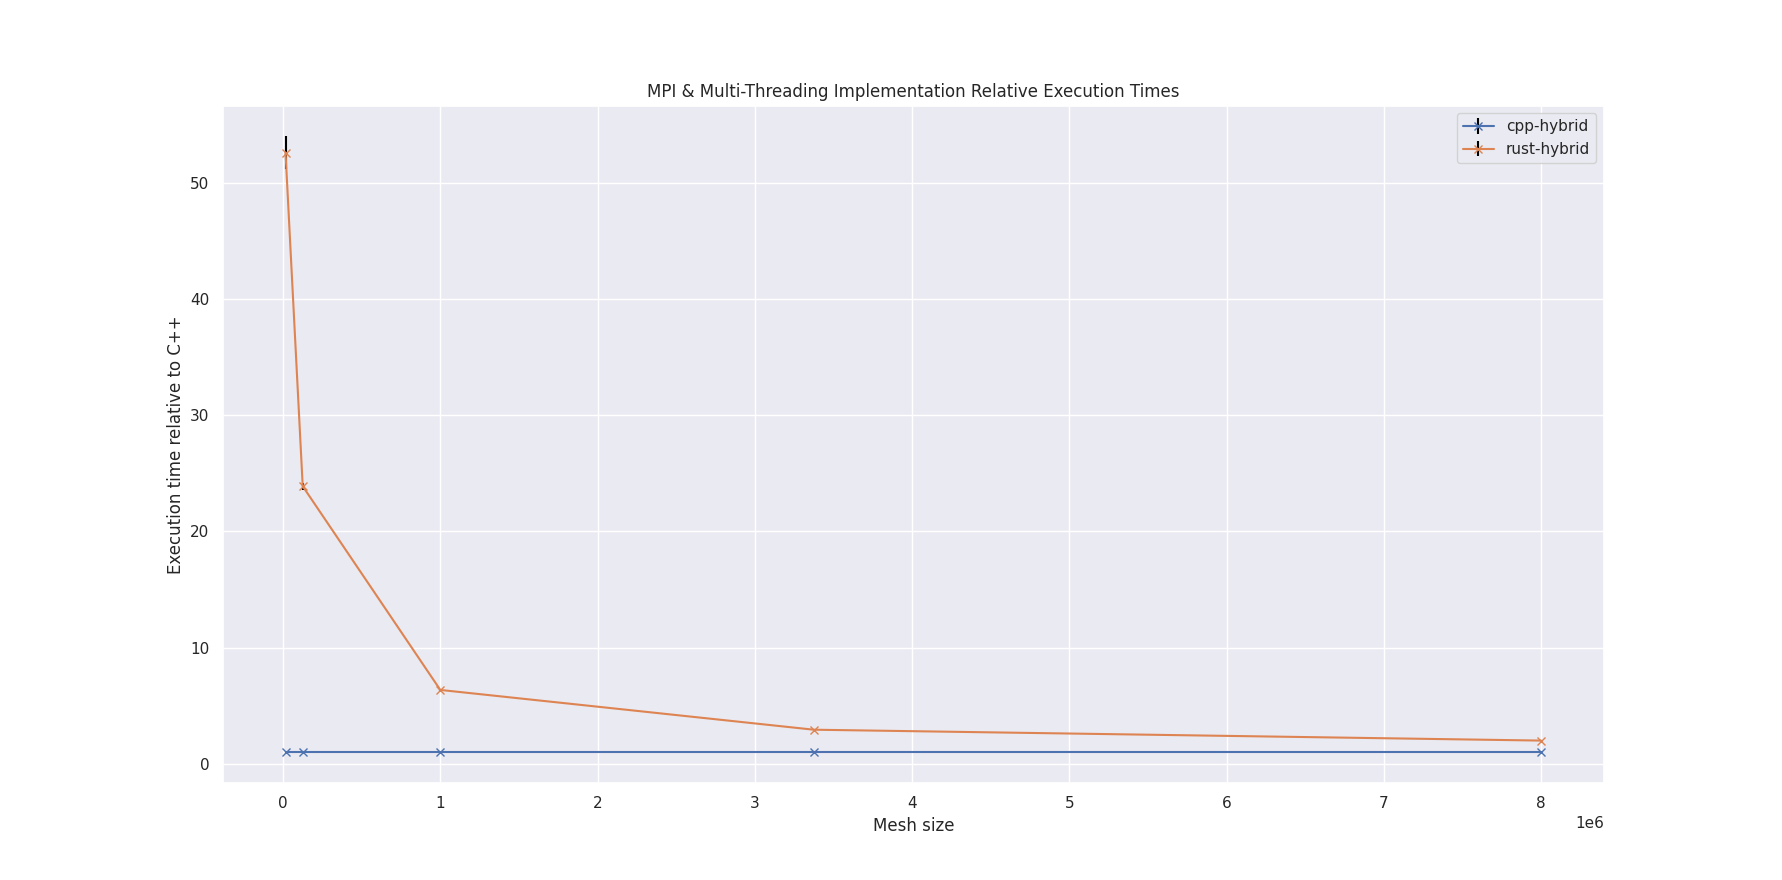
\includegraphics[width=\textwidth]{images/5_performance/parallelism/13_hybrid_line_relative.png}
%     \caption{.}
%     \label{fig:13_hybrid_line_relative}
% \end{figure}

% % Analysis
% In summary,

\subsection{Performance portability frameworks}
\label{ssec:performance-portability-frameworks-results}

Finally, performance portability frameworks, such as Kokkos \cite{KokkosEcosystem}, are commonly used within High-Performance Computing to allow writing software which can run across a variety of hardware. However, such frameworks often incur a performance cost over hand-optimised implementations targeted at specific hardware. The fact that these frameworks are common, despite this performance cost, motivates the idea that Rust could be suitable for High-Performance Computing as a result of its productivity benefits, despite its performance impact.

This assessment compares the Rust, Kokkos, and C++ executables performance over a range of mesh sizes, from $25 \times 25 \times 25$ to $400 \times 400 \times 400$, incrementing each axis size first by $25$, then $50$, then $100$ for the remaining increments. As with the parallel assessment, a single node and a single task per node is used, and the implementations are compared with 32 threads each. The results of these experiments are shown in Figures \ref{fig:16_kokkos_line} and \ref{fig:17_kokkos_line_relative}.

\begin{figure}[H]
    \centering
    % This file was created with tikzplotlib v0.10.1.
\begin{tikzpicture}

\definecolor{darkorange25512714}{RGB}{255,127,14}
\definecolor{darkslategray38}{RGB}{38,38,38}
\definecolor{forestgreen4416044}{RGB}{44,160,44}
\definecolor{lightgray204}{RGB}{204,204,204}
\definecolor{steelblue31119180}{RGB}{31,119,180}

\begin{axis}[
axis line style={lightgray204},
height=0.375\textheight,
legend cell align={left},
legend style={
  fill opacity=0.8,
  draw opacity=1,
  text opacity=1,
  at={(0.03,0.97)},
  anchor=north west,
  % draw=none
},
tick align=outside,
tick pos=left,
title={C++, Kokkos, and Rust with Multi-Threading Version Comparison},
width=\textwidth,
x grid style={lightgray204},
xlabel=\textcolor{darkslategray38}{Mesh size},
xmajorgrids,
xmin=-3183593.75, xmax=67199218.75,
xtick style={color=darkslategray38},
xtick={-10000000,0,10000000,20000000,30000000,40000000,50000000,60000000,70000000},
xticklabels={\ensuremath{-}1,0,1,2,3,4,5,6,7},
y grid style={lightgray204},
ylabel=\textcolor{darkslategray38}{Total time (s)},
ymajorgrids,
ymin=-4.23790328040092, ymax=89.3730856388962,
ytick style={color=darkslategray38}
]
\path [draw=black, semithick]
(axis cs:125000,0.0784584465659017)
--(axis cs:125000,0.144491553434098);

\path [draw=black, semithick]
(axis cs:1000000,2.09968166972454)
--(axis cs:1000000,2.20959833027546);

\path [draw=black, semithick]
(axis cs:8000000,9.34541000342519)
--(axis cs:8000000,10.2206649965748);

\path [draw=black, semithick]
(axis cs:27000000,23.069681985023)
--(axis cs:27000000,24.087418014977);

\path [draw=black, semithick]
(axis cs:64000000,52.093447132533)
--(axis cs:64000000,53.282652867467);

\path [draw=black, semithick]
(axis cs:125000,0.314281244848337)
--(axis cs:125000,0.326918755151663);

\path [draw=black, semithick]
(axis cs:1000000,1.53788009399903)
--(axis cs:1000000,1.55631990600097);

\path [draw=black, semithick]
(axis cs:8000000,11.7373268542365)
--(axis cs:8000000,11.8164231457635);

\path [draw=black, semithick]
(axis cs:27000000,36.6417225194371)
--(axis cs:27000000,36.7492274805629);

\path [draw=black, semithick]
(axis cs:64000000,84.7252093119809)
--(axis cs:64000000,85.1180406880191);

\path [draw=black, semithick]
(axis cs:125000,0.125948579736594)
--(axis cs:125000,0.130024420263406);

\path [draw=black, semithick]
(axis cs:1000000,1.38150993061621)
--(axis cs:1000000,1.62775506938379);

\path [draw=black, semithick]
(axis cs:8000000,7.42827748173787)
--(axis cs:8000000,7.99833251826213);

\path [draw=black, semithick]
(axis cs:27000000,22.1963451938929)
--(axis cs:27000000,22.6153048061071);

\path [draw=black, semithick]
(axis cs:64000000,53.8656584151548)
--(axis cs:64000000,54.5794415848452);

\addplot [semithick, steelblue31119180, mark=x, mark size=3, mark options={solid}]
table {%
125000 0.111474990844727
1000000 2.15463995933533
8000000 9.78303718566895
27000000 23.5785503387451
64000000 52.6880493164062
};
\addlegendentry{C++ with OpenMP}
\addplot [semithick, darkorange25512714, mark=triangle, mark size=3, mark options={solid}]
table {%
125000 0.320600032806396
1000000 1.54709994792938
8000000 11.7768745422363
27000000 36.6954765319824
64000000 84.9216232299805
};
\addlegendentry{Rust with Rayon}
\addplot [semithick, forestgreen4416044, mark=star, mark size=3, mark options={solid}]
table {%
125000 0.127986550331116
1000000 1.50463247299194
8000000 7.71330499649048
27000000 22.4058246612549
64000000 54.2225494384766
};
\addlegendentry{C++ with Kokkos}
\end{axis}

\end{tikzpicture}

    \vspace*{-0.5cm}
    % 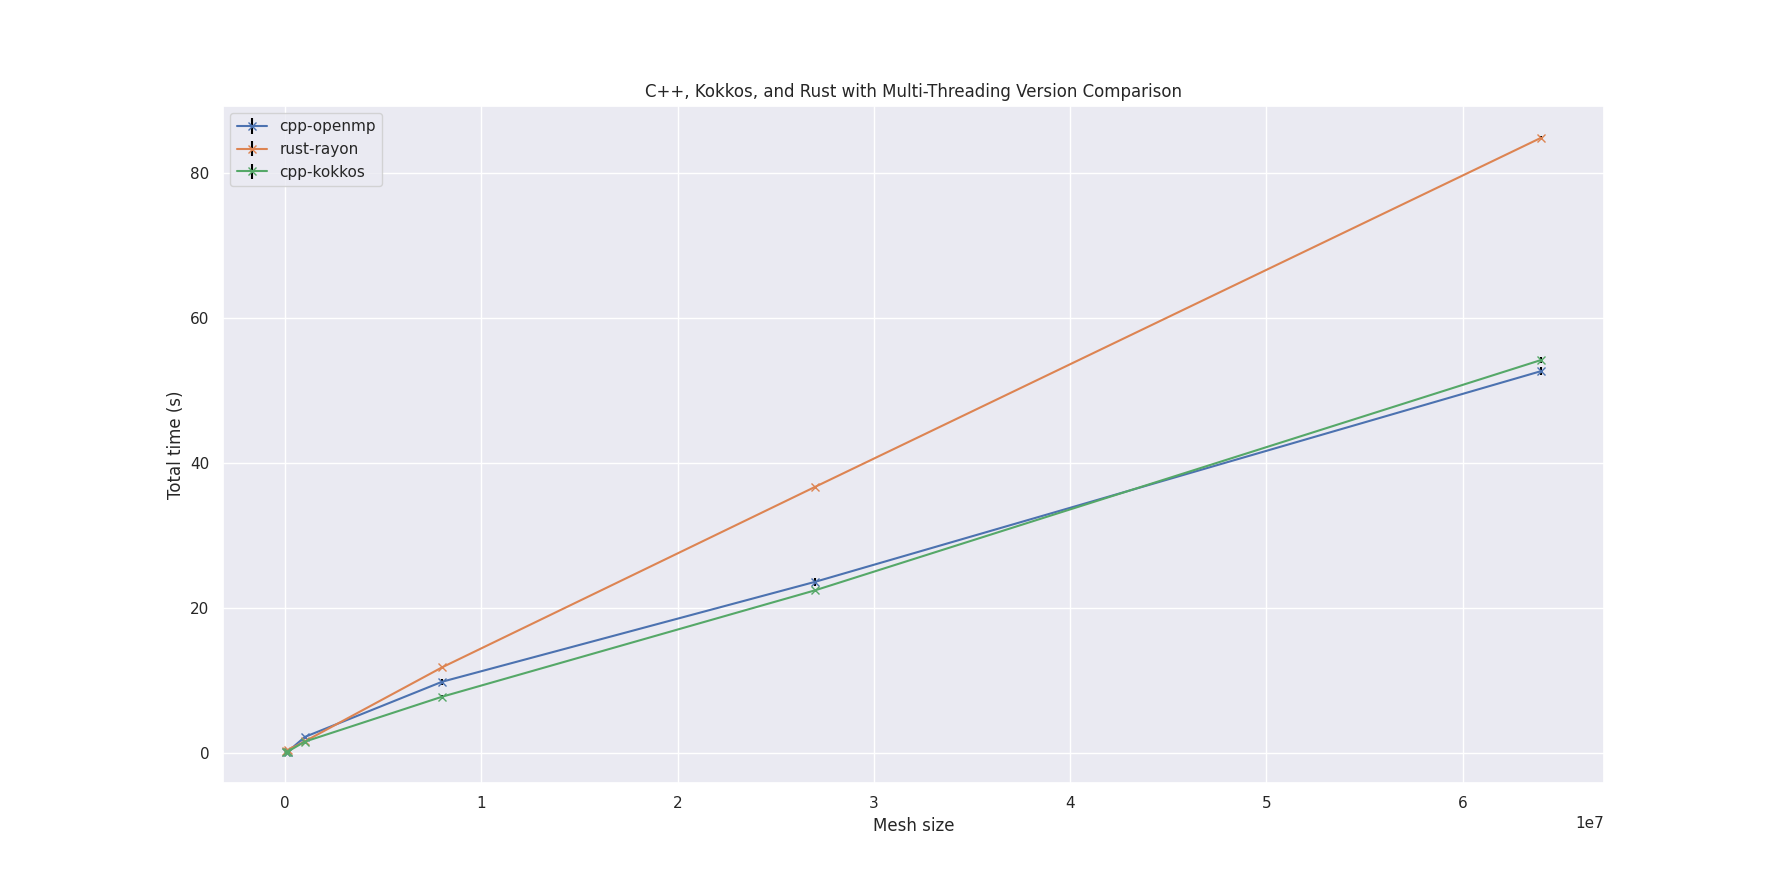
\includegraphics[width=\textwidth]{images/5_performance/parallelism/16_kokkos_line.png}
    \caption{A line plot comparing the total wall times across all computational kernels for multithreaded Kokkos, Rust, and C++ implementations of HPCCG.}
    \label{fig:16_kokkos_line}
\end{figure}

\begin{figure}[H]
    \centering
    % This file was created with tikzplotlib v0.10.1.
\begin{tikzpicture}

\definecolor{darkorange25512714}{RGB}{255,127,14}
\definecolor{darkslategray38}{RGB}{38,38,38}
\definecolor{forestgreen4416044}{RGB}{44,160,44}
\definecolor{lightgray204}{RGB}{204,204,204}
\definecolor{steelblue31119180}{RGB}{31,119,180}

\begin{axis}[
axis line style={lightgray204},
height=0.375\textheight,
legend cell align={left},
legend style={fill opacity=0.8, draw opacity=1, text opacity=1}, %, draw=none},
tick align=outside,
tick pos=left,
title={C++, Kokkos, and Rust with Multi-Threading Relative Execution Times},
width=\textwidth,
x grid style={lightgray204},
xlabel=\textcolor{darkslategray38}{Mesh size},
xmajorgrids,
xmin=-3183593.75, xmax=67199218.75,
xtick style={color=darkslategray38},
xtick={-10000000,0,10000000,20000000,30000000,40000000,50000000,60000000,70000000},
xticklabels={\ensuremath{-}1,0,1,2,3,4,5,6,7},
y grid style={lightgray204},
ylabel=\textcolor{darkslategray38}{Execution time relative to C++},
ymajorgrids,
ymin=0.258566750026608, ymax=4.1919184562473,
ytick style={color=darkslategray38}
]

\path [draw=black, semithick]
(axis cs:125000,1)
--(axis cs:125000,1);

\path [draw=black, semithick]
(axis cs:1000000,1)
--(axis cs:1000000,1);

\path [draw=black, semithick]
(axis cs:8000000,1)
--(axis cs:8000000,1);

\path [draw=black, semithick]
(axis cs:27000000,1)
--(axis cs:27000000,1);

\path [draw=black, semithick]
(axis cs:64000000,1)
--(axis cs:64000000,1);

\path [draw=black, semithick]
(axis cs:125000,2.02229205258536)
--(axis cs:125000,3.72967027080554);

\path [draw=black, semithick]
(axis cs:1000000,0.699223725727002)
--(axis cs:1000000,0.736839839416131);

\path [draw=black, semithick]
(axis cs:8000000,1.14980385525892)
--(axis cs:8000000,1.25780727778641);

\path [draw=black, semithick]
(axis cs:27000000,1.52264230819383)
--(axis cs:27000000,1.58997275931456);

\path [draw=black, semithick]
(axis cs:64000000,1.59321391949516)
--(axis cs:64000000,1.63034910855389);

\path [draw=black, semithick]
(axis cs:125000,0.807578794564784)
--(axis cs:125000,1.48865802983531);

\path [draw=black, semithick]
(axis cs:1000000,0.638467242534317)
--(axis cs:1000000,0.758176744396214);

\path [draw=black, semithick]
(axis cs:8000000,0.742689827067916)
--(axis cs:8000000,0.834183408877464);

\path [draw=black, semithick]
(axis cs:27000000,0.927912974658666)
--(axis cs:27000000,0.972613139118474);

\path [draw=black, semithick]
(axis cs:64000000,1.01567924576466)
--(axis cs:64000000,1.04256925650483);

\addplot [semithick, steelblue31119180, mark=x, mark size=3, mark options={solid}]
table {%
125000 1
1000000 1
8000000 1
27000000 1
64000000 1
};
\addlegendentry{Baseline C++ with OpenMP}
\addplot [semithick, darkorange25512714, mark=triangle, mark size=3, mark options={solid}]
table {%
125000 2.875981092453
1000000 0.718031764030457
8000000 1.20380556583405
27000000 1.556307554245
64000000 1.61178147792816
};
\addlegendentry{Relative Rust with Rayon}
\addplot [semithick, forestgreen4416044, mark=star, mark size=3, mark options={solid}]
table {%
125000 1.14811837673187
1000000 0.698322057723999
8000000 0.788436651229858
27000000 0.950263023376465
64000000 1.02912425994873
};
\addlegendentry{Relative C++ with Kokkos}
\end{axis}

\end{tikzpicture}

    \vspace*{-0.5cm}
    % 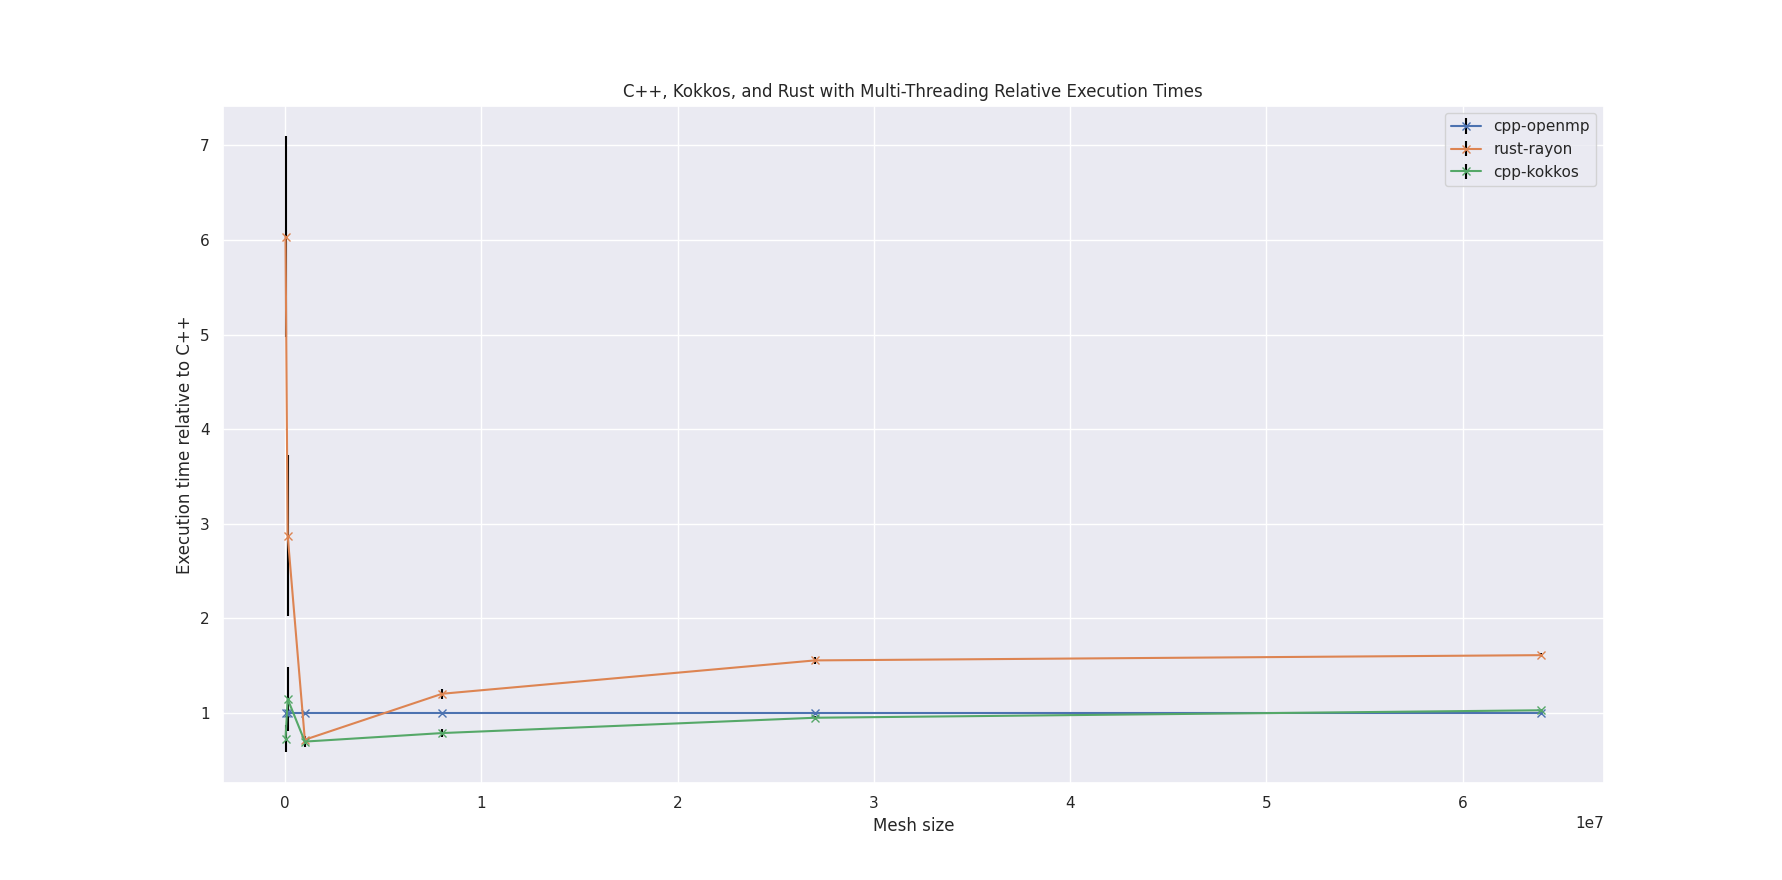
\includegraphics[width=\textwidth]{images/5_performance/parallelism/17_kokkos_line_relative.png}
    \caption{A line plot comparing the Rust and Kokkos total wall times relative to the multithreaded C++ implementation of HPCCG.}
    \label{fig:17_kokkos_line_relative}
\end{figure}


From Figure \ref{fig:16_kokkos_line} which shows execution time of the Rust and Kokkos implementations, relative to C++. Here, we can see that Kokkos out-performs C++ for small mesh sizes, but as the mesh size grows begins to incur a performance cost beyond C++. From \ref{fig:17_kokkos_line_relative} we can quantitatively see that for the largest $400 \times 400 \times 400$ mesh, the Kokkos implementation has a $1.03 \pm 0.01 \times$ slow-down, and the Rust implementation has a $1.61 \pm 0.02 \times$ slow-down. 

In this set of results, the slow-down of Kokkos is not sufficiently comparable to that of Rust to motivate the performance-productivity trade-off. However, the benchmarked implementation uses Kokkos for parallelism only, without modifying the data structure, so may underreport the upper bound for the performance impact of Kokkos. This performance impact was previously explored in Edwards, Trott, and Sunderland's 2014 paper ``Kokkos: Enabling manycore performance portability through polymorphic memory access patterns''. In this paper, they conclude that ``mini-applications that achieve at least 90\% of the performance of architecture specific, optimized variants'' \cite{carteredwardsKokkosEnablingManycore2014} when applied to MiniMD, another mini-app in the Mantevo suite. From this we can see that Edwards, Trott, and Sunderland's results indicate a worst case $1.11 \times$ slowdown for Kokkos applied to MiniMD, which is much closer to the measured $1.61 \pm 0.02 \times$ slow-down recorded for the Rust translation of HPCCG.


\section{Summary of results}
\label{sec:performance-results}

Having compared the performance of individual parallelism approaches between C++ and Rust implementations, we can finally get an overall view of performance through a comparison between the approaches for each of the languages. Figure \ref{fig:translation_parallelism_rust} shows the relative performance as characterised by the scaling of total wall time for serial, multithreaded, MPI, and hybrid Rust translations of the HPCCG mini-app.

\begin{figure}[H]
    \centering
    % This file was created with tikzplotlib v0.10.1.
\begin{tikzpicture}

\definecolor{crimson2143940}{RGB}{214,39,40}
\definecolor{darkorange25512714}{RGB}{255,127,14}
\definecolor{darkslategray38}{RGB}{38,38,38}
\definecolor{forestgreen4416044}{RGB}{44,160,44}
\definecolor{lightgray204}{RGB}{204,204,204}
\definecolor{steelblue31119180}{RGB}{31,119,180}

\begin{axis}[
axis line style={lightgray204},
height=0.45\textheight,
legend cell align={left},
legend style={
  fill opacity=0.8,
  draw opacity=1,
  text opacity=1,
  at={(0.03,0.97)},
  anchor=north west,
  draw=none
},
tick align=outside,
tick pos=left,
title={Rust Parallelism Total Times},
width=\textwidth,
x grid style={lightgray204},
xlabel=\textcolor{darkslategray38}{Mesh size},
xmajorgrids,
xmin=-136718.75, xmax=5621093.75,
xtick style={color=darkslategray38},
xtick={-1000000,0,1000000,2000000,3000000,4000000,5000000,6000000},
xticklabels={\ensuremath{-}1,0,1,2,3,4,5,6},
y grid style={lightgray204},
ylabel=\textcolor{darkslategray38}{Total time (s)},
ymajorgrids,
ymin=-1.82808433539877, ymax=45.1943113894709,
ytick style={color=darkslategray38}
]
\path [draw=black, semithick]
(axis cs:125000,0.779656118982615)
--(axis cs:125000,0.789693881017385);

\path [draw=black, semithick]
(axis cs:421875,2.55632164214235)
--(axis cs:421875,2.62382835785765);

\path [draw=black, semithick]
(axis cs:1000000,6.19294376900195)
--(axis cs:1000000,6.35945623099805);

\path [draw=black, semithick]
(axis cs:1953125,12.5751891928374)
--(axis cs:1953125,12.7739108071626);

\path [draw=black, semithick]
(axis cs:3375000,21.6653043770414)
--(axis cs:3375000,21.9961456229586);

\path [draw=black, semithick]
(axis cs:5359375,40.557258493516)
--(axis cs:5359375,41.209291506484);

\path [draw=black, semithick]
(axis cs:125000,0.309297288458942)
--(axis cs:125000,0.316752711541057);

\path [draw=black, semithick]
(axis cs:421875,0.759112258047775)
--(axis cs:421875,0.775687741952225);

\path [draw=black, semithick]
(axis cs:1000000,1.54119986933917)
--(axis cs:1000000,1.55555013066083);

\path [draw=black, semithick]
(axis cs:1953125,2.80682390599246)
--(axis cs:1953125,2.84262609400754);

\path [draw=black, semithick]
(axis cs:3375000,4.66096039225482)
--(axis cs:3375000,4.73758960774518);

\path [draw=black, semithick]
(axis cs:5359375,8.06759300833981)
--(axis cs:5359375,8.28130699166019);

\path [draw=black, semithick]
(axis cs:125000,0.817391041076087)
--(axis cs:125000,0.822608958923913);

\path [draw=black, semithick]
(axis cs:421875,2.95001915537841)
--(axis cs:421875,2.99868084462159);

\path [draw=black, semithick]
(axis cs:1000000,7.0149363693974)
--(axis cs:1000000,7.0866636306026);

\path [draw=black, semithick]
(axis cs:1953125,13.7607447968126)
--(axis cs:1953125,13.9279552031874);

\path [draw=black, semithick]
(axis cs:3375000,25.0584615978647)
--(axis cs:3375000,25.3326384021353);

\path [draw=black, semithick]
(axis cs:5359375,42.6778202343868)
--(axis cs:5359375,43.0569297656132);

\path [draw=black, semithick]
(axis cs:125000,0.67392059088761)
--(axis cs:125000,0.68587940911239);

\path [draw=black, semithick]
(axis cs:421875,2.17840611609867)
--(axis cs:421875,2.18589388390133);

\path [draw=black, semithick]
(axis cs:1000000,5.09397316158006)
--(axis cs:1000000,5.17522683841994);

\path [draw=black, semithick]
(axis cs:1953125,10.0038666058921)
--(axis cs:1953125,10.0712833941079);

\path [draw=black, semithick]
(axis cs:3375000,18.4395198616569)
--(axis cs:3375000,18.6787801383431);

\path [draw=black, semithick]
(axis cs:5359375,30.9011331705115)
--(axis cs:5359375,31.1655668294885);

\addplot [semithick, steelblue31119180, mark=x, mark size=3, mark options={solid}]
table {%
125000 0.784675002098083
421875 2.59007501602173
1000000 6.27619981765747
1953125 12.6745500564575
3375000 21.8307247161865
5359375 40.8832740783691
};
\addlegendentry{Serial Rust}
\addplot [semithick, darkorange25512714, mark=x, mark size=3, mark options={solid}]
table {%
125000 0.313024997711182
421875 0.767400026321411
1000000 1.54837501049042
1953125 2.82472491264343
3375000 4.69927501678467
5359375 8.1744499206543
};
\addlegendentry{Rust with Rayon}
\addplot [semithick, forestgreen4416044, mark=x, mark size=3, mark options={solid}]
table {%
125000 0.819999933242798
421875 2.97434997558594
1000000 7.05079984664917
1953125 13.844349861145
3375000 25.1955509185791
5359375 42.867374420166
};
\addlegendentry{Rust with MPI}
\addplot [semithick, crimson2143940, mark=x, mark size=3, mark options={solid}]
table {%
125000 0.679899930953979
421875 2.18214988708496
1000000 5.1346001625061
1953125 10.0375747680664
3375000 18.5591506958008
5359375 31.0333499908447
};
\addlegendentry{Rust with MPI and Rayon}
\end{axis}

\end{tikzpicture}

    \vspace*{-0.5cm}
    \caption{A diagram showing the total wall time taken for Rust implementations of parallelism approaches, as the overall mesh size is varied.}
    \label{fig:translation_parallelism_rust}
\end{figure}

Here we can see that multi-threading is by far the most performant for small workloads on a single computer node. However, message passing approaches provide the capability to scale processing to clustered compute resources beyond the shared memory architecture of a single machine, and can be used in combination with multithreaded approaches.

Figure \ref{fig:translation_parallelism_cpp} shows the same experiments run over the parallelism methodologies of the C++ codebase. From this, we can see that very similar trends hold, with the only difference being the Rust MPI implementation is slightly slower. A likely cause for this is the overhead as a result of the Rust bindings into the C++ implementation of the MPI specification.

\begin{figure}[H]
    \centering
    % This file was created with tikzplotlib v0.10.1.
\begin{tikzpicture}

\definecolor{crimson2143940}{RGB}{214,39,40}
\definecolor{darkorange25512714}{RGB}{255,127,14}
\definecolor{darkslategray38}{RGB}{38,38,38}
\definecolor{forestgreen4416044}{RGB}{44,160,44}
\definecolor{lightgray204}{RGB}{204,204,204}
\definecolor{steelblue31119180}{RGB}{31,119,180}

\begin{axis}[
axis line style={lightgray204},
height=0.45\textheight,
legend cell align={left},
legend style={
  fill opacity=0.8,
  draw opacity=1,
  text opacity=1,
  at={(0.03,0.97)},
  anchor=north west,
  draw=none
},
tick align=outside,
tick pos=left,
title={C++ Parallelism Total Times},
width=\textwidth,
x grid style={lightgray204},
xlabel=\textcolor{darkslategray38}{Mesh size},
xmajorgrids,
xmin=-136718.75, xmax=5621093.75,
xtick style={color=darkslategray38},
xtick={-1000000,0,1000000,2000000,3000000,4000000,5000000,6000000},
xticklabels={\ensuremath{-}1,0,1,2,3,4,5,6},
y grid style={lightgray204},
ylabel=\textcolor{darkslategray38}{Total time (s)},
ymajorgrids,
ymin=-1.38292786946242, ymax=31.5790793512316,
ytick style={color=darkslategray38}
]
\path [draw=black, semithick]
(axis cs:125000,0.630818193843731)
--(axis cs:125000,0.646766306156269);

\path [draw=black, semithick]
(axis cs:421875,2.223066540468)
--(axis cs:421875,2.244373459532);

\path [draw=black, semithick]
(axis cs:1000000,5.35376867074015)
--(axis cs:1000000,5.46672132925985);

\path [draw=black, semithick]
(axis cs:1953125,10.6241993611994)
--(axis cs:1953125,10.8332506388006);

\path [draw=black, semithick]
(axis cs:3375000,18.7914397981746)
--(axis cs:3375000,18.9563102018254);

\path [draw=black, semithick]
(axis cs:5359375,29.6293416527015)
--(axis cs:5359375,29.8630583472985);

\path [draw=black, semithick]
(axis cs:125000,0.11534518602367)
--(axis cs:125000,0.12536881397633);

\path [draw=black, semithick]
(axis cs:421875,0.908496237202436)
--(axis cs:421875,0.922190262797564);

\path [draw=black, semithick]
(axis cs:1000000,1.6290644741359)
--(axis cs:1000000,2.2715155258641);

\path [draw=black, semithick]
(axis cs:1953125,3.70726366078273)
--(axis cs:1953125,4.04439133921727);

\path [draw=black, semithick]
(axis cs:3375000,5.02368443393088)
--(axis cs:3375000,5.47941556606912);

\path [draw=black, semithick]
(axis cs:5359375,6.86434211956473)
--(axis cs:5359375,7.68154788043527);

\path [draw=black, semithick]
(axis cs:125000,0.634065478044844)
--(axis cs:125000,0.636860021955156);

\path [draw=black, semithick]
(axis cs:421875,2.22843066465354)
--(axis cs:421875,2.24911433534646);

\path [draw=black, semithick]
(axis cs:1000000,5.38544308377665)
--(axis cs:1000000,5.41628691622335);

\path [draw=black, semithick]
(axis cs:1953125,10.6014728603183)
--(axis cs:1953125,10.7603771396817);

\path [draw=black, semithick]
(axis cs:3375000,18.6283197759457)
--(axis cs:3375000,18.9545802240543);

\path [draw=black, semithick]
(axis cs:5359375,29.5465437042545)
--(axis cs:5359375,30.0808062957455);

\path [draw=black, semithick]
(axis cs:125000,0.480264066421818)
--(axis cs:125000,0.484687433578182);

\path [draw=black, semithick]
(axis cs:421875,1.70470713896287)
--(axis cs:421875,1.72148786103713);

\path [draw=black, semithick]
(axis cs:1000000,4.08637942405161)
--(axis cs:1000000,4.12355057594839);

\path [draw=black, semithick]
(axis cs:1953125,8.21026577774712)
--(axis cs:1953125,8.26302422225288);

\path [draw=black, semithick]
(axis cs:3375000,14.3626018007787)
--(axis cs:3375000,14.4694981992213);

\path [draw=black, semithick]
(axis cs:5359375,22.8226756633978)
--(axis cs:5359375,23.0698243366022);

\addplot [semithick, steelblue31119180, mark=x, mark size=3, mark options={solid}]
table {%
125000 0.638792276382446
421875 2.23372006416321
1000000 5.41024494171143
1953125 10.7287254333496
3375000 18.8738746643066
5359375 29.7462005615234
};
\addlegendentry{Serial C++}
\addplot [semithick, darkorange25512714, mark=x, mark size=3, mark options={solid}]
table {%
125000 0.120357036590576
421875 0.915343284606934
1000000 1.9502899646759
1953125 3.87582755088806
3375000 5.25155019760132
5359375 7.27294492721558
};
\addlegendentry{C++ with OpenMP}
\addplot [semithick, forestgreen4416044, mark=x, mark size=3, mark options={solid}]
table {%
125000 0.635462760925293
421875 2.23877239227295
1000000 5.40086507797241
1953125 10.6809253692627
3375000 18.7914505004883
5359375 29.8136749267578
};
\addlegendentry{C++ with MPI}
\addplot [semithick, crimson2143940, mark=x, mark size=3, mark options={solid}]
table {%
125000 0.482475757598877
421875 1.71309745311737
1000000 4.10496520996094
1953125 8.23664474487305
3375000 14.4160499572754
5359375 22.9462509155273
};
\addlegendentry{C++ with MPI and OpenMP}
\end{axis}

\end{tikzpicture}

    \vspace*{-0.5cm}
    \caption{A diagram showing the total wall time taken for C++ implementations of parallelism approaches, as the overall mesh size is varied.}
    \label{fig:translation_parallelism_cpp}
\end{figure}

In summary, from the detailed comparisons in the previous sections we can see that Rust consistently approaches C++ in performance for representative High-Performance Computing workloads, with at worst around a $1.5 \times$ slow-down incurred across parallelism strategies. These performance measurements concur with existing literature, such as Moran and Bull's ``Emerging Technologies: Rust in HPC'' \cite{moranEmergingTechnologiesRust2023}, which reports a slow-down of a similar magnitude. In addition to this, it shows that these trends extend to larger codebases which leverage distributed memory parallelism.

This significant slow-down is likely because the dominant kernel in HPCCG, sparse matrix-vector multiplication, is less amenable to optimisation by the Rust compiler than the C++ compiler. Since this kernel is very common in High-Performance Computing, this impacts its suitability for these workloads. However, other literature such as Constanzo et al. \cite{costanzoPerformanceVsProgramming2021} examining kernels less specific to High-Performance Computing, such as the N-body problem, find that Rust is equally performant in these cases.

In addition to this, the Rust translations exhibit similar strong and weak scaling properties to the original C++ implementations, demonstrating its capability to scale to the extent required for High-Performance Computing workloads. This linear slowdown across scaling is consistent with the data collected using profilers, including the overhead in executed assembly code shown by \texttt{perf}, and the lower overall arithmetic intensity and rate of computational operations shown in the roofline plots.
